%% abtex2-modelo-trabalho-academico.tex, v-1.9.2 laurocesar
%% Copyright 2012-2014 by abnTeX2 group at http://abntex2.googlecode.com/ 
%%
%% This work may be distributed and/or modified under the
%% conditions of the LaTeX Project Public License, either version 1.3
%% of this license or (at your option) any later version.
%% The latest version of this license is in
%%   http://www.latex-project.org/lppl.txt
%% and version 1.3 or later is part of all distributions of LaTeX
%% version 2005/12/01 or later.
%%
%% This work has the LPPL maintenance status `maintained'.
%% 
%% The Current Maintainer of this work is the abnTeX2 team, led
%% by Lauro César Araujo. Further information are available on 
%% http://abntex2.googlecode.com/
%%
%% This work consists of the files abntex2-modelo-trabalho-academico.tex,
%% abntex2-modelo-include-comandos and abntex2-modelo-references.bib
%%

% ------------------------------------------------------------------------
% ------------------------------------------------------------------------
% abnTeX2: Modelo de Trabalho Academico (tese de doutorado, dissertacao de
% mestrado e trabalhos monograficos em geral) em conformidade com 
% ABNT NBR 14724:2011: Informacao e documentacao - Trabalhos academicos -
% Apresentacao
% ------------------------------------------------------------------------
% ------------------------------------------------------------------------

\documentclass[
	% -- opções da classe memoir --
	12pt,				% tamanho da fonte
	openright,			% capítulos começam em pág ímpar (insere página vazia caso preciso)
	twoside,			% para impressão em verso e anverso. Oposto a oneside
	a4paper,			% tamanho do papel. 
	% -- opções da classe abntex2 --
	%chapter=TITLE,		% títulos de capítulos convertidos em letras maiúsculas
	%section=TITLE,		% títulos de seções convertidos em letras maiúsculas
	%subsection=TITLE,	% títulos de subseções convertidos em letras maiúsculas
	%subsubsection=TITLE,% títulos de subsubseções convertidos em letras maiúsculas
	% -- opções do pacote babel --
	english,			% idioma adicional para hifenização
	brazil				% o último idioma é o principal do documento
	]{abntex2}

% ---
% Pacotes básicos 
% ---
\usepackage{lmodern}			% Usa a fonte Latin Modern			
\usepackage[T1]{fontenc}		% Selecao de codigos de fonte.
\usepackage[utf8]{inputenc}		% Codificacao do documento (conversão automática dos acentos)
\usepackage{lastpage}			% Usado pela Ficha catalográfica
\usepackage{indentfirst}		% Indenta o primeiro parágrafo de cada seção.
\usepackage{color}				% Controle das cores
\usepackage{graphicx}			% Inclusão de gráficos
\usepackage{microtype} 			% para melhorias de justificação
% ---
		
% ---
% Pacotes adicionais, usados apenas no âmbito do Modelo Canônico do abnteX2
% ---
\usepackage{lipsum}				% para geração de dummy text
% ---

\usepackage{mathtools}
\usepackage{amssymb}
\newcommand{\ffrac}[2]{\ensuremath{\frac{\displaystyle #1}{\displaystyle #2}}}

% ---
% Pacotes de citações
% ---
\usepackage[brazilian,hyperpageref]{backref}	 % Paginas com as citações na bibl
\usepackage[alf]{abntex2cite}	% Citações padrão ABNT
\usepackage{wrapfig}
\usepackage{lscape}
\usepackage{rotating}
\usepackage{epstopdf}
% --- 
% CONFIGURAÇÕES DE PACOTES
% --- 

% ---
% Configurações do pacote backref
% Usado sem a opção hyperpageref de backref
\renewcommand{\backrefpagesname}{Citado na(s) página(s):~}
% Texto padrão antes do número das páginas
\renewcommand{\backref}{}
% Define os textos da citação
\renewcommand*{\backrefalt}[4]{
	\ifcase #1 %
		Nenhuma citação no texto.%
	\or
		Citado na página #2.%
	\else
		Citado #1 vezes, nas páginas #2.%
	\fi}%
% ---

% ---
% Informações de dados para CAPA e FOLHA DE ROSTO
% ---
\titulo{Diga-me quem segues e lhe direi quem és:\\
        Estimação de ideologia feminista no Twitter usando ponto ideal bayesiano}
\autor{Camila Lainetti de Morais}
\local{São Paulo}
\data{2021}
\orientador[Orientadora:]{Márcia D'Elia Branco}
%\coorientador{Equipe \abnTeX}
\instituicao{%
  Universidade de São Paulo
  \par
  Instituto de Matemática e Estatística}
\tipotrabalho{Trabalho de Conclusão de Curso}
% O preambulo deve conter o tipo do trabalho, o objetivo, 
% o nome da instituição e a área de concentração 
%\preambulo{Modelo canônico de trabalho monográfico acadêmico em conformidade com
%as normas ABNT apresentado à comunidade de usuários \LaTeX.}
% ---


% ---
% Configurações de aparência do PDF final

% alterando o aspecto da cor azul
%\definecolor{blue}{RGB}{41,5,195}

% informações do PDF
\makeatletter
\hypersetup{
     	%pagebackref=true,
		pdftitle={\@title}, 
		pdfauthor={\@author},
    	pdfsubject={\imprimirpreambulo},
	    pdfcreator={LaTeX with abnTeX2},
		pdfkeywords={abnt}{latex}{abntex}{abntex2}{trabalho acadêmico}, 
		colorlinks=true,       		% false: boxed links; true: colored links
    	linkcolor=blue,          	% color of internal links
    	citecolor=blue,        		% color of links to bibliography
    	filecolor=magenta,      		% color of file links
		urlcolor=blue,
		bookmarksdepth=4
}
\makeatother
% --- 

% --- 
% Espaçamentos entre linhas e parágrafos 
% --- 

% O tamanho do parágrafo é dado por:
\setlength{\parindent}{1.3cm}

% Controle do espaçamento entre um parágrafo e outro:
\setlength{\parskip}{0.2cm}  % tente também \onelineskip

% ---
% compila o indice
% ---
\makeindex
% ---


% ----
% Início do documento
% ----
\begin{document}

% Retira espaço extra obsoleto entre as frases.
\frenchspacing 

% ----------------------------------------------------------
% ELEMENTOS PRÉ-TEXTUAIS
% ----------------------------------------------------------
% \pretextual

% ---
% Capa
% ---
% \imprimircapa
% ---

% ---
% Folha de rosto
% (o * indica que haverá a ficha bibliográfica)
% ---
\imprimirfolhaderosto
% ---

% ---
% Inserir a ficha bibliografica
% ---

% Isto é um exemplo de Ficha Catalográfica, ou ``Dados internacionais de
% catalogação-na-publicação''. Você pode utilizar este modelo como referência. 
% Porém, provavelmente a biblioteca da sua universidade lhe fornecerá um PDF
% com a ficha catalográfica definitiva após a defesa do trabalho. Quando estiver
% com o documento, salve-o como PDF no diretório do seu projeto e substitua todo
% o conteúdo de implementação deste arquivo pelo comando abaixo:
%
% \begin{fichacatalografica}
%     \includepdf{fig_ficha_catalografica.pdf}
% \end{fichacatalografica}
%\begin{fichacatalografica}
%	\vspace*{\fill}					% Posição vertical
%	\hrule							% Linha horizontal
%	\begin{center}					% Minipage Centralizado
%	\begin{minipage}[c]{12.5cm}		% Largura
%	
%	\imprimirautor
%	
%	\hspace{0.5cm} \imprimirtitulo  / \imprimirautor. --
%	\imprimirlocal, \imprimirdata-
%	
%	\hspace{0.5cm} \pageref{LastPage} p. : il. (algumas color.) ; 30 cm.\\
%	
%	\hspace{0.5cm} \imprimirorientadorRotulo~\imprimirorientador\\
%	
%	\hspace{0.5cm}
%	\parbox[t]{\textwidth}{\imprimirtipotrabalho~--~\imprimirinstituicao,
%	\imprimirdata.}\\
%	
%	\hspace{0.5cm}
%		1. Palavra-chave1.
%		2. Palavra-chave2.
%		I. Orientador.
%		II. Universidade xxx.
%		III. Faculdade de xxx.
%		IV. Título\\ 			
%	
%	\hspace{8.75cm} CDU 02:141:005.7\\
%	
%	\end{minipage}
%	\end{center}
%	\hrule
%\end{fichacatalografica}
% ---
% ---

% ---
% Inserir folha de aprovação
% ---

% Isto é um exemplo de Folha de aprovação, elemento obrigatório da NBR
% 14724/2011 (seção 4.2.1.3). Você pode utilizar este modelo até a aprovação
% do trabalho. Após isso, substitua todo o conteúdo deste arquivo por uma
% imagem da página assinada pela banca com o comando abaixo:
%
% \includepdf{folhadeaprovacao_final.pdf}
%
%\begin{folhadeaprovacao}
%
%  \begin{center}
%    {\ABNTEXchapterfont\large\imprimirautor}
%
%    \vspace*{\fill}\vspace*{\fill}
%    \begin{center}
%      \ABNTEXchapterfont\bfseries\Large\imprimirtitulo
%    \end{center}
%    \vspace*{\fill}
%    
%    \hspace{.45\textwidth}
%    \begin{minipage}{.5\textwidth}
%        \imprimirpreambulo
%    \end{minipage}%
%    \vspace*{\fill}
%   \end{center}
%        
%   Trabalho aprovado. \imprimirlocal, 24 de novembro de 2012:
%
%   \assinatura{\textbf{\imprimirorientador} \\ Orientador} 
%   \assinatura{\textbf{Professor} \\ Convidado 1}
%   \assinatura{\textbf{Professor} \\ Convidado 2}
   %\assinatura{\textbf{Professor} \\ Convidado 3}
   %\assinatura{\textbf{Professor} \\ Convidado 4}
%      
%   \begin{center}
%    \vspace*{0.5cm}
%    {\large\imprimirlocal}
%    \par
%    {\large\imprimirdata}
%    \vspace*{1cm}
%  \end{center}
%  
%\end{folhadeaprovacao}
% ---

% ---
% Dedicatória
% ---
\begin{dedicatoria}
  \vspace*{\fill}
  \centering
  \noindent
  \textit{Este trabalho é dedicado a todas as mulheres que lutaram por seus direitos antes de mim e que permitiram o meu próprio caminho até a universidade.} \vspace*{\fill}
\end{dedicatoria}
% ---

% ---
% Agradecimentos
% ---
\begin{agradecimentos}
Agradeço às feministas que lutaram para incluir mulheres em todos os espaços, inclusive os acadêmicos, e também às colegas feministas atuais, que continuam na luta pela manutenção e expansão dos nossos direitos.

Agradeço à minha orientadora Márcia D'Elia Branco por todos os direcionamentos, indicações de leitura, críticas e comentários perspicazes.

Agradeço ao meu companheiro, André, por todo o suporte e carinho dados ao longo da confecção deste trabalho, e também pela paciência e pela revisão do texto.

Agradeço aos meus pais, Denise e José Carlos, e à minha família, vó Izaura, vó Nair, tia Cristina e sogra Odúlia, pelo carinho, pela compreensão nas indisponibilidades, e pela torcida de que tudo viria a dar certo no final.

Agradeço aos meus amigos, em especial Caio Vinícius e Araras, pelo apoio e pela flexibilidade de sempre poder esperar mais uma semana até a próxima sessão de RPG.

Agradeço aos meus colegas de classe, sempre muito generosos, que tanto me ajudaram a compreender os conteúdos das disciplinas do curso.

Agradeço ao corpo docente e aos funcionários do Instituto de Matemática e Estatística da Universidade de São Paulo, sobretudo aos professores do Bacharelado em Matemática Aplicada e Computacional. A dedicação, a disponibilidade e o apoio que encontrei no instituto superaram todas as minhas expectativas.

Agradeço também aos administradores da Rede Linux, principalmente ao Pedro T. R. Pinheiro, por toda a ajuda com o uso da rede de forma remota, inclusive em horários ``inusitados''.

Agradeço, por fim, à Alexandra Asanovna Elbakyan e a todos aqueles que trabalham pela popularização da ciência, ainda tão inacessível para tantas pessoas.
\end{agradecimentos}
% ---

% ---
% Epígrafe
% ---
\begin{epigrafe}
    \vspace*{\fill}
	\begin{flushright}
		\textit{``Metade vítimas, metade cúmplices, como todo mundo''
		(J.-P. Sartre)}
	\end{flushright}
\end{epigrafe}
% ---

% ---
% RESUMOS
% ---

\setlength{\absparsep}{18pt} % ajusta o espaçamento dos parágrafos do resumo
\begin{resumo}
 Em um contexto no qual a última campanha presidencial vitoriosa teve como um eixo central o combate à “ideologia de gênero”, faz-se necessário compreender o posicionamento de figuras públicas e cidadãos em relação aos temas de gênero e feminismo. Valendo-se do modelo de estimação bayesiana de ponto ideal proposto por \citeonline{barbera2015}, este trabalho analisa um conjunto de influenciadores e cidadãos brasileiros ativos no Twitter, metrificando seus posicionamentos ideológicos no tocante ao feminismo, com o objetivo de compreender mais sobre os grupos feministas e antifeministas, a relação entre eles, e suas possíveis divisões internas. A observação das estimações de ponto ideal dos influenciadores aponta que existem dois \textit{clusters}, um feminista e outro antifeminista, bastante separados e com poucos seguidores em comum. Notamos ainda uma subdivisão interna entre feministas negras e não negras, e uma subdivisão interna entre antifeministas que atuam principalmente no âmbito religioso evangélico e aqueles cuja principal atuação concentra-se no âmbito político. Em relação aos cidadãos, observamos que aqueles que seguem muitos influenciadores incluídos no estudo têm, em geral, posicionamentos estimados mais moderados que aqueles das figuras públicas. Construímos ainda, para a validação das conclusões obtidas, uma análise de rede de relacionamentos dos influenciadores.

\textbf{Palavras-chaves}: gênero; feminismo; antifeminismo; posicionamento ideológico; análise bayesiana.
\end{resumo}

% resumo em inglês
%\begin{resumo}[Abstract]
% \begin{otherlanguage*}{english}
%   This is the english abstract.
%
%   \vspace{\onelineskip}
% 
%   \noindent 
%   \textbf{Key-words}: latex. abntex. text editoration.
% \end{otherlanguage*}
%\end{resumo}

% ---
% inserir lista de ilustrações
% ---
%\pdfbookmark[0]{\listfigurename}{lof}
%\listoffigures*
%\cleardoublepage
% ---

% ---
% inserir lista de tabelas
% ---
%\pdfbookmark[0]{\listtablename}{lot}
%\listoftables*
%\cleardoublepage
% ---

% ---
% inserir lista de abreviaturas e siglas
% ---
%\begin{siglas}
%  \item[ABNT] Associação Brasileira de Normas Técnicas
%  \item[abnTeX] ABsurdas Normas para TeX
%\end{siglas}
% ---

% ---
% inserir lista de símbolos
% ---
%\begin{simbolos}
%  \item[$ \Gamma $] Letra grega Gama
%  \item[$ \Lambda $] Lambda
%  \item[$ \zeta $] Letra grega minúscula zeta
%  \item[$ \in $] Pertence
%\end{simbolos}
% ---

% ---
% inserir o sumario
% ---
\pdfbookmark[0]{\contentsname}{toc}
\tableofcontents*
%\cleardoublepage
% ---


% ----------------------------------------------------------
% ELEMENTOS TEXTUAIS
% ----------------------------------------------------------
\textual

% ----------------------------------------------------------
% Introdução (exemplo de capítulo sem numeração, mas presente no Sumário)
% ----------------------------------------------------------
%\chapter*[Introdução]{Introdução}
%\addcontentsline{toc}{chapter}{Introdução}
% ----------------------------------------------------------

%Este documento e seu código-fonte são exemplos de referência de uso da classe
%\textsf{abntex2} e do pacote \textsf{abntex2cite}. O documento 
%exemplifica a elaboração de trabalho acadêmico (tese, dissertação e outros do
%gênero) produzido conforme a ABNT NBR 14724:2011 \emph{Informação e documentação
%- Trabalhos acadêmicos - Apresentação}.
%
%A expressão ``Modelo Canônico'' é utilizada para indicar que \abnTeX\ não é
%modelo específico de nenhuma universidade ou instituição, mas que implementa tão
%somente os requisitos das normas da ABNT. Uma lista completa das normas
%observadas pelo \abnTeX\ é apresentada em \citeonline{abntex2classe}.
%
%Sinta-se convidado a participar do projeto \abnTeX! Acesse o site do projeto em
%\url{http://abntex2.googlecode.com/}. Também fique livre para conhecer,
%estudar, alterar e redistribuir o trabalho do \abnTeX, desde que os arquivos
%modificados tenham seus nomes alterados e que os créditos sejam dados aos
%autores originais, nos termos da ``The \LaTeX\ Project Public
%License''\footnote{\url{http://www.latex-project.org/lppl.txt}}.
%
%Este documento deve ser utilizado como complemento dos manuais do \abnTeX\ 
%\cite{abntex2classe,abntex2cite,abntex2cite-alf} e da classe \textsf{memoir}
%\cite{memoir}. 


% ----------------------------------------------------------
% PARTE
% ----------------------------------------------------------
%\part{Preparação da pesquisa}
% ----------------------------------------------------------

% ---
% Capitulo com exemplos de comandos inseridos de arquivo externo 
% ---
%\include{abntex2-modelo-include-comandos}
% ---

% ----------------------------------------------------------
% PARTE
% ----------------------------------------------------------
%\part{Referenciais teóricos}
% ----------------------------------------------------------

% ---
% Capitulo de introdução
% ---
\chapter{Introdução}
% ---
 Um desafio comum nas ciências sociais é a compreensão do posicionamento político de uma população e de seus representantes. Medir e comparar esses posicionamentos pode ser uma tarefa difícil, uma vez que exige informações abundantes e sempre atualizadas das pessoas analisadas, além de uma compreensão bastante complexa de como essas informações se relacionam.

 Para dar conta desse desafio, foram criados métodos estatísticos que fazem uso de \emph{variáveis latentes}, usadas para representar a \emph{ideologia} que queremos estudar\footnote{Para exemplos desses métodos, ver Barberá (\citeyear{barbera2015}, p. 2)}. Uma variável latente é um tipo de variável que não pode ser observada diretamente (\citeauthoronline{fox2010}, \citeyear{fox2010}), como a inteligência, a motivação ou algum tipo de posicionamento político de um indivíduo. Ou seja, é uma variável que atribui valor a algo que não podemos mensurar de forma objetiva.

 Os modelos de variáveis latentes estudados para a realização deste trabalho mensuram a ideologia no tocante ao espectro político esquerda-direita, onde, de maneira geral, à esquerda estariam agentes políticos (pessoas públicas e cidadãos) ligados aos valores progressistas e, à direita, estariam aqueles ligados aos valores conservadores. Em especial, o modelo apresentado por Barberá (\citeyear{barbera2015}) chamou atenção. Entre os méritos do modelo está o de que, diferentemente de outros métodos, estima não apenas o posicionamento de pessoas públicas, mas também o de cidadãos comuns. Também é notável a forma como o modelo faz a estimação: a técnica de Barberá usa as conexões feitas pelos usuários da rede social do Twitter como fonte primordial para compreender posicionamentos e opiniões políticas.

 De acordo com o autor, a suposição chave para o funcionamento de seu modelo é a de que os usuários do Twitter prefeririam seguir políticos cuja posição na dimensão ideológica latente seria semelhante às suas próprias. Essa característica do Twitter (e de outras redes sociais, inclusive \emph{offline}, como grupos de amigos de escola) é chamada de \emph{homofilia}. Falaremos de redes sociais em uma seção própria (\ref{redessociais}).

 A hipótese mais importante deste trabalho é a de que se partirmos dos mesmos pressupostos que Barberá (\citeyear{barbera2015}) e fizermos as adaptações cabíveis, talvez possamos usar seu modelo para inferir posicionamentos políticos além do espectro esquerda-direita. Nesse sentido, tentaremos verificar no desenvolvimento deste estudo se conseguimos chegar a resultados adequados quanto à estimação do posicionamento de pessoas públicas e cidadãos no Twitter em relação a pautas feministas. Esperamos que os resultados deste estudo ajudem a compreender o cenário político atual no que tange o espectro feminismo-antifeminismo, especialmente no que se refere ao alcance de seus principais agentes e aos \emph{clusters} em que se inserem.
 
 \section{Redes Sociais e Política}\label{redessociais}
 
 Segundo Ferreira (\citeyear{ferreira2011}), ``rede social'' é uma estrutura composta por \emph{atores} (indivíduos, empresas ou outras entidades) que estão \emph{conectados} por um ou vários tipos de relações (amizade, familiar, comercial, entre outras). Dadas essas relações, os atores compartilham crenças, informações, poder, conhecimento, prestígio. Ferreira ainda adverte que aplicativos de relacionamento (\emph{networking} social), como o Facebook e o MySpace, são manifestações especiais e particulares de redes sociais.
 
 \begin{figure}[!htbp]
    \centering
    \includegraphics[scale=0.7]{graph.png}
    \caption{Exemplo de possível rede social. Os pontos em azul representam os atores, e as retas, em preto, representam as conexões entre os mesmos.}
    \label{fig:redesocial}
 \end{figure}
 
 As conexões entre atores de redes sociais não são completamente ao acaso. De acordo com Verbrugge (\citeyear{verbrugge1977}, apud \citeauthoronline{kadushin2013}, \citeyear{kadushin2013}, p. 44), se duas pessoas partilham características em proporção maior que o padrão da população à qual pertencem, elas têm uma maior probabilidade de se conectarem entre si. O inverso também seria verdadeiro: se duas pessoas estão conectadas, é provável que tenham mais características em comum. Essa propriedade das relações sociais é chamada homofilia.

 Pablo Barberá (\citeyear{barbera2015}) aponta que o vasto estudo sobre homofilia em interações pessoais pode ser estendido para redes sociais \textit{online} como o Twitter. Ele argumenta, citando a teorização de McPherson, Smith-Lovin e Cook, que indivíduos tendem a estar inseridos em redes homogêneas com relação a vários traços sociodemográficos e comportamentais (\citeauthoronline{mcpherson2001}, \citeyear{mcpherson2001} apud \citeauthoronline{barbera2015}, \citeyear{barbera2015}). Barberá também indica, apoiando-se em Wu \emph{et al}. e Conover \emph{et al}., que vários estudos observaram padrões de segregação homofílica consistentes com esses modelos de interações em redes entre os usuários do Twitter (\citeauthoronline{wu2011}, \citeyear{wu2011}; \citeauthoronline{conover2012}, \citeyear{conover2012} apud \citeauthoronline{barbera2015}, \citeyear{barbera2015}). Sendo assim, trataremos aqui o Twitter como uma rede social com um perfil homofílico de interação entre seus usuários.

\subsection{Twitter}

\subsubsection{Panorama}
 O Twitter é uma rede social e uma plataforma \textit{online} de \emph{microblogging}. Enquanto rede social, cidadãos, políticos, coletivos, empresas, mídias e outros tipos de usuários interligam-se através de conexões de \emph{following}, ou seguimento. Enquanto \emph{microblogging}, os usuários podem escrever mensagens de até 280 caracteres e deixá-las em suas páginas --- os chamados \emph{tweets}.

 \begin{figure}[!htbp]
    \centering
    \includegraphics[scale=0.9]{twitter_baldin.png}
    \caption{Exemplo de usuária do Twitter. Seu nome de exibição é Debora Baldin, seu \emph{username}, ou nome de usuária, é @deborabaldin\_. Essa usuária seguia 1.193 outros usuários e era seguida por 48.445 usuários em 6 de fevereiro de 2021.}
    \label{fig:baldin}
\end{figure}

 \begin{figure}[!htbp]
    \centering
    \includegraphics[scale=0.9]{twitter_tdetravesti.png}
    \caption{Exemplo de \emph{tweet}, publicado pela usuária Ana Flor (@Tdetravesti) no dia 19 de outubro de 2020. O tweet teve 13 comentários, 565 \emph{retweets} e 3.1 mil curtidas até o dia 27 de outubro de 2020.}
    \label{fig:tdetravesti}
\end{figure}

 As relações de seguimento funcionam como conexões. O usuário A que segue o conjunto $\omega$ de usuários obtém, em sua \emph{home}, ou página inicial, os \emph{tweets} dos usuários do conjunto $\omega$, bem como os \emph{tweets} que eles compartilharam --- \emph{retweetaram} --- ou ``curtiram''. O \emph{retweet} é uma ferramenta de compartilhamento que publica na página do próprio usuário o \emph{tweet} de outro.

 A página inicial é a página web exibida quando se faz \emph{login} (acesso através de nome de usuário e senha) no Twitter. Nessa página é possível ver a atividade das contas que o usuário segue, bem como publicar um \emph{tweet}.

 Outro ponto importante to Twitter são as \emph{hashtags}. Estas são cadeias de texto iniciadas pelo símbolo \# e podem conter uma ou mais palavras, desde que conectadas sem o uso de espaços. As \emph{hashtags} são usadas como etiquetas classificatórias nos \emph{tweets} para indicar um assunto que abordam ou uma categoria à qual pertencem. Na página inicial do usuário aparecem as \emph{hashtags} mais usadas, destacando os assuntos mais em voga. Também é possível conferir mais assuntos em alta --- chamados \emph{trending topics} --- na página \emph{Explore} ou Explorar do Twitter, acessada via menu.
 
 \begin{figure}[!htbp]
    \centering
    \includegraphics[scale=0.8]{twitter_mmm.png}
    \caption{Exemplo de página de usuário. No início da página, há o nome de exibição do usuário (Marcha Mundial das Mulheres), o nome de usuário (@marchamulheres), uma pequena descrição, sua localização, um link para o site do usuário e a data de quando o usuário se cadastrou na plataforma. Além disso, há as informações de quantas contas o usuário segue e por quantas é seguido. Após a parte de descrição, há quatro abas: uma com todos os \emph{tweets} feitos pelo usuário ou retweetados (\emph{Tweets}); uma com comentários feitos em \emph{tweets} de outros usuários (\emph{Tweets} e respostas); uma apenas com \emph{tweets} contendo vídeos ou fotos (Mídia); e, por último, uma com \emph{tweets} de outras contas, que o usuário curtiu (Curtidas).}
    \label{fig:mmm}
 \end{figure}

 \begin{figure}[!htbp]
    \centering
    \includegraphics[scale=0.6]{twitter_home.png}
    \caption{Exemplo de página inicial. O nome de usuária que está logada é a @moraiscamila2, como podemos observar no canto inferior esquerdo da página. À esquerda, vemos um pequeno menu com opções de acesso a diversas páginas do Twitter. No centro está a \emph{timeline}, ou linha do tempo, onde, na parte superior, há espaço para escrever e publicar um \emph{tweet}, e na parte imediatamente seguinte, horizontalmente, são mostradas as atividades (\emph{tweets}, \emph{retweets} e curtidas) dos usuários os quais a pessoa logada segue. À direita vemos as \emph{hashtags} e assuntos mais comentados no Twitter, além de indicações de usuários para seguir, sugeridas pelo próprio Twitter, de acordo com a atividade do usuário. Podemos observar o uso de várias \emph{hashtags} nos \emph{tweets} exibidos nessa página inicial.}
    \label{fig:home}
 \end{figure}

 \begin{figure}[!htbp]
    \centering
    \includegraphics[scale=0.6]{twitter_explore.png}
    \caption{Exemplo da página \emph{Explore} ou Explorar, com os \emph{trending topics} do dia 28 de outubro de 2020.}
    \label{fig:explore}
 \end{figure}

 \newpage
 \subsubsection{Argumentos de Barberá para o uso de dados do Twitter}
 Barberá (\citeyear{barbera2015}) presume que os usuários do Twitter prefiram seguir políticos cuja posição na dimensão ideológica seja similar à sua própria. Como a homofilia que descrevemos anteriormente não diz respeito apenas à matriz político-partidária da ideologia, estenderemos seu pressuposto para a dimensão política das pautas feministas: depreenderemos que os usuários do Twitter prefiram seguir influenciadores cujo posicionamento em relação ao feminismo seja próximo ao seu próprio.
 
 Barberá argumenta também que a decisão do usuário de seguir alguém é reveladora, pois nos transmite informações sobre sua localização ideológica e sobre a localização ideológica da pessoa que será (ou não) seguida por ele. Vejamos um exemplo. Seja A um usuário que está decidindo se seguirá ou não o usuário B. O ``custo'' dessa decisão para o usuário A pode ser observado de duas formas. Primeiro, se o conteúdo das mensagens a que o usuário A será exposto por conta da sua decisão de seguir B \emph{desafia} as visões políticas de A, isso pode criar dissonância cognitiva\footnote{Segundo o \textit{Cambridge Dictionary of Psychology}, dissonância cognitiva é um estado de ansiedade que acontece quando alguém tem dentro de sua estrutura de crenças duas ou mais ideias, experiências ou percepções que são contraditórias (\citeauthoronline{cambridgedis2009}, \citeyear{cambridgedis2009}, p. 115).}, causando incômodo a A. Segundo, ao seguir o usuário B, o usuário A será exposto por menos tempo às mensagens dos outros usuários que segue, assumindo que seu tempo visitando o Twitter seja constante. Assim, a decisão de quem seguir fornece informações a respeito da maneira que o usuário aloca sua atenção e seu tempo. Esse ponto é válido para qualquer conteúdo de mensagem que o usuário seguido produza, seja político-partidário, seja sobre feminismo, ou sobre qualquer outro assunto.
 
 Por fim, de acordo com Kwak \textit{et al}. (\citeyear{kwak2010}), conforme citado por Barberá (\citeyear{barbera2015}), o Twitter não funciona apenas como rede social, mas também como \emph{mídia de notícias}, e que, por isso, devemos considerar a literatura sobre a teoria da exposição seletiva. Essa teoria argumenta, resumidamente, que os indivíduos preferem ter contato com informações políticas que reforcem suas opiniões prévias, e que evitam sistematicamente desafios de opinião. Ainda, segundo Oken e Lerman (\citeyear{oken2012}) em citação de Barberá (\citeyear{barbera2015}), “(...) dada a dinâmica natural de mídia social, sua grande amplitude, e a habilidade finita dos indivíduos de processarem as informações que chegam, é esperado que os usuários do Twitter maximizem o valor de sua experiência \textit{online} escolhendo seguir atores políticos que possam prover informações de maior valor para eles”\footnote{Tradução nossa.}. Essas colocações, além de, novamente, poderem ser expandidas para fora do campo político-partidário, sustentam parte da argumentação sobre o custo da decisão de seguimento, apresentada anteriormente.
 
 \subsubsection{Desvantagens}
 O uso do Twitter, apesar das várias vantagens apresentadas, também apresenta limitações. Da mesma maneira que Barberá nos avisa que os usuários do Twitter não são uma amostra representativa da população em idade de voto, devemos ter em mente que muitos agentes relevantes para nosso estudo também não estão interagindo no Twitter, por fatores diversos. Além disso, diferentemente do que faz Barberá, não podemos afirmar que os agentes que estão no Twitter e discutem feminismo tenham maior tendência a ser instruídos no assunto ou por ele tenham mais interesse que agentes que não participam desse espaço. Ainda assim, podemos considerar os usuários do Twitter como fontes úteis de informação sobre o assunto, uma vez que muitas vertentes do feminismo\footnote{Falaremos mais de vertentes feministas na seção sobre movimento feminista a seguir, em especial na parte da Terceira Onda e Pós Feminismo.} estão representadas nessa rede, seja por militantes ou teóricas. Da mesma maneira, agentes contrários ao feminismo têm um número considerável de representantes no Twitter.
 
 \subsubsection{Redes Sociais, Twitter e Feminismo}

 Em seu artigo, Barberá (\citeyear{barbera2015}) aponta que o Twitter se tornou uma das arenas de comunicação mais importantes em termos de política, com muitos usuários ativos ao redor do globo. Quanto ao Brasil, em outubro de 2020 estimava-se que o Twitter tinha por volta de 16.65 milhões de usuários brasileiros, sendo o quarto país com mais usuários, perdendo apenas para Estados Unidos, Japão e Índia (\citeauthoronline{navarro2020}, \citeyear{navarro2020}). Barberá ainda pontua ser uma característica interessante do Twitter o fato de não apenas cidadãos estarem presentes e interagindo no mesmo, mas também atores políticos. No que ele chama de \emph{democracias desenvolvidas}, praticamente todo político, partido político ou candidato tem uma conta ativa no Twitter. Independente de quem sejam essas pessoas no mundo \textit{offline}, cidadãos e políticos profissionais interagem no Twitter sob a mesma estrutura simbólica, utilizando linguagem similar, em mensagens de mesmo tamanho. Como essas pessoas e entidades estão inseridas em uma mesma rede social e em condições semelhantes, temos a possibilidade de estimar suas posições ideológicas em uma escala comum.
 
 Quando comparado com o cenário político-partidário no Twitter, apresentado por Barberá, notamos várias semelhanças em relação ao contexto do movimento feminista nas redes. Militantes de muitas vertentes, feministas teóricas e mesmo legisladoras defensoras do feminismo interagem no Twitter, assim como políticos e influenciadores contrários ao feminismo, em uma plataforma única, sob a mesma estrutura. 

 Ao falarmos em feminismo contemporâneo (e seu consequente \emph{backlash}\footnote{Segundo o dicionário virtual Cambridge, \textit{backlash} é definido como, em tradução livre, "um forte sentimento, dentro de um grupo de pessoas, em reação a uma mudança ou a eventos recentes na sociedade ou na política". Quando esse termo foi consultado, um exemplo de uso do próprio site era “backlash against feminism”. (\citeauthoronline{backlash2020}, \citeyear{backlash2020})}, é impossível não falar em redes sociais, dada a ampla inserção do movimento na internet. Autoras como Rensi (\citeyear{rensi2017}) e Gohn (\citeyear{gohn2016}) têm pontuado a importância da internet e das redes sociais para coletivos de mulheres, principalmente após a sequência de protestos que levou o nome de Jornadas de Junho\footnote{As chamadas Jornadas de Junho foram uma sequência de protestos iniciados em oposição ao aumento da tarifa dos transportes públicos, mas que acabou ampliando suas pautas para outras como a luta contra a corrupção (\citeauthoronline{melito2014}, \citeyear{melito2014} apud \citeauthoronline{rensi2017}, \citeyear{rensi2017}).}, em 2013, e da chegada da Primavera Feminista\footnote{A Primavera Feminista de 2015 foi um momento de efervescência de movimentos feministas no cenário político brasileiro, já utilizando a internet como forma de mobilização e disputa (\citeauthoronline{rensi2017}, \citeyear{rensi2017}). Esse nome vem de uma analogia à “Primavera Árabe”, que também se caracterizou pelo intenso uso das mídias e redes digitais para conscientização e mobilização em relação às suas pautas (\citeauthoronline{martinez2019}, \citeyear{martinez2019}).}, em 2015.
 
 As novas formas de tecnologia, como as redes sociais, se tornaram uma maneira importante de articulação, comunicação, interação, compartilhamento de crenças e valores (\citeauthoronline{gohn2016}, \citeyear{gohn2016}), e de organização, viabilização e cobertura de atos (\citeauthoronline{araujo2018}, \citeyear{araujo2018}), para coletivos e movimentos sociais. O fato de qualquer pessoa com acesso à internet poder criar textos e vídeos e compartilhá-los nas redes sociais fez com que ideias feministas antes restritas a menos pessoas reverberassem para um público muito maior, dando visibilidade ao movimento (\citeauthoronline{perez2019}, \citeyear{perez2019}). Além disso, a organização ao redor das redes possibilitou até mesmo novas dinâmicas de protestos sociais, que fogem do controle das organizações tradicionais e institucionalizadas (\citeauthoronline{gohn2016}, \citeyear{gohn2016}). Feministas antes restritas às suas colegas regionais puderam, com a internet, entrar em contato com ideias de outros países mais facilmente, possibilitando uma atuação transnacional antes restrita a poucas militantes (\citeauthoronline{perez2019}, \citeyear{perez2019}). 

 O conjunto apresentado de oportunidades de uso oferecidos por ferramentas \textit{online}, como o Twitter, fez com que as mesmas se tornassem extremamente importantes para coletivos e movimentos sociais feministas, a ponto de sua utilização se tornar uma característica sólida da onda contemporânea dos feminismos\footnote{Há uma ampla literatura sobre uso de internet e redes sociais por feministas, tangenciando assuntos como ciberfeminismo (\citeauthoronline{haraway2000}, \citeyear{haraway2000}, \citeauthoronline{coelho2018}, \citeyear{coelho2018}, \citeauthoronline{martinez2019}, \citeyear{martinez2019}, \citeauthoronline{gohn2016}, \citeyear{gohn2016}) e até mesmo a proposta e caracterização de uma quarta onda feminista (\citeauthoronline{araujo2018}, \citeyear{araujo2018}, \citeauthoronline{perez2019}, \citeyear{perez2019}).}, que falaremos mais adiante. O uso dessas ferramentas, porém, não é restrito às feministas. Políticos e influenciadores conservadores e contrários ao feminismo têm feito amplo uso dos mesmos instrumentos, levantando objeções ao movimento e recorrentemente reverberando posicionamentos político-partidários de direita\footnote{Para mais informações sobre o uso de ferramentas digitais para propagação de ideias antifeministas, ver \citeauthoronline{almeida2019}, \citeyear{almeida2019}. Para aprofundamento sobre uso e importância da internet e das redes sociais para a direita política, ver \citeonline{silveira2015,bichara2019,machado2019}.}.

 \section{Movimento Feminista}
 O movimento feminista é um movimento social que tem como ponto de partida a luta por igualdade entre os gêneros. Usualmente é dividido em três fases, ou ondas, que são distinguidas cronologicamente e iniciadas com algum marco histórico relevante (\citeauthoronline{sousa2018}, \citeyear{sousa2018}). Cada uma das ondas tem características e pautas próprias, conforme comentaremos brevemente a seguir\footnote{É importante observar que essa divisão em ondas é didática, e não há um consenso acadêmico (ou entre as militantes) sobre essas ondas (\citeauthoronline{rampton2008}, \citeyear{rampton2008}). É comum que autoras façam a divisão cronológica em mais ou menos ondas, mas, ainda assim, as pautas são em geral convergentes e a história é contada de maneira semelhante.}.
 
 \subsection{Primeira onda}
 A primeira onda feminista foi iniciada entre os séculos XIX e XX, no contexto do desenvolvimento de uma industrialização urbana. Foi internacionalmente marcada pelas pautas de abertura de oportunidades às mulheres, com foco no direito ao voto (\citeauthoronline{rampton2008}, \citeyear{rampton2008}, \citeauthoronline{sousa2018}, \citeyear{sousa2018}). Mulheres negras abolicionistas, como Sojourner Truth, também tiveram grandes esforços nessa época, já trazendo a questão racial para as pautas feministas (\citeauthoronline{rampton2008}, \citeyear{rampton2008}).

 No Brasil, essa primeira onda também começa entre os séculos XIX e XX, porém em um contexto diferente. Por motivos didáticos, a dividiremos três momentos. 

 No primeiro momento, era necessário ainda levantar uma bandeira anterior ao direito ao voto: o direito básico de aprender a ler e a escrever, até então reservado ao sexo masculino (\citeauthoronline{duarte2019}, \citeyear{duarte2019}). Nosso texto fundante feminista, \textit{Direito das mulheres e injustiça dos homens}, de Nísia Floresta, data de 1832. Nele, Nísia trata do direito das mulheres à instrução e ao trabalho, e coloca a exigência de considerá-las inteligentes e merecedoras de respeito. Esse texto é considerado uma \emph{antropofagia libertária}, no qual a autora assimila concepções estrangeiras (no caso, de \emph{Vindications of the rights of woman}, de Mary Wollstonecraft) às suas experiências pessoais e constrói uma análise feminista própria, condizente com o momento brasileiro.

 O segundo momento surge por volta de 1870, caracterizado pelo grande volume de jornais e revistas com inclinações feministas, editados principalmente no Rio de Janeiro. Esses periódicos, com destaque aos \emph{O Sexo Feminino}, \emph{Echo das Damas}, \emph{Jornal das Damas}, \emph{A família} e \emph{O Corimbo}, clamavam por acesso ao ensino secundário e superior, direito à propriedade e ao trabalho remunerado, ao divórcio e também ao voto. Uma representante importante da época foi Josefina Álvares, sufragista que, encenando peças e divulgando seu jornal, fez uma campanha nacional relevante a favor do sufrágio feminino.
 
 O terceiro momento, por fim, acontece no começo do século XX, quando já existe alguma organização clamando por direito ao voto e pela ampliação do campo de trabalho. Uma das ativistas importantes do período é Bertha Lutz, que funda com algumas companheiras a Federação Brasileira pelo Progresso Feminino, a fim de “canalizar os esforços isolados”. A década de 1920 foi especialmente importante para essa época, pois além do feminismo burguês que ocupou a grande imprensa, surgiram nomes importantes do movimento anarcofeminista, que propunha não só a emancipação da mulher, mas também a instrução da classe operária e uma nova sociedade libertária. Houve, ainda, o lançamento de uma série de livros discutindo a exploração sexual e trabalhista da mulher, escritos por Ercília Nogueira Cobra, e mesmo poemas eróticos, escritos por Gilka Machado. Por fim, o sufrágio é conquistado. Em 1927, é aprovada a primeira lei estadual que permitia o sufrágio feminino, no Rio Grande do Norte. Em 1932 esse direito é ampliado a todos os estados, positivado pelo Código Eleitoral Brasileiro.
 
 \subsection{Segunda onda}
 A segunda onda feminista é internacionalmente iniciada na segunda metade do século XX. O lema dessa fase foi “o pessoal é político”, de Carol Hanisch. Eram colocadas em voga pautas como liberdade sexual, direitos reprodutivos e combate à violência contra a mulher (\citeauthoronline{sousa2018}, \citeyear{sousa2018}). Sob essa onda, algumas das mais importantes obras feministas foram publicadas. São exemplos dessas publicações \textit{O Segundo Sexo}, de Simone de Beauvoir, e \textit{A Mística Feminina}, de Betty Friedan. No livro de Beauvoir, a célebre frase ``Ninguém nasce mulher: torna-se'' coloca em cheque a cultura vigente de que sexo diz gênero, levantando que ``nenhum destino biológico, psíquico, econômico define a forma que a fêmea humana assume no seio da sociedade; é o conjunto da civilização que elabora esse produto intermediário entre o macho e o castrado que qualificam de feminino. Somente a mediação de outrem pode constituir um indivíduo como um Outro'' (\citeauthoronline{beauvoir1967}, \citeyear{beauvoir1967}).

 Outro marco importante da segunda onda foi o início da venda dos primeiros contraceptivos orais, os quais auxiliavam as mulheres a desvincularem o sexo da maternidade, do amor e do compromisso. A construção da consciência das mulheres estava se expandindo e o contexto aumentou a busca por explicações socio-históricas do porquê do papel de reprodução sempre ser centralizado nas mulheres, que acabavam oprimidas por ele. A consciência da opressão sofrida pelas mulheres as uniu. Com essa união, o movimento via-se ampliando suas pautas, de forma que mais e mais mulheres estivessem incluídas.

 A segunda onda no Brasil teve marcas distintas em relação ao feminismo internacional. A conjuntura histórica impunha o posicionamento contra a ditadura militar e a censura, e a reivindicação pela redemocratização do país, pela anistia e por melhores condições de vida. Mesmo assim, a sexualidade e o direito ao aborto foram bastante colocados em debate, e o planejamento familiar e o controle da natalidade passaram a ser pensados como políticas públicas. Nesse contexto, surge uma nova imprensa dirigida por mulheres, e vários periódicos começam a abordar as polêmicas da época: anistia, direito ao aborto, mortalidade materna, mulheres na política, literatura, teatro e cinema, trabalho feminino, dupla jornada, prostituição, preconceito racial. Publicações como Brasil Mulher, Nós Mulheres e Mulherio tiveram grande destaque. Sob essa onda, também cresceram as mulheres na política representativa, principalmente após a década de 1980, e foram institucionalizados nas universidades os estudos sobre mulheres, com a criação de vários núcleos, como o Núcleo de Estudos da Mulher e Relações de Gênero (Nemge), da Universidade de São Paulo (USP). Esses núcleos foram, e ainda são, importantes para promover o desenvolvimento da pesquisa de temas relevantes na área e preencher sua carência bibliográfica.

 \subsection{Terceira Onda e Pós-Feminismo}
 A terceira onda feminista teve início nos anos 1990 e tem como característica, no Brasil e no mundo, o reconhecimento da diversidade entre a mulheres. Várias vertentes do feminismo são criadas, evidenciadas e subdivididas, formando linhas de pensamento próprias com semelhanças e diferenças entre si, muitas vezes pautadas em tópicos como classe, raça ou identidade de gênero. São vertentes do feminismo da terceira onda o Feminismo Marxista, o Feminismo Interseccional, o Transfeminismo, o Anarcofeminismo, entre muitos outros (\citeauthoronline{duarte2019}, \citeyear{duarte2019}). Essas vertentes são muitas vezes identificadas usando-se a forma plural de \textit{feminismos}.

 Uma característica importante dessa onda é a inserção das discussões feministas no meio digital, em redes sociais como Twitter, Facebook e Instagram. Muitas autoras divergem sobre os pontos fortes e fracos dos movimentos feministas contemporâneos, tão atrelados às redes. Para algumas, o advento das redes tornou os movimentos mais inclusivos, posto que muitas mulheres passaram a usar suas redes sociais para expor suas inquietações em relação à sociedade patriarcal (\citeauthoronline{sousa2018}, \citeyear{sousa2018}). Para outras, o novo contexto de globalização selvagem e fragmentação de interesses das comunidades acadêmicas permitiu que o feminismo saísse dos holofotes e se diluísse em estudos culturais ou estudos gays (\citeauthoronline{duarte2019}, \citeyear{duarte2019}). Existem, ainda, aquelas que afirmam que estão em andamento tanto um processo de assimilação popular dos feminismos quanto de apagamento dos mesmos (\citeauthoronline{noronha2020}, \citeyear{noronha2020}).

 Para abarcar as transformações após a segunda onda nos feminismos, nas mídias e nas relações entre ambos, algumas autoras têm feito referência a um chamado pós-feminismo. Como não há um consenso em relação ao termo, o mesmo tem sido usado tanto para sinalizar um posicionamento teórico quanto para caracterizar um dos tipos de feminismo pós-segunda onda ou ainda para denotar uma posição política conservadora em relação às pautas feministas (\citeauthoronline{gill2007}, \citeyear{gill2007}). Nesse último caso, existe uma ideia de que as reivindicações estariam atendidas e ninguém negaria a presença das mulheres na construção dos novos tempos (\citeauthoronline{duarte2019}, \citeyear{duarte2019}), o que tornaria o feminismo digno de superação.
 
 De fato, as mídias de massa atuais --- televisão, revistas e imprensa em geral --- veiculam ideias inspiradas nos feminismos. Não é incomum qualquer um desses meios tratar de assuntos como violência doméstica, pressão estética ou anorexia. Por outro lado, essas mesmas mídias oferecem consistentemente várias visões anti-feministas: programas que analisam de forma crítica e ofensiva cada detalhe do corpo de mulheres famosas; programas de \emph{makeover} que insultam o vestuário de mulheres anônimas; sexualização contínua de mulheres de vida pública (\citeauthoronline{gill2007}, \citeyear{gill2007}). A mesma mídia que dá visibilidade aos problemas sofridos por mulheres ajuda a perpetuá-los.

 Assim, nesse momento denominado por algumas autoras como pós-feminista, as ideias feministas são ao mesmo tempo incorporadas, revistas, despolitizadas e atacadas. E é justamente o emaranhamento de valores neoliberais em relação a gênero, sexualidade e vida familiar, e um feminismo em parte tomado como senso comum e em parte temido e repudiado que caracterizam esse período (\citeauthoronline{gill2007}, \citeyear{gill2007}). Dessa maneira, nessa conjuntura, ideias antifeministas se mantém populares.
 
 \subsection{Algumas Características Feministas}\label{caractfem}
  Considerando os pontos levantados da história do movimento feminista, bem como sua descrição conjuntural no Brasil contemporâneo, podemos levantar alguns eixos ideológicos intrínsecos ao feminismo:
  
  \begin{enumerate}
  \item Consciência de que a mulher sofre uma opressão estrutural de uma sociedade patriarcal (\citeauthoronline{duarte2019}, \citeyear{duarte2019});
  \item Desassociação da maternidade como “destino natural” das mulheres (\citeauthoronline{duarte2019}, \citeyear{duarte2019});
  \item “Não se nasce mulher, torna-se”: compreensão de que aspectos socioculturais produzem os gêneros, desassociando o par sexo-gênero (\citeauthoronline{beauvoir1967}, \citeyear{beauvoir1967});
  \item Reivindicação do direito ao trabalho em condições igualitárias (\citeauthoronline{duarte2019}, \citeyear{duarte2019});
  \item Reivindicação da desobrigação de formar família e ser responsável por sua funcionalidade (\citeauthoronline{duarte2019}, \citeyear{duarte2019});
  \item Luta pela ocupação de cargos de liderança, inclusive na política representativa (\citeauthoronline{duarte2019}, \citeyear{duarte2019});
  \item Luta pelo direito de formar família homossexual (\citeauthoronline{duarte2019}, \citeyear{duarte2019});
  \item Luta pelo direito à liberdade em relação ao próprio corpo, sem julgamentos morais (\citeauthoronline{duarte2019}, \citeyear{duarte2019});
  \item Luta pela desobrigação de exercer uma religiosidade (\citeauthoronline{duarte2019}, \citeyear{duarte2019});
  \item Reivindicação do acesso à contracepção (\citeauthoronline{duarte2019}, \citeyear{duarte2019});
  \item Luta pelo direito ao aborto (\citeauthoronline{duarte2019}, \citeyear{duarte2019}).
\end{enumerate}

 Algumas pautas, como o direito ao estudo e o combate à violência contra a mulher, não foram incluídas nessa relação. Apesar de bandeiras históricas do feminismo, são reivindicações hoje incorporadas à sociedade brasileira de forma generalizada, não restrita apenas à parcela de pessoas que se identificam com as pautas feministas em geral.
 
 \subsection{\emph{Backlash} e Contrariedade ao Feminismo}
 Desde suas primeiras manifestações, o feminismo sofreu várias reações contrárias, dada a crítica à sociedade vigente que lhe é característica. Mesmo no tempo de suas reivindicações mais básicas, como o direito ao estudo, a reação contrária ao movimento já se fazia presente. No século XIX houve a tentativa de impedir que as mulheres conquistassem o acesso à educação formal, primeiro alegando uma inferioridade intelectual e a incapacidade para o estudo, e depois ligando mulheres educadas à esterilidade (\citeauthoronline{cruz2015}, \citeyear{cruz2015}, p. 37). Também são bastante conhecidos os ataques antifeministas às sufragistas, dentro e fora do Brasil. As ativistas pelo voto feminino sofreram críticas por parte de moralistas e foram ridicularizadas, além de serem alvo de violência policial, apoiada por antifeministas que queriam impedir ou retardar a conquista desse direito (\citeauthoronline{alves2019}, \citeyear{alves2019}). No escopo desse trabalho, chamaremos de \emph{antifeministas} aqueles que se posicionam de maneira contrária às reivindicações feministas e que se opõem ao movimento como um todo, seja por meio de discurso ou de atitudes que retardem, dificultem ou impeçam as pautas feministas que resumimos anteriormente de se concretizarem.

 Avançando para os tempos recentes da terceira onda feminista, o antifeminismo segue atuando contra as investidas das militantes por mudança social. No Brasil, esses ataques se intensificam após uma conjuntura de avanços no reconhecimento dos direitos das mulheres e da população LGBTI\footnote{Lésbicas, Gays, Bissexuais, Travestis, Transgêneros/as e Intersex; sigla usada por Cesar e Duarte (\citeyear{cesar2017}).} enquanto direitos humanos fundamentais. 

 O Estado Brasileiro reconheceu no início da década de 2000 o direito à equidade de gênero e ao combate à violência contra as mulheres e a população LGBTI. Essa grande conquista dos movimentos sociais feministas e LGBTI fez com que parte de suas pautas passasse a incorporar uma agenda de governo, construindo uma parceria entre estado e movimentos sociais progressistas (\citeauthoronline{cesar2017}, \citeyear{cesar2017}).
 
 Nessa nova condição de reconhecimento de direitos, com o auxílio de consultorias e apoios de lideranças sociais, começaram a ser elaboradas políticas públicas que fizessem de fato um enfrentamento ao preconceito em relação à orientação sexual e à identidade de gênero. Uma parceria entre o Ministério da Saúde e a Secretaria de Direitos Humanos da Presidência da República (SDH/PR) estruturou o programa ``Brasil sem homofobia: Programa de combate à violência e à discriminação contra GLBT e promoção da cidadania homossexual'' (\citeauthoronline{brasil2004}, \citeyear{brasil2004}). Uma das diretrizes do programa foi o direito à educação livre de preconceitos em relação à orientação sexual. Em 2011, em consonância com essa norma e outras reivindicações semelhantes\footnote{Várias proposições influenciaram o projeto Escola sem homofobia. Por exemplo, na 1ª Conferência Nacional GLBT, de 2008, foi proposto que se adotasse medidas para garantir o acesso e a permanência de estudantes em todos os níveis e modalidades de ensino, sem discriminação por orientação sexual e identidade de gênero (\citeauthoronline{brasil2008}, \citeyear{brasil2008}). Na 1ª Conferência Nacional da Educação Básica -- CONAE 2010, também constam reivindicações nesse sentido, pedindo proposições de políticas direcionadas à garantia de inclusão social e respeito à diversidade (\citeauthoronline{brasil2010}, \citeyear{brasil2010}).}, a Secretaria de Educação Continuada, Alfabetização, Diversidade e Inclusão (SECADI), do Ministério da Educação, em parceria com diversas ONGs\footnote{As ONGs que compuseram essa parceria foram: GALE (Global Alliance for LGBT Education); Pathfinder do Brasil; ECOS -- Comunicação e sexualidade; e ABGLT (Associação Brasileira de Gays, Lésbicas e Travestis).}, organizou o programa Escola sem homofobia. Este tinha como principal objetivo oferecer materiais de apoio para educadores abordarem o tema da diversidade sexual e de gênero nas escolas (\citeauthoronline{leite2019}, \citeyear{leite2019}, p. 124), dando assim suporte educativo para o combate à homofobia, à lesbofobia e à transfobia nos ambientes educacionais (\citeauthoronline{cesar2017}, \citeyear{cesar2017}). É interessante dizer que, no mesmo ano, o Supremo Tribunal Federal (STF) reconheceu que a união entre pessoas do mesmo sexo tinha o mesmo status do casamento heterossexual (\citeauthoronline{milkolcicampana2017}, \citeyear{milkolcicampana2017}).

 O programa Escola sem homofobia não foi implantado diretamente. Por conta de procedimentos burocráticos, o material foi amplamente discutido na Assembleia Nacional, não sem levantar grande polêmica. Deputados e senadores conservadores acusaram os materiais produzidos de “propaganda homossexual” e os apelidaram pejorativamente como “kit gay”, termo que foi usado continuamente na grande mídia (\citeauthoronline{cesar2017}, \citeyear{cesar2017}). 
 
 A reação conservadora ao programa educacional foi tão grande que, apesar do mesmo ter sido suspenso em maio do mesmo ano, consequências de sua mera proposição continuaram a ser observadas ao longo dos anos. Entre essas consequências podemos colocar o impulsionamento da carreira de políticos conservadores\footnote{Como o impulsionamento da carreira política do ultraconservador Jair Messias Bolsonaro, à época um deputado federal de pouca relevância nacional e ínfima atividade política, que acabou vencedor da eleição presidencial de 2018 (\citeauthoronline{leite2019}, \citeyear{leite2019}, p. 123).}, a continuação da controvérsia sobre gênero no Plano Nacional de Educação (PNE) em 2014, e o provável início da noção de “ideologia de gênero” e sua publicização no Brasil. Em relação a esse último ponto, não há consenso entre os autores e autoras se a introdução, no debate nacional, da ideia de “ideologia de gênero” já teria ocorrido em 2011, ano de proposição do Escola sem homofobia (\citeauthoronline{milkolcicampana2017}, \citeyear{milkolcicampana2017}) ou só posteriormente, durante as discussões sobre o PNE (\citeauthoronline{leite2019}, \citeyear{leite2019}). Há, porém, certo consenso de que esse primeiro episódio foi importante para a integração do termo “ideologia de gênero” no vocabulário conservador nacional.
 
 \subsection{``Ideologia de gênero''}
 O termo ``ideologia de gênero'' (ou IdG, para simplificar) foi criado no contexto de reação católica aos avanços conquistados pelos movimentos feministas, em especial em conferências da Organização das Nações Unidas (ONU), em meados da década de 1990 (\citeauthoronline{correa2018}, \citeyear{correa2018}, \citeauthoronline{machado2018}, \citeyear{machado2018}, \citeauthoronline{silva2018}, \citeyear{silva2018}). Um dos primeiros registros que temos dessa expressão, senão o primeiro, é encontrado no texto \emph{L’Évangile face au désordre mondial}, de Schooyans\footnote{Michel Schooyans é um jesuíta belga previamente conhecido no Brasil por outra polêmica: em 2009, no Recife, uma criança de 9 anos foi estuprada pelo padrasto. A menina engravidou de gêmeos e obteve o direito ao aborto legal. Por consequência, os médicos que cumpriram com a determinação do estado e a mãe da criança foram excomungados pelo arcebispo local. O assunto da excomunhão foi bastante controverso mesmo entre os fiéis, chamando a atenção do Vaticano, que acabou por desaprovar a decisão. Schooyans, então, partiu em defesa do arcebispo do Recife e das excomunhões. Ver Magister (\citeyear{montfort2009}) e Costa (\citeyear{bbc2009}). Schooyans morou no Brasil por muitos anos, enviado pelo \emph{Collège pour l'Amérique latine de Louvain} (\citeauthoronline{sappia2010}, \citeyear{sappia2010}, p. 132), ou COPAL, uma instituição belga criada pela Santa Sé a fim de combater a ideologia marxista e os avanços protestantes na América Latina (\citeauthoronline{sappia2010}, \citeyear{sappia2010}, p. 127). Para uma história da COPAL em português, ver Ottaviani e Frezzato (\citeyear{ottaviani2018}).}, publicado em 1997. Esse texto contou com o prefácio de Joseph Ratzinger, que viria a se tornar, posteriormente, o Papa Bento XVI. A primeira referência oficial da Igreja Católica ao termo, porém, ocorreu em 1998, na Nota da Conferência Episcopal do Peru intitulada \emph{La ideología de género: sus peligros y alcances}, do bispo Revoredo (\citeauthoronline{silva2018}, \citeyear{silva2018}).

 Na nota católica, Revoredo faz uma série de afirmações relativas ao que chama de ``ideologia de gênero''. Ele afirma que o conceito de gênero poderia ``encobrir uma agenda inaceitável que incluiria a tolerância das orientações e identidades homossexuais'' (\citeauthoronline{silva2018}, \citeyear{silva2018}, \citeauthoronline{revoredo1998}, \citeyear{revoredo1998}); que o feminismo \emph{legítimo} era aquele reivindicado até a década de 1960, pois as pautas das segunda e terceira ondas não contemplariam os ``interesses das mulheres comuns e correntes'', que são heterossexuais e cisgêneras (\citeauthoronline{silva2018}, \citeyear{silva2018}), e que têm uma ``vocação feminina para a maternidade'' (\citeauthoronline{revoredo1998}, \citeyear{revoredo1998}). É interessante observar que, apesar de criticar liberdades sexuais e reprodutivas, Revoredo reconhece pautas mais antigas do feminismo, como o direito ao estudo e ao voto, reivindicações agora mais cimentadas no senso comum.

 O discurso católico sobre a IdG e sua definição se espalharam mundo afora. Surgiram vários comentaristas do assunto, escrevendo livros, artigos e textos, como o argentino Jorge Scala e o brasileiro Plínio Corrêa de Oliveira. Como feito pelo próprio Revoredo (\citeyear{revoredo1998}), vários desses autores associaram essa suposta ideologia ao marxismo e usaram ela como subterfúgio para criticar a esquerda. Oliveira, em um de seus escritos, chega a colocar que a IdG é uma “tentativa de extinguir a instituição familiar", "o ponto extremo a ser alcançado pela Revolução Cultural comunista", "uma revolução satânica", "a mais terrível e sinistra arma para destruir a educação moral e psicológica das crianças, e com ela a própria família” (\citeyear{silva2018}).

 Construída a farsa católica acerca da “ideologia de gênero”, emergiram pânicos morais\footnote{Os pânicos morais são “aqueles que emergem a partir do medo social com relação às mudanças, especialmente as percebidas como repentinas e, talvez por isso mesmo, ameaçadoras” (\citeauthoronline{miskolci2007}, \citeyear{miskolci2007}).} demonstrando oposição à políticas de direitos para mulheres e LGBTIs, usando o combate à IdG como pretexto de protesto. No Brasil, os já citados projeto Escola sem Homofobia e a proposta de 2010 do Plano Nacional de Educação são alguns exemplos de iniciativas governamentais em que as reações de atores políticos religiosos contra a IdG ajudaram a construir e reforçar momentos de pânico moral. De acordo com Cesar (\citeyear{cesar2017}), a recusa em 2011 do Escola sem Homofobia é o marco zero do nosso recente pânico moral.

 \subsection{Antifeminismo, pânico moral e política brasileira}
 O pânico moral associado à IdG foi amplamente usado na política brasileira como plataforma política. Como afirma Leite (\citeyear{leite2019}), Bolsonaro, deputado pouco expressivo em termos de ação legislativa e mais conhecido por sua postura pitoresca, afirmou em 2017 para o jornal O Estado de São Paulo que sua carreira fora catapultada pelo “kit gay”. Deve-se compreender que o que catapultou Bolsonaro não foi o projeto Escola sem Homofobia por si mas o pânico moral criado acerca do mesmo. 

 Em 2018, a vitoriosa campanha presidencial do ex-deputado tinha como um de seus principais motores o combate à IdG (\citeauthoronline{saldana2018}, \citeyear{saldana2018}). O candidato usou recorrentemente discursos antifeministas, como a biologização do gênero (\citeauthoronline{rangel2018}, \citeyear{rangel2018}); a culpabilização de movimentos sociais feministas e LGBTIs, ditos responsáveis pela IdG e por uma suposta tentativa de “destruição da família” (\citeauthoronline{pontes2017}, \citeyear{pontes2017}), e que seriam uma ameaça às crianças (\citeauthoronline{pires2018}, \citeyear{pires2018}); a contrariedade ao direito ao aborto (\citeauthoronline{matsui2018}, \citeyear{matsui2018}), entre outros pontos (\citeauthoronline{rossi2020}, \citeyear{rossi2020}). Uma série de notícias falsas foram veiculadas tentando provar de forma torta alguns dos pontos anteriores: a existência de um “kit gay” que teria sido criado pelo presidenciável Fernando Haddad, oponente eleitoral de Bolsonaro, o qual conteria, entre outros itens, uma mamadeira erótica (\citeauthoronline{verifica2018}, \citeyear{verifica2018}) e um livro sobre sexualidade para crianças (\citeauthoronline{cunha2018}, \citeyear{cunha2018}). Algumas dessas notícias falsas ainda afirmavam que Haddad teria o intuito de legalizar a pedofilia caso chegasse ao poder (\citeauthoronline{menezes2018}, \citeyear{menezes2018}). O pânico moral saiu vitorioso.

 É importante realçar que a ofensiva conservadora contra a dita “ideologia de gênero” não é apenas contra pessoas LGBTI. Essa investida, como já demonstrado na descrição da origem e do fortalecimento do termo, abarca o que há de mais antifeminista na atualidade, uma vez que é contrária a grande parte das compreensões teóricas e reivindicações práticas dos feminismos atuais.
 
 \subsection{Algumas Características Antifeministas}\label{caractantifem}
 Dados os pontos levantados sobre a política brasileira e seus atores antifeministas, podemos elencar alguns eixos ideológicos daqueles que se posicionam contra as bandeiras feministas no Brasil atual:
 
 \begin{enumerate}
  \item Não se torna mulher (ou homem), nasce-se: a biologia é a única responsável pela diferença sexual (\citeauthoronline{revoredo1998}, \citeyear{revoredo1998});
  \item Os movimentos LGBTI e feministas estão “promovendo a destruição da família” (\citeauthoronline{silva2018}, \citeyear{silva2018}, \citeauthoronline{revoredo1998}, \citeyear{revoredo1998});
  \item Os movimentos LGBTI e feministas são perigosos para as crianças (\citeauthoronline{cesar2017}, \citeyear{cesar2017});
  \item Existe uma “doutrinação ideológica marxista” em curso em ambientes de ensino formal básico e superior (\citeauthoronline{silva2018}, \citeyear{silva2018});
  \item O interesse primário da mulher é o lar (\citeauthoronline{revoredo1998}, \citeyear{revoredo1998});
  \item A mulher é responsável por cuidar do marido e dos filhos (\citeauthoronline{silva2018}, \citeyear{silva2018});
  \item A maternidade é vocação feminina (\citeauthoronline{silva2018}, \citeyear{silva2018}, \citeauthoronline{revoredo1998}, \citeyear{revoredo1998});
  \item Oposição ao casamento igualitário homossexual (\citeauthoronline{silva2018}, \citeyear{silva2018}, \citeauthoronline{revoredo1998}, \citeyear{revoredo1998});
  \item Qualquer orientação sexual diversa ao heterossexualismo é antinatural e inaceitável (\citeauthoronline{silva2018}, \citeyear{silva2018}, \citeauthoronline{revoredo1998}, \citeyear{revoredo1998});
  \item Contrariedade ao direito ao aborto (\citeauthoronline{silva2018}, \citeyear{silva2018}, \citeauthoronline{revoredo1998}, \citeyear{revoredo1998});
  \item Proximidade ao programa “Escola sem partido” (\citeauthoronline{cesar2017}, \citeyear{cesar2017}).
\end{enumerate}
 
 \section{Motivação}
 O tema do feminismo e do \textit{backlash} contra ele é extremamente atual no país, dado o crescimento do movimento feminista nas redes sociais e a eleição de um presidente que teve como um dos maiores motes de sua campanha eleitoral o combate à suposta ``ideologia de gênero''. Além disso, há pouca literatura disponível que trate do gênero à luz das ciências exatas, que pode fornecer ferramentas úteis para a compreensão de um cenário social associado ao tema. Em termos de vínculo pessoal, a autora do trabalho já compôs coletivos feministas e tem profundo interesse em aplicar seu conhecimento adquirido na graduação de Matemática Aplicada e Computacional à área das ciências humanas.
 
 Assim, a motivação principal desse trabalho é conhecer as possibilidades de contribuição que ferramentas matemáticas podem proporcionar para a compreensão do cenário atual de discussão feminista, tentando evidenciar visões que sem mecanismos matemáticos não seriam possíveis.

 \section{Objetivo}
 Este trabalho tem por objetivo compreender as redes de influenciadores brasileiros feministas e antifeministas presentes no Twitter. Queremos entender as relações que esses influenciadores têm entre si, tanto internamente aos feministas e aos antifeministas, quanto entre esses dois grupos. Procuraremos observar também se há núcleos mais ou menos promotores do feminismo e mais ou menos detratores do mesmo, e se isso é classificável quantitativamente.
 
% ---
% capitulo de metodologia
% ---
\chapter{Metodologia}
 O modelo estatístico apresentado por Barberá (\citeyear{barbera2015}) é bastante complexo. Com o objetivo didático de explicar esse modelo e as técnicas de estimação implementadas, apresentamos neste capítulo alguns conceitos estatísticos prévios que deverão ajudar nesta tarefa.

 \section{Modelo Logístico}
 O modelo de regressão logística é um dos mais populares em estatística para modelar respostas dicotômicas (sim ou não, fraude ou compra honesta, assim por diante). Esse tipo de modelo tem o objetivo de informar, dado um conjunto de variáveis explicativas, uma predição de categórica. Esta seção é baseada em James (\citeyear{james2013}).

 Por exemplo, considere que seja de interesse estimar a probabilidade de inadimplência de um grupo de indivíduos. A probabilidade de \textit{inadimplência} --- tradução nossa do inglês \emph{default} --- será estimada através da variável preditiva \textit{saldo devedor} --- tradução nossa do inglês \emph{balance}. Vejamos graficamente a diferença entre usar um modelo linear ou um modelo logístico para o caso.

 \begin{figure}[!htbp]
    \centering
    \includegraphics[scale=0.6]{default_james.png}
    \caption{Exemplo de predição de inadimplência em cartão de crédito, retirada de James (\citeyear{james2013}).}
    \label{fig:default}
 \end{figure}
 
 No gráfico \ref{fig:default}, em laranja está a indicação de inadimplência (0 para os adimplentes e 1 para os inadimplentes). À esquerda, temos as probabilidades estimadas de inadimplência usando um modelo de regressão linear, um tipo de modelagem que tem como saída qualquer valor dentro do conjunto $\mathbb{R}$. Note que algumas saídas são até mesmo negativas. À direita, temos as probabilidades de inadimplência preditas usando regressão logística. Todas as probabilidades estão entre 0 e 1, e a forma da saída simplifica a compreensão da predição.

 Vamos supor que queiramos modelar a probabilidade de uma determinada saída dicotômica usando a regressão logística. Para encontrarmos a predição que precisamos, usamos uma variável explicativa X, que pode ser numérica, vetorial ou matricial. Queremos modelar a relação entre a variável resposta $Y = p(X) = Pr(Y=1|X)$ e essa variável explicativa $X$, de forma que $p(X)$ seja limitado ao intervalo $[0, 1]$ para quaisquer $X$, uma vez que $p(X)$ se trata de uma probabilidade. Muitas funções satisfazem essa restrição; na regressão logística, a qual estamos apresentando, usamos a função \emph{logit}. No caso mais simples, para uma variável explicativa numérica simples $X$, a definição de $p(X)$ fica
 \begin{equation}
    p(X) = \frac{e^{\beta_{0} + \beta_{1} X}}{1 + e^{\beta_{0} + \beta_{1} X}}\label{eq:defpx}.
 \end{equation}

 Dada a função anterior, podemos fazer que
 \begin{center}
    \begin{tabular}{l}
        $p(X) (1 + e^{\beta_{0} + \beta_{1} X}) = e^{\beta_{0} + \beta_{1} X}$ \\
        $p(X) + p(X) (e^{\beta_{0} + \beta_{1} X}) = e^{\beta_{0} + \beta_{1} X}$ \\
        $p(X) = e^{\beta_{0} + \beta_{1} X} - p(X) (e^{\beta_{0} + \beta_{1} X})$ \\
        $p(X) = e^{\beta_{0} + \beta_{1} X} (1 - p(X))$ \\
    \end{tabular}
 \end{center}
 e, finalmente
 \begin{equation}
     \frac{p(X)}{1-p(X)} = e^{\beta_{0} + \beta_{1} X}\label{eq:prelogit}. \\
 \end{equation}
 
 Fazendo o logaritmo dos dois lados, obtemos
 \begin{equation}
     \log\bigg(\frac{p(X)}{1-p(X)}\bigg) = \beta_{0} + \beta_{1} X\label{eq:logit} \\
 \end{equation}
 onde o lado esquerdo da equação é o chamado \emph{logit}.
 
 \subsection*{Interpretação dos coeficientes} 
 Podemos interpretar os coeficientes de forma que $\beta_{0}$ seja a probabilidade média da variável resposta quando a variável preditora é igual a zero, e que $\beta_{1}$ seja o impacto no logit para o aumento de uma unidade na variável $X$. De maneira equivalente, podemos dizer que aumentar $X$ em uma unidade multiplica a probabilidade de sucesso, ou de y = 1, por $e^{\beta_{1}}$, como podemos ver em \eqref{eq:prelogit}.
 
 Como a relação entre $p(X)$ e $X$ definida em \eqref{eq:defpx} não é uma linha reta, o aumento de uma unidade em $X$ não atua de forma constante no aumento de $p(X)$. Porém, independente do valor de $X$, se $\beta_{1}$ é positivo, então aumentar $X$ aumentará $p(X)$, e se $\beta_{1}$ for negativo, então aumentar $X$ diminuirá $p(X)$. Ambas as relações podem ser observadas na figura \ref{fig:default}, no gráfico à direita. Nele podemos notar que quando $X$ é muito baixo a influência da mudança em uma unidade é pequena, bem como quando $X$ é muito alto. As maiores variações dada mudança unitária são observadas mais ao meio do gráfico.
 
 \subsection{Inferência via Máxima Verossimilhança}
 Embora possamos usar mínimos quadrados para ajustar o modelo logístico, representado pela equação \eqref{eq:logit}, e encontrar o valor dos parâmetros $\beta_{0}$ e $\beta_{1}$ desconhecidos, o método de máxima verossimilhança é o mais utilizado devido a sua generalidade e propriedades (\citeauthoronline{james2013}, \citeyear{james2013}).
 
 A ideia desse método é procurar estimadores para $\beta_{0}$ e $\beta_{1}$ que maximizem a \textit{função de verossimilhança}. Digamos que $X = (x_{1}, ..., x_{n})$ e $Y = (y_{1}, ..., y_{n})$. Essa função, nesse caso, terá o seguinte aspecto:
  \begin{equation}
    L(\beta_{0}, \beta_{1}) = \prod_{i; y_{i} = 1}{p(x_{i})} \prod_{i; y_{i} = 0}{(1 - p(x_{i}))} \label{eq:logitverossimilhanca}.
  \end{equation}
 Queremos maximizar a função porque, quanto mais essa função for próxima de 1, maior a quantidade de predições acertadas.

 Segundo Roquim (\citeyear{roquim2014}), o método de máxima verossimilhança, baseado na amostra, tenta determinar a distribuição da população com a maior possibilidade de tê-la gerado.
 
 É interessante comentar aqui que verossimilhança significa a ``qualidade do que é verossímil'' (\citeauthoronline{verossimilhanca}, \citeyear{verossimilhanca}), que, por sua vez, é aquilo que ``parece ser verdadeiro ou que tem condições de realmente ter acontecido'' (\citeauthoronline{verossimil}, \citeyear{verossimil}). Fazendo uma relação com a explicação de Roquim (\citeyear{roquim2014}), o que esse método faz é procurar uma solução tal que tenha as maiores condições de ser verdadeira, ou que seja o mais parecida possível com a verdadeira.

 A função de verossimilhança para um parâmetro genérico pode ser representada por
  \begin{equation}
    L(\gamma) = \prod_{i}{f(Y_{i}; \gamma)}, \label{eq:maxverossimilhanca}
  \end{equation}
  onde $\gamma$ pode ser numérico, vetorial ou matricial. Ao procurarmos maximizar a função $L(\gamma)$, queremos encontrar o valor de $\gamma$ que maximiza a probabilidade da amostra observada acontecer.
  
  Queremos aplicar esse método para nossa função de verossimilhança da regressão logística \eqref{eq:logitverossimilhanca}. Aqui, um problema é colocado: segundo Turkman e Silva (\citeyear{turk2000}, apud \citeauthoronline{roquim2014}, \citeyear{roquim2014}, p. 18), as estimativas de máxima verossimilhança não têm, genericamente, solução analítica, e precisam ser estimadas via algum método numérico, por exemplo. Um método numérico comumente usado para esse fim é o de Newton-Raphson. Nele, itera-se a tangente da função usada e a intersecção da mesma com o eixo $x$ até encontrar o valor procurado com uma precisão desejada. Roquim (\citeyear{roquim2014}, p. 18) mostra os fundamentos desse método.
  
  É interessante lembrar que métodos de regressão logística são facilmente ajustados através de pacotes estatísticos de linguagens como o Python e o R. A função LogisticRegression do pacote sklear.linear$\_$model do Python e a função glm do pacote stats do R são exemplos de uso desses pacotes.
  
  \subsection{Inferência bayesiana}
  Uma alternativa ao método de máxima verossimilhança é o uso da inferência bayesiana, uma abordagem bastante atual. Esta abordagem tem mostrado vantagens em relação às técnicas clássicas de estatística em lidar com modelos mais complexos que envolvem uma grande quantidade de parâmetros. Frequentemente, a metodologia bayesiana é baseada em métodos computacionais. Outra vantagem é a possibilidade de se adicionar informações externas aos dados --- como o conhecimento de uma pessoa especialista no assunto, ou de estudos anteriores --- através da atribuição de uma distribuição \emph{a priori}, que influencia a distribuição encontrada no final. Falaremos mais desse tipo de inferência em uma seção própria.

 \section{Modelo Teoria de Resposta ao Item (TRI)}
 A Teoria de Resposta ao Item se ocupa da medição de um constructo latente, ou seja, não mensurável diretamente, e que só pode, portanto, ser medido indiretamente por meio de medidas de outras variáveis, estas últimas manifestas e detectáveis. Esse constructo entra no modelo através das chamadas variáveis latentes. A variável latente representa, normalmente, habilidades ou características pessoais, como inteligência, pensamento lógico, compreensão de um determinado assunto, ou até um determinado tipo de \emph{ideologia}. As informações que abordaremos nessa parte têm como bibliografia principal o trabalho de Fox (\citeyear{fox2010}).

 Duas suposições chave caracterizam os modelos de TRI. A primeira afirma que uma mudança na variável latente que leva a uma mudança na probabilidade de uma resposta ao item especificada é totalmente descrita pela curva (ou função) característica do item (CCI, ou, em inglês, ICC, de \emph{item characteristic curve}). A CCI especifica como a probabilidade de uma resposta correta ao item muda devido a mudanças na variável latente. Diferentes formas matemáticas das CCIs resultam em modelos diferentes de TRI. A segunda suposição afirma que as respostas a um par de itens são estatisticamente independentes quando a variável latente implícita é mantida constante. Nesse contexto, apenas uma variável latente unidimensional influencia as respostas ao item, e a independência local se mantém se a suposição de unidimensionalidade é verdadeira. A independência local é generalizável para uma variável latente multidimensional se as respostas a um par de itens são estatisticamente independentes quando a variável latente multidimensional é mantida constante.

 \begin{figure}[!htbp]
    \centering
    \includegraphics[scale=0.6]{cci_fox.png}
    \caption{Exemplo de curvas características do item (CCIs) de um modelo TRI de um parâmetro, correspondente a três níveis de dificuldade diferentes de responder corretamente a um item. Esse exemplo foi retirado de Fox (\citeyear{fox2010}, p. 8).}
    \label{fig:cci}
 \end{figure}

 Considere, por exemplo, um vetor aleatório de $K$ respostas denotado por $Y_{i}$, com valores observados $y_{i} = (y_{i1}, ... , y_{ik})$ de um indivíduo $i$ com parâmetro de habilidade latente $\theta_{i}$. A suposição de independência local pode ser representada por
 \begin{equation}
    P(y_{i}|\theta_{i}) = P(y_{i1}|\theta_{i}) P(y_{i2}|\theta_{i}) ... P(y_{iK}|\theta_{i}) = \prod_{K}{P(y_{ik}|\theta_{i})}.\label{eq:indlocal}
  \end{equation}
  
 Há uma variável latente subjacente às respostas observadas; após o condicionamento das respostas observadas a essa variável, as mesmas são consideradas independentes. Portanto, a independência local também é conhecida como independência condicional.
 
 A equação que apresentamos acima pode ser interpretada, sob o ponto de vista do sujeito estocástico, como a probabilidade condicional de uma pessoa com a habilidade $\theta_{i}$ produzir o padrão de resposta $y_{i}$ (\citeauthoronline{holland1990}, \citeyear{holland1990}, \citeauthoronline{molenaar1995}, \citeyear{molenaar1995} apud \citeauthoronline{fox2010}, \citeyear{fox2010}, p. 7). De acordo com essa visão, supõe-se que os sujeitos são estocásticos por natureza, o que significa dizer que uma pessoa com habilidade $\theta_{i}$ tem uma probabilidade específica de produzir uma resposta correta. A ideia é que cada pessoa tem pouca variação de resposta ao se confrontar com o mesmo item repetidamente (supondo que façamos ela, de alguma maneira, esquecer do mesmo após cada confronto).
 
 \subsection{Modelo Rasch}
 Vamos exemplificar os modelos TRI usando um de seus modelos mais simples e amplamente utilizados, o modelo Rasch (\citeyear{rasch1960}, apud FOX, \citeyear{fox2010}, p. 7).

 No modelo Rasch, um modelo TRI de um parâmetro, a probabilidade de uma resposta correta é dada por
 \begin{equation}
    P(Y_{ik} = 1| \theta_{i}, b_{k}) = \frac{\exp{(\theta_{i} - b_{k})}}{1+\exp{(\theta_{i} - b_{k})}} = (1 + \exp{(\theta_{i} - b_{k})})^{-1} \label{eq:rasch}
  \end{equation}
 para um indivíduo $i$ com habilidade $\theta_{i}$, e para um parâmetro de dificuldade $b_{k}$ do item $k$.
 
 Retomemos o gráfico anterior, de exemplo das CCIs (figura \ref{fig:cci}). No gráfico, três CCIs compatíveis com a equação anterior foram representadas, com diferentes dificuldades de item, e cada uma delas descreve uma relação específica, no item especificado, entre o nível de habilidade e a probabilidade de uma resposta correta. O parâmetro $b_{k}$ de dificuldade que aparece em \eqref{eq:rasch} é o ponto na escala de habilidade que corresponde a uma probabilidade $\frac{1}{2}$ de acertar a resposta. Um item é dito mais fácil que outro quando a probabilidade de sucesso é maior em comparação a outro item dado o mesmo nível de habilidade. No gráfico de exemplo, as CCIs da esquerda para a direita denotam um crescente nível de dificuldade de item, uma vez que para manter a probabilidade de sucesso de $\frac{1}{2}$ de cada item é necessário aumentar o nível de habilidade de -1 para 1 ao longo das curvas. Uma característica importante das CCIs do modelo Rasch é que as curvas devem ser paralelas entre si --- isso significa que, para esses itens, um aumento na habilidade leva ao mesmo aumento na probabilidade de sucesso em todos os itens.
 
 De acordo com Campos (\citeyear{campos2016}), há vários métodos para fazermos a estimação dos parâmetros de modelos TRI. Esse métodos podem ser classificados em duas categorias. A primeira, mais clássica, é a dos métodos de inferência, dominada pela técnica da Máxima Verossimilhança.  A segunda, mais moderna, é a da estimação bayesiana.
 
 \subsection{Inferência via Máxima Verossimilhança}
 Dos métodos de inferência, a técnica de Máxima Verossimilhança tem um grande destaque. Segundo Hambleton e Swaminathan (\citeyear{hambswam1985}), podemos compreender, resumidamente, essa abordagem clássica para a estimação dos parâmetros do modelo TRI da seguinte maneira: seja a probabilidade $P(Y_{j} | \theta_{i})$ de um examinado $i$ com habilidade $\theta_{i}$ de obter uma resposta $Y_{j}$ em um item $j$, onde $Y_{j} = 1$ se a resposta estiver correta e $Y_{j} = 0$ se a resposta estiver errada. Para uma resposta correta, $P(Y_{j} = 1 | \theta_{i})$ é a função de resposta ao item, e é comumente simplificada por $P_{j}(\theta_{i})$ ou apenas $P_{j}$. Essa função relaciona a habilidade $\theta_{i}$ de um entrevistado $i$ com os parâmetros de dificuldade que caracterizam um item.
 
 Uma vez que $Y_{j}$ é uma variável binomial, a probabilidade de resposta $Y_{j}$ pode ser expressa como
 \begin{equation}\label{pytheta}
    \begin{aligned}
        P(Y_{j} | \theta_{i}) &= P(Y_{j} = 1 | \theta_{i})^{Y_{j}} P(Y_{j} = 0 | \theta_{i})^{1 - Y_{j}} \\
        & = P_{j}^{Y_{j}} (1 - P_{j})^{1 - Y_{j}} \\
        & = P_{j}^{Y_{j}} Q_{j}^{1 - Y_{j}} \\
     \end{aligned}
 \end{equation}
 onde $Q_{j} = 1 - P_{j}$. Se um entrevistado $i$ com habilidade $\theta_{i}$ responde a $n$ itens, a probabilidade conjunta das respostas $Y_{1}, ..., Y_{n}$ pode ser denotada como $P(Y_{1}, ..., Y_{n} | \theta_{i})$. Se o espaço latente é completo, então podemos contar com a independência local; isto é, para uma habilidade $\theta$, as respostas aos $n$ itens são independentes. Isso implica que
 \begin{equation}\label{pythetaprod}
    \begin{aligned}
        P(Y_{1}, ..., Y_{n} | \theta) &= P(Y_{1} | \theta)(Y_{2} | \theta), ..., (Y_{n} | \theta) \\
        & = \prod_{j} P(Y_{j} | \theta) \\
        & = \prod_{j} P_{j}^{Y_{j}} Q_{j}^{1 - Y_{j}}. \\
     \end{aligned}
 \end{equation}
 Essa é a probabilidade conjunta de respostas aos $n$ itens. Quando as respostas são observadas, isto é, quando cada uma das variáveis $Y_{1}, ..., Y_{n}$ tem valor um ou zero, essa expressão deixa de ser apenas uma probabilidade e se torna uma função de verossimilhança, que podemos escrever como
 \begin{equation}
        L(y_{1}, ..., y_{n} | \theta) = \prod_{j} P_{j}^{y_{j}} Q_{j}^{1 - y_{j}}.
 \end{equation}
 Note que a função de verossimilhança depende do $\theta$ desconhecido, dado que $P_{j}$ é uma simplificação para $P(Y_{j} = 1| \theta_{i})$, que está em função da habilidade $\theta$ de um examinado $i$, conforme esmiuçado em \ref{pytheta} e \ref{pythetaprod}.
 
 Há três derivações do método da máxima verossimilhança que fazem a estimação clássica dos parâmetros do modelo TRI (\citeauthoronline{bazan2005}, \citeyear{bazan2005} apud \citeauthoronline{campos2016}, \citeyear{campos2016}). São as seguintes: máxima verossimilhança conjunta (MVCJ), máxima verossimilhança condicional (MVC) e máxima verossimilhança marginal (MVM). Essas técnicas se diferenciam pela abordagem que dão ao problema do desconhecimento do(s) $\theta$(s).
 
%  Na abordagem MVCJ, são usados valores iniciais para as habilidades desconhecidas - por exemplo, usando quantidade de acertos do entrevistado - a fim de estimar os parâmetros dos itens. Umas vez isto feito, coloca-se a estimativa dos parâmetros como verdadeira na verossimilhança do modelo e estimam-se as habilidades. Na MVC, usamos pontuações absolutas geradas por diversos entrevistados para modelar a probabilidade dos vetores de respostas. Pode-se encontrar mais detalhes sobre esse método em \apud{andmad1977}{campos2016} e em \cite{hambswam1985}. Por fim, na MVM \apud{bocklib1970}{campos2016}, a mais utilizada por encontrar estimativas consistentes para os parâmetros dos itens segundo \cite{campos2016}, é feita a modelagem da probabilidade dos vetores de respostas dada uma população com θ conhecido. O algoritmo da estimação dos parâmetros de um modelo TRI usando a MVM está descrito em \apud{andrade2000}{campos2016}. 
 
 Essas abordagens estão implementadas em linguagens como o Python e o R. No Python, a biblioteca girth\footnote{A documentação dessa biblioteca pode ser encontrada em \url{https://pypi.org/project/girth/}, e seu código completo pode ser acessado através de \url{https://github.com/eribean/girth} (links acessados em 26 de dezembro de 2020).} (de Georgia Tech Item Response Theory) implementa todas as abordagens citadas. No R, o pacote TAM (de Test Analysis Modules) implementa o MVM e o MVCJ, e o pacote LTM\footnote{A documentação da biblioteca pode ser encontrada em \url{https://cran.r-project.org/web/packages/ltm/ltm.pdf} e seu código completo em \url{https://github.com/drizopoulos/ltm} (links acessados em 26 de dezembro de 2020).}, o MVM apenas.
 
 \subsection{Estimação bayesiana}
 Os métodos bayesianos aplicados a modelos TRI têm algumas vantagens em relação à estimação clássica. Eles permitem a inserção de uma distribuição \emph{anterior} em cada um dos parâmetros do modelo, possibilitando adicionar informações externas aos dados à estimação, incluindo informações de especialistas, por exemplo. Além disso, usando a estimação bayesiana não há a possibilidade das estimativas dos parâmetros dos itens estarem fora dos intervalos desejados, como pode acontecer no método clássico. Por fim, se existem itens que foram respondidos incorretamente ou corretamente por todos os indivíduos, isso será um problema na inferência clássica, mas não na estimação bayesiana.
 
 Esse tipo de abordagem está sendo cada vez mais utilizado em conjunto com métodos numéricos de Monte Carlo usando Cadeias de Markov, ou MCMC, dado o avanço computacional que estamos presenciando (\citeauthoronline{campos2016}, \citeyear{campos2016}). A abordagem bayesiana, porém, não necessariamente utiliza esse método.
 
 Um problema possível da estimação bayesiana utilizando o método MCMC é que esse pode ser bastante demorado para conjuntos grandes de dados. Além disso, a especificação \textit{a priori} pode ser uma vantagem quando temos informações externas interessantes, mas não o é quando partimos da ignorância sobre o assunto.
 
 \section{A abordagem bayesiana}
 Sob a perspectiva bayesiana, os parâmetros dos modelos são tratados como variáveis aleatórias e existe uma distribuição \emph{a priori} que descreve as impressões do pesquisador sobre os valores verdadeiros dos parâmetros antes da observação dos dados. Utilizando essa abordagem, dois estágios principais de modelagem podem ser compreendidos: (1) a especificação do modelo de verossimilhança e (2) a especificação da distribuição \emph{a priori}. Uma vez a modelagem feita, a estimação dos parâmetros deve ser executada. A estimação consiste em combinar a informação da distribuição \emph{a priori} com a informação vinda das observações, construindo então a distribuição \emph{a posteriori}. Assim, inferências bayesianas são feitas condicionalmente aos dados, e as informações desejadas sobre os parâmetros devem ser extraídas das densidades \emph{a posteriori} encontradas. Para o desenvolvimento desta seção, nos basearemos profundamente em Fox (\citeyear{fox2010}).
 
 \subsection{Distribuição \emph{a priori}}
 A distribuição \emph{a priori} captura a percepção do pesquisador sobre os parâmetros \emph{antes} da verificação das observações, considerando informações externas ao experimento em questão --- pesquisas ou estudos anteriores, opiniões de especialistas, fontes externas aos dados colhidos em geral. A ideia da abordagem bayesiana ao usar distribuições \emph{a priori} é a seguinte: qualquer tipo de informação pode ser convertida em distribuição de probabilidade. Assim, informações anteriores, ou de contexto, que são externas ao experimento, são traduzidas em distribuições \emph{a priori}, que serão enriquecidas posteriormente com dados observados, modelando uma distribuição de probabilidade condicional \emph{a posteriori}.
 
 Críticas feitas ao jeito de pensar bayesiano são normalmente baseadas em como são confeccionadas as distribuições \emph{a priori}, que podem ser entendidas como arbitrárias ou subjetivas (\citeauthoronline{gelman2008}, \citeyear{gelman2008} apud \citeauthoronline{fox2010}, \citeyear{fox2010}). De fato, a especificação da distribuição \emph{a priori} é subjetiva, uma vez que apresenta as impressões do pesquisador sobre os parâmetros. Porém, uma vez que a distribuição \emph{a priori} seja baseada em dados observados anteriormente ao modelo, informações novas relevantes que se tornaram disponíveis, ou até nas opiniões de especialistas no assunto, uma menor objeção a ela será gerada. Também é possível especificar uma distribuição \emph{a priori} que reflita um completo desconhecimento sobre os possíveis valores dos parâmetros.

 A inclusão de informações na distribuição \emph{a priori} pode aumentar a confiabilidade das inferências estatísticas. Em situações em que existem poucas observações disponíveis, informações obtidas de distribuição \emph{a priori} podem melhorar as inferências estatísticas substancialmente. Em problemas de grandes dimensões, a distribuição \emph{a priori} pode impor uma estrutura adicional nos espaços paramétricos que identifiquem o modelo. Além disso, através do uso de estrutura via distribuição \emph{a priori}, a complexidade computacional é normalmente reduzida, diminuindo o tempo necessário para estimação dos parâmetros.
 
 \subsection{O Teorema de Bayes}
 Vamos supor que temos $n$ observações colhidas de um evento que desejamos estudar, denotadas por $y = (y_{1}, …, y_{n})$. Assumimos que cada elemento de $y$ é uma realização numérica do vetor aleatório $Y = (Y_{1}, …, Y_{n})$ do evento de interesse. O vetor $y$ tem alguma distribuição de probabilidade $p(y)$ para cada $y \in Y$, e pode ser contínuo ou discreto. Uma variável contínua aleatória tem uma função densidade de probabilidade (FDP) e uma variável aleatória discreta tem uma função massa de probabilidade (FMP), mas, por simplicidade, vamos ocultar os termos ``densidade'' e ``massa'', e vamos nos referir à função de densidade $p(y)$ apenas por esse nome. Os dados de resposta serão usados para medir indiretamente uma variável latente $\theta$ que representa características pessoais, digamos habilidades.
 
 A expressão $p(\theta)$ representará a distribuição \emph{a priori} sobre $\theta$, ou seja, as informações disponíveis sobre $\theta$ antes da incorporação dos dados de resposta.

 A expressão $p(y|\theta)$ representará a distribuição de probabilidades do vetor de observações, supondo conhecidas as variáveis latentes $\theta$. Se feita em função dos dados, será denominada \emph{distribuição amostral dos dados}. Após a observação dos mesmos, essa distribuição pode ser vista como função das variáveis latentes $\theta$, e neste caso é denominada \emph{função de verossimilhança}.
 
 Temos interesse na distribuição das variáveis latentes $\theta$, considerando a distribuição \emph{a priori} e os dados observados. Essa distribuição condicional de $\theta$ pode ser escrita como
 \begin{equation}
    \begin{aligned}
        p(\theta|y) &= \frac{p(y|\theta) p(\theta)}{p(y)} \\
        & \propto p(y|\theta) p(\theta), \\
     \end{aligned}
 \end{equation}
 onde $\propto$ denota proporcionalidade. O termo $p(\theta|y)$ é a chamada densidade \emph{a posteriori} da variável latente $\theta$ dadas as distribuições \emph{a priori} e as observações (dados). O denominador $p(y)$ é chamada a densidade marginal dos dados, ou a verossimilhança marginal, e calcular essa expressão é, em geral, computacionalmente custoso. Quando é suficiente saber apenas o formato da distribuição \emph{a posteriori} $p(\theta|y)$, usamos apenas a função densidade sem normalização, como na segunda linha da expressão.

 Assim, a equação
 \begin{equation}
    p(\theta|y) = \frac{p(y|\theta) p(\theta)}{p(y)}
 \end{equation}
 é conhecida como teorema de Bayes (\citeyear{bayes1763}, apud \citeauthoronline{fox2010}, \citeyear{fox2010}).
 
 A densidade \emph{a posteriori} $p(\theta|y)$ é usada para fazer as inferências das variáveis latentes. Métodos computacionais bayesianos possibilitam fazer essas inferências sem precisar-se apoiar em aproximações assintóticas. Os dados de respostas são tipicamente distribuídos de forma não normal, e, juntando isso com o fato de possuirmos muitas vezes apenas pequenas quantidades de informação amostral por parâmetro, ainda mais no nível intraindividual, é perigoso confiar em aproximações assintóticas sem a demonstração formal de que essas são precisas. Métodos bayesianos propõem uma forma de melhorar a precisão das estimativas. A distribuição \emph{a priori} contribui com informação adicional, e a distribuição \emph{a posteriori} faz a estimação baseada em fontes combinadas de informação (verossimilhança e distribuição \emph{a priori}), o que leva a uma precisão maior. A influência da informação a priori nas estimações posteriores é ilustrada em Fox (\citeyear{fox2010}, p. 21).

 \subsection{Construindo a distribuição \emph{a posteriori}}
 Apresentamos aqui um exemplo ilustrativo, retirado de Fox (\citeyear{fox2010}).

 Digamos que cinco respostas binárias $y = (1, 1, 0, 0, 0)^{t}$ foram dadas por um entrevistado de habilidade $\theta$ para cinco itens de mesma dificuldade. Nosso objetivo é estimar a densidade posterior da variável latente habilidade $\theta$, uma vez informados do parâmetro dificuldade $b$. 

 De acordo com um modelo Rasch, seja 
 \begin{equation*}
     P(Y_{k} = 1|\theta, b) = \Phi(\theta, b)
 \end{equation*}
 a definição da probabilidade de uma resposta correta ao item $k$, dada uma habilidade $\theta$ e uma dificuldade $b$ do item.

 O pesquisador tem informações a priori sobre o entrevistado, e define, digamos, uma distribuição \emph{a priori} para $\theta$ uniformemente distribuída no intervalo $[-3, 3]$ tal que $0.001 < \Phi(\theta, b) < 0.998$.

 A função verossimilhança para $\theta$ é tal que
 \begin{equation*}
     p(y|\theta, b) = \Phi(\theta, b)^{2}(\Phi(\theta, b))^{3}.
 \end{equation*}

 Multiplicando a função verossimilhança com a distribuição \emph{a priori}, como na expressão
 \begin{equation*}
     p(y|\theta, b)p(\theta, b),
 \end{equation*}
 a densidade a \textit{posteriori} de $\theta$ fica
 \begin{equation*}
     p(\theta, b|y) \propto \Phi(\theta, b)^{2}(\Phi(\theta, b))^{3}
 \end{equation*}
 para $\theta \in [-3, 3]$. 
 
 \subsection{Atualizando a distribuição \emph{a posteriori}}
 O teorema de Bayes pode ser compreendido como uma regra de atualização de informação, onde dados observados são usados para traduzir as impressões dadas na distribuição \emph{a priori} em compreensões sobre o assunto na distribuição \emph{a posteriori}. 

 Assuma que a densidade \emph{a posteriori} de $\theta$ é baseada em $K$ observações de item. A distribuição \emph{a posteriori} pode ser expressa como o produto da distribuição \emph{a priori} vezes a verossimilhança. Uma vez que as observações de resposta são condicionalmente independentes dado $\theta$, segue que a distribuição \emph{a posteriori} pode ser expressa como
 \begin{equation}
    \begin{aligned}
        p(\theta|y_{1}, ... y_{K}) &\propto p(y_{1}|\theta) ... p(y_{K}|\theta) p(\theta) \\
        & \propto p(\theta|y_{1}, ..., y_{K-1}) p(y_{K}|\theta). \\
     \end{aligned}
 \end{equation}
 A densidade \emph{a posteriori}, dadas todas as informações exceto a última, é atualizada através da verossimilhança obtida da observação anterior.

 Para ilustrar a ideia de atualização do teorema de Bayes, nos valeremos de outro exemplo de Fox (\citeyear{fox2010}).
 
 Suponha que temos 26 respostas ao Mini Exame de Estado Mental (MMSE) para a medição de deficiências cognitivas. O objetivo é atualizar as informações sobre uma deficiência cognitiva de um entrevistado --- ou seja, queremos a densidade \emph{a posteriori} que caracteriza essa deficiência ---, nos baseando no conhecimento prévio que temos sobre a mesma --- a sua distribuição \emph{a priori} ---, e na observação atualizada de novas respostas a itens. Vamos assumir que a população de onde o entrevistado foi independentemente amostrado tem níveis de deficiência cognitiva normalmente distribuídos. Além disso, a interpretação dos valores de $\theta$ é tal que um valor alto de $\theta$ corresponde a uma deficiência cognitiva leve.
 
 Um modelo de TRI de dois parâmetros define a probabilidade de uma resposta correta dado o nível de deficiência, e os parâmetros (de dificuldade) dos itens são assumidos como conhecidos.

 Algumas densidades \emph{a posteriori} atualizadas estão representadas no gráfico a seguir. Sem nenhuma observação de item, a distribuição \emph{a priori} reflete a informação que já possuímos sobre a deficiência cognitiva estudada (a linha tracejada). A distribuição \emph{a posteriori} atualizada baseada em dois (com símbolo 2) e três (com símbolo 3) itens respondidos estão deslocadas para a direita. A deficiência cognitiva da pessoa é, nesses casos, compreendida como menor que esperada pela distribuição \emph{a priori}, dado que os itens foram respondidos corretamente. Nas distribuições \emph{a posteriori} com mais itens respondidos podem ser observados deslocamentos na média da mesma, mas os formatos são bem similares ao da densidade \emph{a priori}. É possível, porém, ver que quando mais de cinco observações de itens são adicionadas, a densidade \emph{a posteriori} se torna cada vez mais estreita, concentrando-se em volta de uma média \emph{a posteriori}, sugerindo convergência para um valor específico da deficiência que queremos medir.
 
 \begin{figure}[!htbp]
    \centering
    \includegraphics[scale=0.75]{hab_fox.png}
    \caption{Densidades \emph{a posteriori} atualizadas de uma deficiência cognitiva pessoal, para 2 a 26 observações de resposta ao item \cite[p.~34]{fox2010}.}
    \label{fig:exemplommse}
 \end{figure}
 
 \subsection{Inferência a partir da distribuição \emph{a posteriori}}\label{posterioriintratavel}
 O objetivo das distribuições \textit{a posteriori} é encontrar uma inferência para os parâmetros estudados; essa informação é normalmente obtida através das estatísticas da distribuição \emph{a posteriori}, como média ou mediana, mas outras podem também ser usadas. Para compreender melhor como funciona a inferência, vamos ilustrar pensando em um modelo TRI, onde os parâmetros que buscamos estimar são, resumidamente, as habilidades de indivíduos e as dificuldades dos itens que esses indivíduos responderam (\citeauthoronline{gilks1996}, \citeyear{gilks1996}).
 
 Digamos que $p(\theta)$ representa a distribuição \emph{a priori} das variáveis latentes $\theta$, e que $p(b)$ representa a distribuição \emph{a priori} das dificuldades $b$ dos itens. De acordo com o teorema de Bayes, a distribuição \emph{a posteriori} conjunta dos parâmetros de interesse (habilidades individuais e dificuldades de itens) pode ser declarada por
 \begin{equation}
    \begin{aligned}
        p(\theta, b | y) &= p(y | \theta, b) p(\theta, b)/p(y) \\
        &= p(y | \theta, b) p(\theta) p(b)/p(y), \\
     \end{aligned}
 \end{equation}
 onde as distribuições \emph{a priori} são assumidas como independentes umas das outras --- e por isso podemos multiplicá-las, na segunda igualdade. É importante pontuar que calcular uma distribuição \emph{a posteriori} de alta dimensão é bem difícil, dado que ela tem formas intratáveis analiticamente.
 
 Quando o interesse é focado em $\theta$, os parâmetros dos itens devem ser marginalizados na densidade \emph{a posteriori}. Na inferência bayesiana, os parâmetros incômodos são eliminados integrando a distribuição conjunta em relação a eles. Assim, fazemos que
 \begin{equation}
    \begin{aligned}
        p(\theta | y) &= \int p(y | \theta, b) p(\theta) p(b)/p(y) db \\
        &= \int p(\theta, b | y) db. \\
     \end{aligned}
 \end{equation}
 O intervalo de integração está omitido da expressão, mas está especificado implicitamente através dos diferenciais. 

 A equação anterior mostra que a distribuição \emph{a posteriori} de interesse é obtida pela integração dos parâmetros dos itens. Da mesma maneira, poderíamos focar na distribuição \emph{a posteriori} dos parâmetros dos itens, sendo essa obtida através da integração dos parâmetros pessoais.

 Calcular as distribuições \emph{a posteriori} é difícil, uma vez que as formas matemáticas são desconhecidas. Métodos baseados em simulação foram demonstrados capazes de gerar amostras através das distribuições \emph{a posteriori}, que podem ser usadas na inferência estatística.
 
 Por exemplo, seja Y os dados observados, e $\theta$ os parâmetros de interesse do modelo. Para obtermos um modelo de probabilidade completo, fazemos a distribuição de probabilidade conjunta, 
 \begin{equation}
    \begin{aligned}
        p(Y, \theta) = p(Y|\theta)P(\theta).
     \end{aligned}
 \end{equation}
 Podemos então usar o teorema de Bayes para determinar a distribuição de $\theta$ condicional a $Y$,
 \begin{equation}
    \begin{aligned}
        p(\theta|Y) = \frac{p(\theta) p(Y|\theta)}{\int p(\theta) p(Y|\theta) d\theta}.
     \end{aligned}
 \end{equation}
 Essa é a distribuição \emph{a posteriori}, objeto de toda inferência bayesiana. As estatísticas dessa distribuição são legítimas para chegar às inferências bayesianas procuradas.
 
 Um exemplo bastante utilizado dessas estatísticas é a esperança da distribuição \emph{a posteriori}.
 
 Seja $f(\theta)$ uma função dos parâmetros de interesse do modelo. A esperança de sua distribuição \emph{a posteriori} pode ser representada por
 \begin{equation}
    \begin{aligned}
        E(f(\theta)|Y) = \frac{\int f(\theta) p(\theta) p(Y|\theta) d\theta}{\int p(\theta) p(Y|\theta) d\theta}.
     \end{aligned}
     \label{equacaomcmcanexo}
 \end{equation}
 
 As integrais de expressões como essa foram, até recentemente, a fonte da maioria das dificuldades práticas da inferência bayesiana, especialmente em grandes dimensões. Na maior parte das aplicações, o cálculo analítico de $E(f(\theta))$ é impossível. Abordagens alternativas à inferência analítica incluem 1) cálculos numéricos, método difícil e impreciso quando temos mais de 20 dimensões; 2) aproximação analítica, como a de Laplace (\citeauthoronline{kass1988}, \citeyear{kass1988} apud \citeauthoronline{gilks1996}, \citeyear{gilks1996}, p. 3), que é apropriada apenas para alguns casos; e 3) integração de Monte Carlo, incluindo a que se beneficia das Cadeias de Markov, que é aquela que usaremos para encontrar nossas inferências nesse trabalho. Uma explicação mais completa do funcionamento dessa técnica está no Anexo \ref{mcmc}.
 
 \subsection{Aplicação do Modelo TRI: Opiniões em relação ao aborto}\label{exemplomcmc}
 Com o objetivo de ilustrar o método de inferência bayesiana usando MCMC, apresentamos nesta seção um exemplo usando o modelo Rasch de TRI. Para isso, seguiremos alguns passos: (1) escolheremos as distribuições \emph{a priori}, (2) obteremos dados de observação e (3) usaremos os algoritmos necessários para obter as inferências dos parâmetros, através de suas distribuições \emph{a posteriori}.
 
 \subsubsection*{Problema}
 A pesquisa \emph{Social Attitudes} da Grã-Bretanha, de 1986, obteve opiniões de 410 indivíduos sobre condições para a concessão legal ao direito de abortar. No total, sete itens com respostas dicotômicas foram abordados. Usaremos os dados dessa pesquisa disponibilizados pelo pacote ltm do R. Esse pacote disponibiliza apenas informações de indivíduos que responderam à pesquisa inteira, totalizando 379 pessoas. Além disso, o pacote não fornece resposta para todos os itens, mas apenas para quatro. Eles estão descritos a seguir.
 
 Foi perguntado aos entrevistados se eles concordavam que a lei britânica permitisse o aborto nas seguintes situações:
 \begin{itemize}
  \item \textbf{Situação 1}: Quando a mulher decidir não continuar a gravidez;
  \item \textbf{Situação 2}: Quando o casal responsável pela gravidez concordar que não desejam ter a criança;
  \item \textbf{Situação 3}: Quando a mulher não é casada e não deseja casar com o homem que a engravidou;
  \item \textbf{Situação 4}: Quando o casal não for financeiramente capaz de ter a criança.
 \end{itemize}
 Os entrevistados podiam responder apenas sim ou não à permissão nessas condições. Chamaremos as mesmas de \emph{itens}.

 Dadas essas observações, queremos saber:
 \begin{enumerate}
  \item \emph{A permissividade de cada entrevistado em relação ao aborto}, ou seja, a ``habilidade'' individual $\theta_{i}$ de cada entrevistado $i$ sobre permissão do aborto legal;
  \item \emph{A dificuldade de ser favorável a cada item}, ou seja, o ponto $b$ na escala de habilidade que corresponde a uma chance de $50\%$ de ser favorável ao item em questão.
 \end{enumerate}
 
 \subsubsection*{Distribuições \emph{a priori}}
 Na Grã-Bretanha, 16 anos antes da publicação da pesquisa à qual nos referimos, o aborto legal foi disponibilizado segundo o \emph{Abortion Act 1967}\footnote{Disponível em \url{https://www.legislation.gov.uk/ukpga/1967/87/section/1}. Último acesso em 27/02/2021.}, que permitia a realização do procedimento nos seguintes casos:
 \begin{itemize}
  \item se a gravidez não excedeu sua vigésima quarta semana e se a continuação da mesma envolveria risco, maior do que se a gravidez fosse interrompida, de danos à saúde física ou mental da mulher grávida ou de quaisquer filhos já existentes em sua família;
  \item se a interrupção da gravidez for necessária para prevenir danos permanentes graves à saúde física ou mental da mulher grávida;
  \item se a continuação da gravidez envolver risco à vida para a mulher grávida, maior do que se a gravidez fosse interrompida;
  \item se existe um risco substancial, caso a criança nasça, de que essa sofra de anomalias físicas ou mentais que a tornem seriamente deficiente.
 \end{itemize}
 
 Baseando-nos apenas nessa legislação, que é a de que temos conhecimento, e julgando que a população estivesse em sua maioria de acordo com a lei quando a pesquisa foi feita, escolhemos as seguintes distribuições \emph{a priori} para o $b$ dos itens: $b \sim N(-0.2, 0.8)$.
 
 Escolhemos a distribuição normal deslocada para a esquerda porque todos os itens pesquisados pela \emph{survey} britânica, em algum grau, podem ser interpretados dentro do \emph{Abortion Act 1967} que apresentamos. Uma gestante que deseja descontinuar a gravidez, ou que seja parte de um casal que não queira ter (mais) filhos, ou que esteja sozinha com essa responsabilidade, ou ainda que seja parte de uma família financeiramente hipossuficiente, pode sofrer, em algum grau, danos à sua saúde mental se for obrigada a ter a criança, bem como, em alguns casos, como o de falta de recursos para a criação dos filhos, causar danos à saúde física ou mental de outros filhos já nascidos, seja pela fome, ou por qualquer outro tipo de problema. Pensamos que, dessa maneira, se a sociedade britânica da época estivesse ideologicamente alinhada com a lei vigente, provavelmente ela teria uma tendência a responder positivamente aos itens propostos pela pesquisa.

 Como acreditamos que a sociedade britânica terá uma tendência a responder positivamente os itens, pensamos que ela será mais permissiva em relação ao aborto. Por conta disso, usaremos, como distribuição \emph{a priori} para as permissividades $\theta$ dos indivíduos: $\theta \sim N(0.2, 0.8)$.

 Para compararmos o efeito das distribuições \emph{a priori} escolhidas, também faremos o mesmo estudo usando $b \sim N(0, 1)$ e $\theta \sim N(0, 1)$, e $b \sim N(0, 100)$ e $\theta \sim N(0, 100)$, respectivamente distribuições \emph{a priori} padrão e pouco informativas.
 
 Para encontrar a inferência dos parâmetros de interesse, nos inspiramos em uma análise feita pela pesquisadora Terechshenko (\citeyear{terechshenko2017}), que por sua vez utiliza outros dados disponibilizados pelo pacote ltm, especificamente sobre mobilidade da liberdade social das mulheres. Faremos aqui alguns comentários de como funciona o modelo e como foi sua implementação, porém o código completo do exemplo deve ser consultado no Anexo \ref{codigoimplementacao} deste trabalho.

 Importados os dados --- usaremos todas as 379 observações para fazermos nossas inferências --- observamos que se trata de uma tabela representando as respostas dos entrevistados (1 = sim, 0 = não) à indagação se a lei deveria permitir o aborto sob as circunstâncias dos itens 1, 2, 3 e 4 citados anteriormente. Cada item tem suas respostas dadas numa coluna, e cada linha corresponde a um entrevistado. Enviaremos esses dados para nosso modelo, coluna a coluna.

 Usando a equação do modelo Rasch, a probabilidade de uma resposta positiva ao item será
 \begin{equation}
    P(Y_{ik} = 1| \theta_{i}, b_{k}) = \frac{\exp{(\theta_{i} - b_{k})}}{1+\exp{(\theta_{i} - b_{k})}} = (1 + \exp{(\theta_{i} - b_{k})})^{-1},\tag{\ref{eq:rasch}}
  \end{equation}
 dado o indivíduo $i$ com permissividade $\theta$, e o item $k$ com dificuldade $b$.
 
 Conforme já discutimos, escolhemos fazer esse estudo para três pares de distribuições \emph{a priori} diferentes para nossos parâmetros de interesse:
 \begin{itemize}
  \item $b \sim N(0, 1)$ e $\theta \sim N(0, 1)$;
  \item $b \sim N(0, 100)$ e $\theta \sim N(0, 100)$;
  \item $b \sim N(-0.2, 0.8)$ e $\theta \sim N(0.2, 0.8)$.
 \end{itemize}

 Assim, uma vez que temos a função de verossimilhança, as distribuições \emph{a priori}, e os dados, usamos o código encontrado no Anexo \ref{codigoimplementacao} para encontrar amostras da nossa distribuição \emph{a posteriori}, usando a técnica MCMC (consulte Anexo \ref{mcmc}).

 \subsubsection*{Inferência dos parâmetros usando distribuições \emph{a priori} Normal padrão}\label{normalpadraoinf}
 A primeira informação que consultaremos é o R-chapéu de cada uma das estimações, estatística que representa a convergência de uma Cadeia de Markov; fazemos isso para garantir que houve convergência e que, portanto, nossas estimações são válidas. Na convergência, esse valor será igual a 1, mas valores abaixo de 1.1 são considerados aceitáveis em muitas aplicações (\citeauthoronline{gelman2006}, \citeyear{gelman2006} apud \citeauthoronline{terechshenko2017}, \citeyear{terechshenko2017}).
 
 \begin{figure}[!htbp]
    \centering
    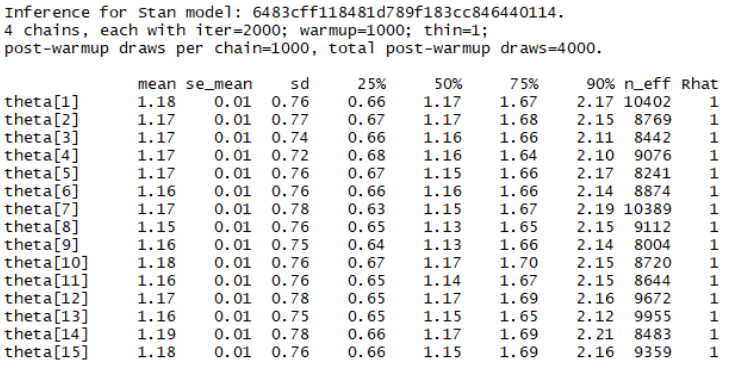
\includegraphics[scale=0.75]{tabela_15_normal01.png}
    \caption{Parte da tabela-resumo das estatísticas das estimativas dos $\theta's$ usando distribuições a \textit{priori} Normal padrão; a tabela mais completa pode ser encontrada nas figuras \ref{fig:tabelacompleta01}, \ref{fig:tabelacompleta02} e \ref{fig:tabelacompleta03}.}
    \label{fig:tabela01}
 \end{figure}
 
 \begin{figure}[!htbp]
    \centering
    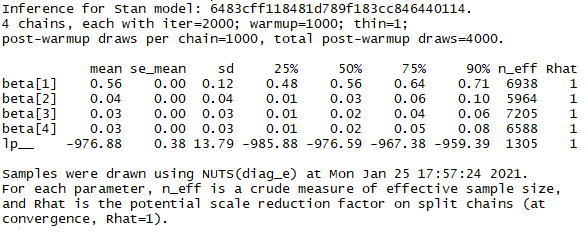
\includegraphics[scale=0.75]{tabela_todos_normal01_pt3_betas.png}
    \caption{Tabela-resumo das estatísticas das estimativas de $b$ usando distribuições a \textit{priori} Normal padrão.}
    \label{fig:tabela01beta}
 \end{figure}
 
 Conforme podemos conferir na tabela representada pelas figuras \ref{fig:tabelacompleta01}, \ref{fig:tabelacompleta02} e \ref{fig:tabelacompleta03}, as estimativas dos parâmetros $\theta$ convergiram. Uma amostra dessa tabela está na figura \ref{fig:tabela01}. A convergência das estimativas dos parâmetros $b$ pode ser verificada na tabela \ref{fig:tabela01beta}. 
 
 Uma vez que estamos confortáveis com a confiabilidade dos resultados, podemos verificar qual o comportamento dos mesmos. É interessante notar aqui que o tamanho da nossa amostra efetiva, n$\_$eff, é maior que o tamanho das observações, em todos os casos. Ao investigarmos essa questão, descobrimos que isso é justificável\footnote{Através da documentação do Stan, por sua vez a linguagem de nosso modelo. O manual está disponível em \url{https://mc-stan.org/docs/2_25/reference-manual/effective-sample-size-section.html}. Essa questão foi discutida e reforçada pelos seus desenvolvedores da linguagem em seu fórum oficial. Disponível em \url{https://discourse.mc-stan.org/t/n-eff-greater-than-number-of-iterations/7114} e \url{https://discourse.mc-stan.org/t/n-eff-bda3-vs-stan/2608}. Último acesso em 27/02/2021. \label{notastan}}, principalmente por conta do uso da amostragem do tipo No-U-turn sampling (NUTS), implementada no algoritmo usado no Stan, que produz esse efeito. Mais informações podem ser encontradas sobre esse assunto na documentação indicada na nota de rodapé \ref{notastan}.
 
 Olhando primeiramente para os parâmetros $b$ de dificuldade dos itens na figura \ref{fig:betas01}, uma informação é bastante chamativa: enquanto os itens 2, 3 e 4, que se referem às condições específicas de liberação legal do aborto, têm dificuldades com mediana e até mesmo terceiro quartil menores que 0.25, o item 1, que se refere à possibilidade genérica de aborto legal sob a vontade da mulher, tem mediana acima de 0.5 e terceiro quartil acima de 0.75. Isso mostra que a dificuldade $b$ em ser favorável ao item 1 é bem maior que a dificuldade $b$ dos itens 2, 3 e 4. Esse resultado é bastante alinhado às expectativas em relação ao tema --- em geral, é mais fácil ser favorável ao aborto em uma situação específica que em todas as situações possíveis.
 
 \begin{figure}[!htbp]
    \centering
    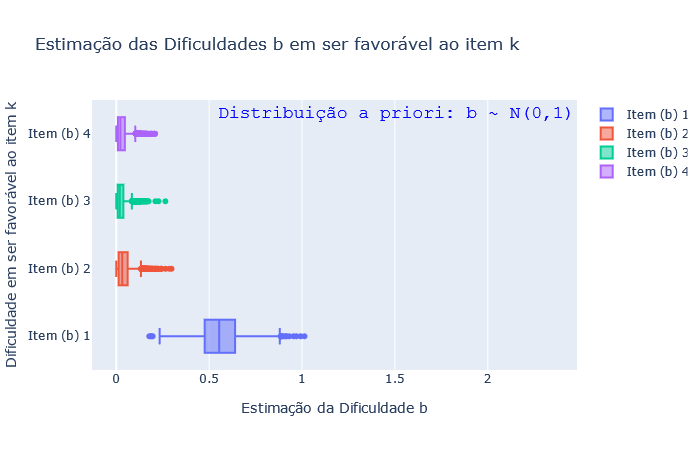
\includegraphics[scale=0.5]{betas_todos_normal01_py.png}
    \caption{\textit{Boxplots} das estimativas de dificuldades dos itens que representam condições específicas de permissão legal do aborto, usando distribuições a \textit{priori} Normal padrão.}
    \label{fig:betas01}
 \end{figure}
  \newpage
 Voltando-nos agora para as permissividades $\theta$ dos entrevistados, em especial para o histograma da mediana das estimativas representado na figura \ref{fig:thetas01}, podemos ver que nossas expectativas também tinham fundamento: os entrevistados estão mais concentrados em valores positivos de permissividade, sendo que mais da metade deles tem $\theta > 0.5$. Isso mostra uma sociedade progressista em relação ao assunto do aborto, conforme esperávamos.
 
 \begin{figure}[!htbp]
    \centering
    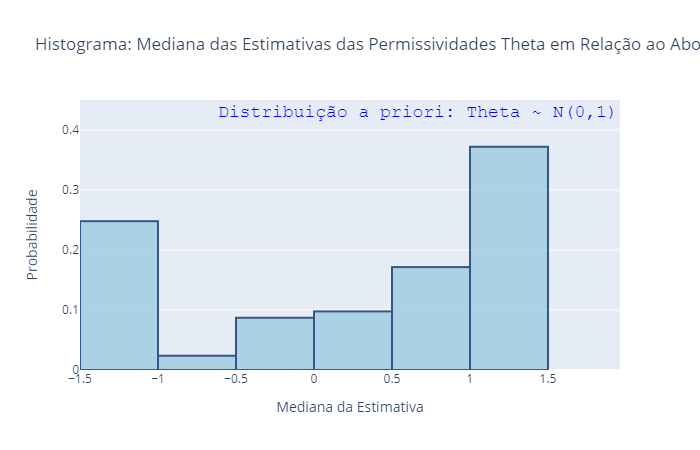
\includegraphics[scale=0.55]{histograma_thetas_mediana_todos_N01_py.png}
    \caption{Histograma das estimativas das permissividades $\theta$ dos entrevistados em relação ao aborto, usando distribuições \textit{a priori} Normal padrão.}
    \label{fig:thetas01}
 \end{figure}
 
 Outras visualizações de resultados geradas por essa análise estão disponíveis em \ref{extrapadrao}.
 
 \subsubsection*{Inferência dos parâmetros usando distribuições \emph{a priori} escolhidas}
 Vamos agora analisar as estimativas que obtivemos usando nossas impressões anteriores à visualização dos dados sobre a dificuldade dos itens e a permissividade dos entrevistados. Escolhemos uma distribuição \textit{a priori} para os itens $b \sim N(-0.2, 0.8)$ e $\theta \sim N(0.2, 0.8)$ para as permissividades.

 Podemos verificar que a convergência das estimativas dos parâmetros $\theta$ e $b$ é satisfatória.
 
 \begin{figure}[!htbp]
    \centering
    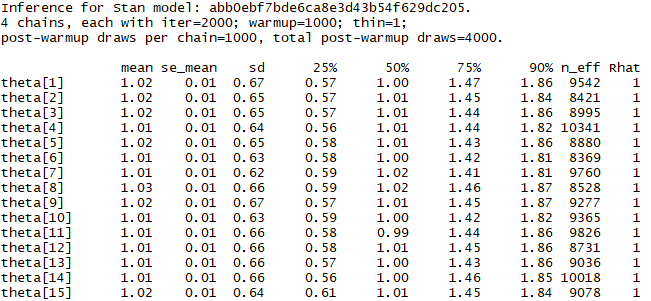
\includegraphics[scale=0.75]{tabela_0208_amostra.png}
    \caption{Parte da tabela-resumo das estatísticas das estimativas dos $\theta's$ usando distribuições \textit{a priori} $N(0.2, 0.8)$; a tabela mais completa pode ser encontrada nas figuras \ref{fig:tabelacompleta0208} e \ref{fig:tabelacompleta02082}.}
    \label{fig:tabela0208}
 \end{figure}
 
 \begin{figure}[!htbp]
    \centering
    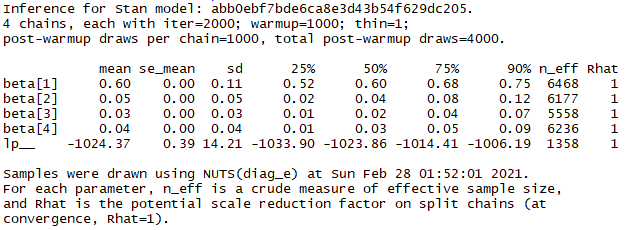
\includegraphics[scale=0.75]{tabela_0208_pt3_betas.png}
    \caption{Tabela-resumo das estatísticas das estimativas de $b$ usando distribuições \textit{a priori} $N(0.2, 0.8)$.}
    \label{fig:tabela0208beta}
 \end{figure}
 
 Uma vez verificada a validade das estimativas, analisaremos os resultados.
 
 Observando o \textit{boxplot} das distribuições das dificuldades $b$, podemos perceber que a mediana da dificuldade do item 1 é bastante maior que aquela dos itens 2, 3 e 4, assim como aconteceu utilizando as distribuições \textit{a priori} Normal padrão. Os resultados são bastante semelhantes e nos apontam para a dificuldade maior em ser favorável ao aborto sob vontade da mulher em relação a ser favorável ao aborto em casos específicos.
 
 \begin{figure}[!htbp]
    \centering
    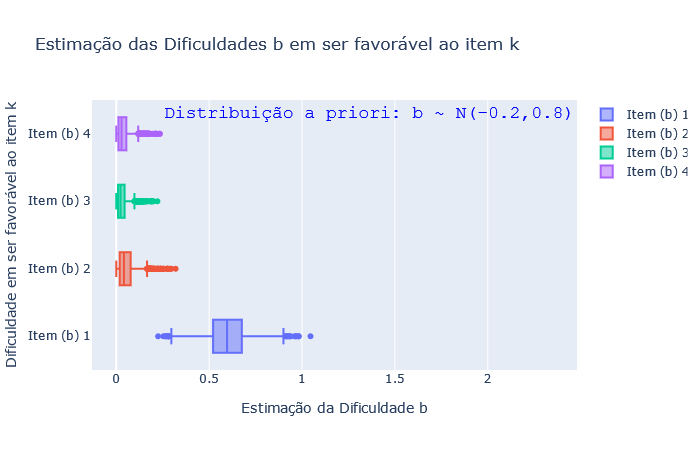
\includegraphics[scale=0.65]{boxplot_betas_R_0208.png}
    \caption{\textit{Boxplots} das estimativas de dificuldades dos itens que representam condições específicas de permissão legal do aborto, usando distribuições \textit{a priori} $b \sim N(-0.2, 0.8)$ e $\theta \sim N(0.2, 0.8)$.}
    \label{fig:betas0208}
 \end{figure}
 
 Analisando o histograma das estimativas das permissividades $\theta$ dos entrevistados, vemos novamente a característica progressista dos entrevistados em relação ao tema: mais da metade deles tem permissividade acima de 0.5, assim como indicado usando as distribuições \textit{a priori} Normal padrão; desta vez, porém, aqueles com permissividade maior (de 1 a 1.5) apareceram em menor frequência, enquanto houve aumento da frequência da permissividade entre 0.5 e 1. Isso é esperado, uma vez que nossas distribuições \textit{a priori} têm desvio padrão menor que aquelas com distribuição Normal padrão.
 
 \begin{figure}[!htbp]
    \centering
    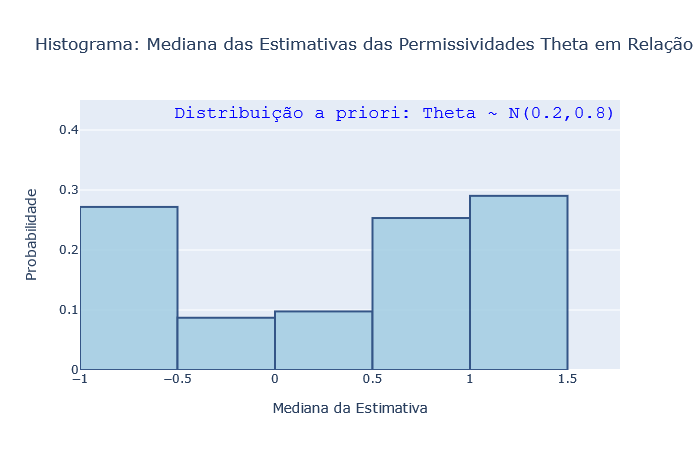
\includegraphics[scale=0.65]{hist_theta_mediana_0208.png}
    \caption{Histograma das estimativas das permissividades $\theta$ dos entrevistados em relação ao aborto, usando distribuições \textit{a priori} $b \sim N(-0.2, 0.8)$ e $\theta \sim N(0.2, 0.8)$.}
    \label{fig:thetas0208}
 \end{figure}
 
 Outras figuras geradas por essa análise estão em \ref{extraescolhida}.
 
 \newpage
 \subsubsection*{Inferência dos parâmetros usando distribuições \emph{a priori} pouco informativas}
 Para verificar o impacto da escolha das distribuições \textit{a priori} padrão e escolhidas por nós, estudamos também o mesmo modelo usando distribuições \textit{a priori} pouco informativas para $\theta$, $\theta \sim N(0, 100)$ e para $b$, $b \sim N(0, 100)$.
 
 Começaremos verificando a convergência das estimativas dos parâmetros.
 \begin{figure}[!htbp]
    \centering
    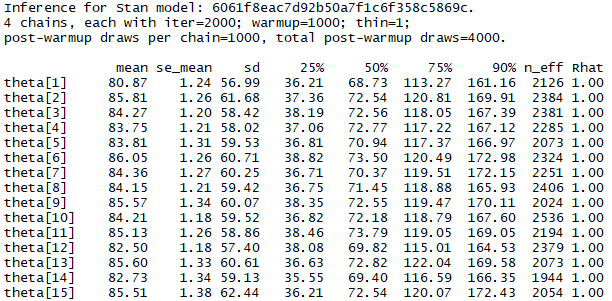
\includegraphics[scale=0.75]{tabela_0100_amostra.png}
    \caption{Parte da tabela-resumo das estatísticas das estimativas dos $\theta's$ usando distribuições \textit{a priori} $N(0, 100)$; a tabela mais completa pode ser encontrada nas figuras \ref{fig:tabelacompleta0100} e \ref{fig:tabelacompleta01002}.}
    \label{fig:tabela0100}
 \end{figure}
 
 \begin{figure}[!htbp]
    \centering
    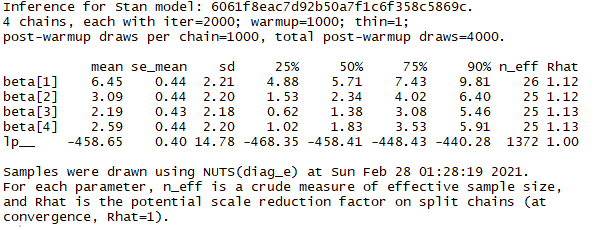
\includegraphics[scale=0.75]{tabela_0100_pt3_betas.png}
    \caption{Tabela-resumo das estatísticas das estimativas de $b$ usando distribuições \textit{a priori} $N(0, 100)$.}
    \label{fig:tabela0100beta}
 \end{figure}
 
 Podemos já verificar, de antemão, que nossas estimativas para os parâmetros $b$ não são satisfatórias. Com isso em mente, vamos verificar os resultados gerados.
 
 Em relação às estimativas de $b$, vemos que apesar da grande quantidade de \textit{outliers}, a configuração permanece semelhante. A mediana da dificuldade $b$ do item 1 é mais deslocada à direita comparada à mediana da dificuldade dos outros itens, como nos casos anteriores. Podemos observar, porém, que os valores absolutos estão em um conjunto maior em comparação com os anteriores. Enquanto o limite superior, incluindo \textit{outliers}, não passa muito de uma unidade nas estimativas anteriores, nesse caso temos \textit{outliers} que passam de 15 unidades.
 
 \begin{figure}[!htbp]
    \centering
    \includegraphics[scale=0.7]{betas_python_0100.png}
    \caption{\textit{Boxplots} das estimativas de dificuldades dos itens que representam condições específicas de permissão legal do aborto, usando distribuições \textit{a priori} $N(0, 100)$.}
    \label{fig:betas01}
 \end{figure}
 
 Em relação às estimativas de $\theta$, vemos que a maior parte dos entrevistados está depois do 0, sugerindo, novamente, uma característica progressista dessa amostra de entrevistados em relação ao aborto. Assim como aconteceu com a estimativa das dificuldades $b$, como a distribuição \textit{a priori} não ajudou a limitar o intervalo de estimativas, essa ficou mais dispersa. No caso do histograma das medianas das estimativas de $\theta$, essas variaram de -100 a 100, enquanto que nos casos anteriores tivemos uma variação máxima de -1.5 a 1.5.
 
 \begin{figure}[!htbp]
    \centering
    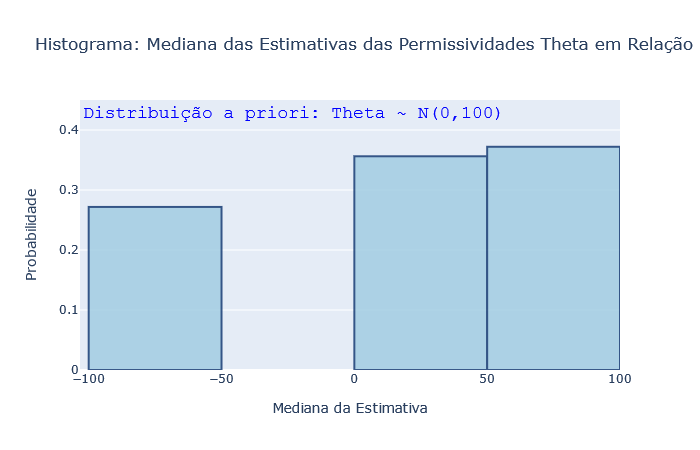
\includegraphics[scale=0.6]{hist_0100_theta_mediana.png}
    \caption{Histograma das estimativas das permissividades $\theta$ dos entrevistados em relação ao aborto, usando distribuições \textit{a priori} $N(0, 100)$.}
    \label{fig:thetas01}
 \end{figure}
 
 \begin{figure}[!htbp]
    \centering
    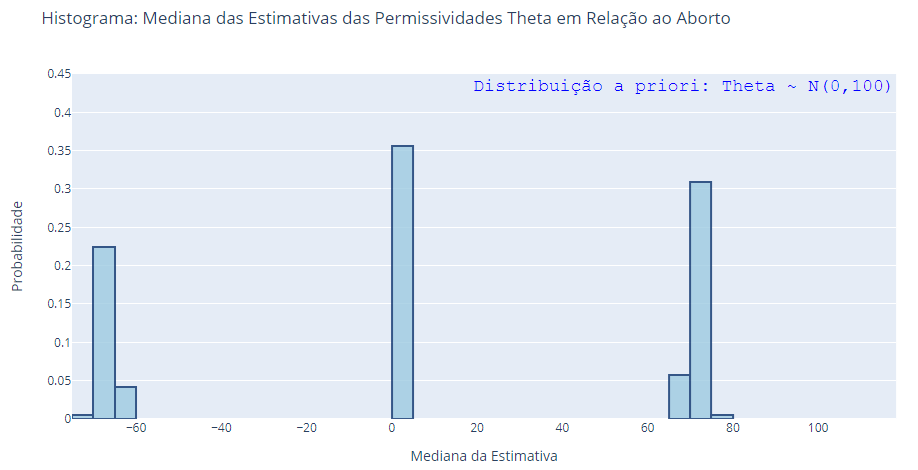
\includegraphics[scale=0.6]{hist_0100_alt.png}
    \caption{Histograma das estimativas das permissividades $\theta$ dos entrevistados em relação ao aborto, usando distribuições \textit{a priori} $N(0, 100)$, com 40 divisões.}
    \label{fig:thetas01b}
 \end{figure}
 
 Dessa maneira, podemos observar que, independente da escolha das distribuições \textit{a priori} serem mais ou menos informativas, as estimativas de dificuldade dos itens e a distribuição da mediana das permissividades têm interpretação semelhante. Ainda assim, há impacto notável no intervalo das estimações, ficando este mais disperso em caso da utilização de distribuições \textit{a priori} menos informativas. Mais figuras geradas por essa análise podem ser encontradas em \ref{extrapoucoinfo}.

% ---
% capitulo de Modelo
% ---

 \chapter{Modelo bayesiano de ponto ideal}\label{modelobarberasecao}
 Nosso objetivo é metrificar posicionamentos ideológico-feministas de cidadãos e figuras públicas presentes no Twitter, utilizando o modelo proposto por Barberá (\citeyear{barbera2015}). Originalmente, com esse mesmo modelo, o autor citado metrifica e compara diversas posições ideológicas político-partidárias de cidadãos e figuras públicas numa escala única.

 Eu seu artigo, Barberá (\citeyear{barbera2015}) define a ideologia que ele pretende metrificar como ``uma linha cujo fim à esquerda reflete uma posição extremamente liberal, e cujo fim à direita corresponde ao extremo conservadorismo''\footnote{Tradução nossa.} (\citeauthoronline{bafumi2005}, \citeyear{bafumi2005} apud \citeauthoronline{barbera2015}, \citeyear{barbera2015}, p. 4). Adaptando a definição à ideologia feminista, pensaremos essa última também como \emph{uma linha, cujo fim à esquerda reflete uma posição extremamente aderente aos ideais e reivindicações feministas, e cujo fim à direita reflete uma posição extremamente contrária aos mesmos}.

 Nossa hipótese chave para fazer esse exercício é a de que o modelo é flexível no que toca à dimensão latente calculada, que dependerá do conjunto de figuras públicas que estão sendo consideradas no cálculo (\citeauthoronline{barbera2015}, \citeyear{barbera2015}, p. 11). Sendo assim, todas as justificativas feitas pelo autor de como e porque o modelo funciona adequadamente serão mantidas.

 O modelo de Barberá é completamente baseado nas redes de seguidores de cada usuário, bem como dos seguidos pelo mesmo. Com essa estrutura, o autor argumenta que é possível aprimorar modelos anteriores que faziam aferições semelhantes (\citeauthoronline{barbera2015}, \citeyear{barbera2015}, p. 5). Barberá pretendia com o seu modelo não apenas classificar usuários, mas também \emph{medir e comparar continuamente o posicionamento político-partidário deles}; \emph{indicar a incerteza de suas estimativas} e \emph{colocar cidadãos comuns e legisladores numa escala comum passível de comparação}. As três características destacadas são os grandes diferenciais do seu modelo. Para mais detalhes sobre a literatura comportamental e estatística utilizada, ver Barberá (\citeyear{barbera2015}, pp. 4-7).
 
 \section{Apresentação do modelo}
 Dividimos os usuários do Twitter que vamos estudar em dois conjuntos. O primeiro, com tamanho $n$, é composto pelas contas de usuários comuns, que chamaremos de \emph{cidadãos} e representaremos por $i$, $i \in \{1, ..., n\}$. O segundo, de tamanho $m$, é formado pelas contas de pessoas públicas feministas e antifeministas, ou seja, legisladores e políticos profissionais, acadêmicos, comunicadores, jornalistas, e também partidos, coletivos e agremiações que \textit{twittam} sobre feminismo. Esse último grupo chamaremos de \emph{influenciadores} $j$, $j \in \{1, ..., m\}$. Cada cidadão $i$ tem a escolha de seguir ou não um influenciador $j$.

 Barberá fez essa divisão em grupos por motivos computacionais e também para ter um grupo de referência sobre o assunto estudado. Se cidadãos e influenciadores fossem analisados igualmente, sem o grupo pequeno de referência (o de influenciadores), a estimação ficaria computacionalmente intratável e ineficiente, uma vez que precisaríamos verificar todas as combinações possíveis de seguimento entre todos os usuários estudados, dois a dois. Além disso, sem o grupo de referência cuja característica marcante é justamente a variável latente de interesse, nosso estudo seria menos qualificado para estimar a mesma, uma vez que a decisão de seguir ou não um indivíduo não dependeria tanto dessa característica.
 
%  \section*{Parâmetros}
 Seja $y$ a variável que representa a decisão de um usuário seguir outro no Twitter. Se um cidadão $i$ decidir seguir um influenciador $j$, $y_{ij} = 1$; caso contrário, $y_{ij} = 0$. Barberá considera a variável latente \emph{ideologia} como unidimensional --- uma reta, conforme comentamos anteriormente. Ele espera então que a probabilidade de decisão de seguimento $P(Y=1)$ esteja em função da distância euclidiana entre a ideologia do cidadão $i$ e do influenciador $j$. Isso significa que a decisão de seguimento dependerá do quão distante o \emph{ponto ideal ideológico $\theta_{i}$ do cidadão $i$} estará do \emph{ponto ideal ideológico $\phi_{j}$ do influenciador $j$}.
 
 O autor propõe também a adição de dois parâmetros extra, relevantes para a metrificação: a \emph{popularidade $\alpha_{j}$ do influenciador $j$} e o \emph{interesse $\beta{i}$} (pelo assunto estudado --- no caso de Barberá, política partidária, e no nosso caso, feminismo) \emph{do cidadão $i$}. A consideração da popularidade $\alpha_{j}$ do influenciador $j$ se dá porque alguns influenciadores são mais prováveis de serem seguidos que outros, independente do ponto ideal da variável latente que estejamos querendo calcular. Uma influenciadora feminista de prestígio nacional, seja por ser uma grande acadêmica, como Débora Diniz, seja por ser uma artista muito popular, como MC Carol, ou por ter boas habilidades de comunicadora, como Sabrina Fernandes, tem mais chances de ser seguida que uma militante de um pequeno coletivo, que não tem tanta exposição em outras mídias, ou que não faz um uso tão profissional da plataforma. O interesse $\beta_{i}$ do cidadão $i$ no assunto de interesse também interfere na decisão do mesmo de seguir um influenciador $j$, e está correlacionado à quantidade de influenciadores do assunto estudado que esse cidadão segue. Cidadãos que têm mais interesse que a média da população pelas pautas feministas devem seguir mais contas de influenciadores feministas (ou antifeministas, dependendo do porquê do interesse), e, da mesma maneira, terão probabilidades maiores de seguir mais um influenciador que trate do assunto. Como essas informações são independentes da variável latente e influenciam na decisão de seguimento, ambas precisam ser consideradas.
 
 Feitas as considerações, a probabilidade de que um usuário $i$ siga um influenciador $j$ pode ser colocada como a seguinte formulação de um modelo logit (\citeauthoronline{barbera2015}, \citeyear{barbera2015}, p. 8):
 \begin{equation}
     P(y_{ij} = 1| \alpha_{j}, \beta_{i}, \gamma, \theta_{i}, \phi_{j}) = logit^{-1}(\alpha_{j} + \beta_{i} - \gamma ||\theta_{i} - \phi_{j}||^{2}).\label{probseguimento}
 \end{equation}
 Podemos ler essa formulação como a \emph{probabilidade do cidadão $i$ tomar a decisão de seguir o influenciador $j$ ($y_{ij} = 1$), dados os parâmetros $\alpha_{j}$ popularidade de $j$, $\beta_{i}$ interesse sobre o assunto estudado de $i$, $\theta_{i}$ ponto ideal ideológico de $i$, $\phi_{j}$ ponto ideal ideológico de $j$ e $\gamma$ constante de normalização da distância entre os pontos ideais, será o inverso do logit de $\alpha_{j} + \beta_{i} - \gamma ||\theta_{i} - \phi_{j}||^{2}$}. 
 
%  \section{Função de Verossimilhança}
 Nosso maior desafio estatístico é fazer a inferência dos conjuntos de parâmetros, $\theta = (\theta_{i}, ..., \theta_{n})', \phi = (\phi_{j}, ..., \phi_{m})', \alpha = (\alpha_{j}, ..., \alpha_{m})', \beta = (\beta_{i}, ..., \beta_{n})'$ e $\gamma$, uma vez que são todos variáveis latentes. Assumindo independência local de $y$ --- ou seja, assumindo que as decisões individuais de seguir são independentes entre os $n$ cidadãos e $m$ influenciadores, condicionadas aos parâmetros --- a função de verossimilhança pode ser escrita como
  \begin{equation}
     p(y| \alpha, \beta, \gamma, \theta, \phi) = \prod_{i=1}^{n} \prod_{j=1}^{m} (logit^{-1}(\pi_{ij}))^{y_{ij}} (1 - logit^{-1}(\pi_{ij}))^{1 - y_{ij}},\label{verossimilhancabarbera}
 \end{equation}
 onde $\pi_{ij} = \alpha_{j} + \beta_{i} - \gamma ||\theta_{i} - \phi_{j}||^{2}$ (\citeauthoronline{barbera2015}, \citeyear{barbera2015}, p. 8).
 
 Barberá (\citeyear{barbera2015}) considera distribuições a priori normais com um estrutura hierárquica.
 Assim, cada um dos quatro conjuntos de parâmetros ($\alpha, \beta, \theta, \phi$) tem distribuições tais que $\alpha_{j} \sim N(\mu_{\alpha}, \sigma_{\alpha})$, $\beta_{i} \sim N(\mu_{\beta}, \sigma_{\beta})$, $\theta_{i} \sim N(\mu_{\theta}, \sigma_{\theta})$ e $\phi_{j} \sim N(\mu_{\phi}, \sigma_{\phi})$ (\citeauthoronline{barbera2015}, \citeyear{barbera2015}, p. 8). É importante lembrar aqui que os parâmetros são independentes para todos os cidadãos e influenciadores. Dada essa definição, para todos os novos parâmetros gerados --- $\mu$ e $\sigma$ --- são designadas distribuições pouco informativas (ou \textit{``flat''}), com exceção de três casos: as médias $\mu_{\theta}$ e $\mu_{\alpha}$, que são fixadas em 0, e o desvio padrão $\sigma_{\theta}$, que é fixado em 1. Barberá justifica fixar os três valores por motivos de \textit{identificabilidade} (\citeauthoronline{barbera2015}, \citeyear{barbera2015}, p. 9).
 
 A partir da equação \ref{probseguimento},
 \begin{equation*}
     P(y_{ij} = 1| \alpha_{j}, \beta_{i}, \gamma, \theta_{i}, \phi_{j}) = logit^{-1}(\alpha_{j} + \beta_{i} - \gamma ||\theta_{i} - \phi_{j}||^{2}),
 \end{equation*}
 podemos notar que o modelo proposto não é identificável. Note que, por exemplo, ao adicionarmos uma constante qualquer $K$ aos parâmetros $\theta_{1}$ e $\phi_{1}$, temos $\theta^{*}$ = $\theta_{1} + K$ e $\phi^{*}=\phi_{1} + K$. Este novo conjunto de parâmetros irá implicar na mesma probabilidade, e consequentemente a função de verossimilhança nesses dois conjuntos de parâmetros será a mesma. Esse problema é conhecido como não identificabilidade e tem consequências na estimação dos parâmetros. Por exemplo, não há unicidade na estimativa de máxima verossimilhança.
 
 Esse tipo de problema é comum em modelos TRI, e algumas estratégias diferentes são empregadas para corrigi-lo. Nos materiais suplementares do artigo, em especial na página 12, Barberá justifica a escolha da distribuição $\theta_{i} \sim N(0, 1)$ afirmando que, além de conseguir identificação local com essa configuração, ela também facilita a interpretação dos resultados. Para atingir a identificação completa, ele define ainda valores iniciais para os influenciadores --- -1 para liberais e +1 para republicanos. De maneira semelhante, escolheremos -1 para feministas e +1 para antifeministas.

 A distribuição \emph{a posteriori} do modelo pode ser representada da seguinte maneira, considerando a função de verossimilhança \ref{verossimilhancabarbera} e as distribuições \emph{a priori} apresentadas em anteriormente:
 \begin{equation}
    \begin{aligned}
         p(\alpha, \beta, \gamma, \theta, \phi | y) &\propto p(\alpha, \beta, \gamma, \theta, \phi, \mu, \sigma)\\
         &\prod_{i=1}^{n} \prod_{j=1}^{m} logit^{-1}(\pi_{ij})^{y_{ij}} (1 - logit^{-1}(\pi_{ij}))^{1 - y_{ij}}\\
         &\prod_{j=1}^{m} N(\alpha_{j}|\mu_{\alpha}, \sigma_{\alpha}) \prod_{i=1}^{n} N(\beta_{i}|\mu_{\beta}, \sigma_{\beta}) \prod_{i=1}^{n} N(\theta_{i}|\mu_{\theta}, \sigma_{\theta}) \prod_{j=1}^{m} N(\phi_{j}|\mu_{\phi}, \sigma_{\phi})
     \end{aligned}
 \end{equation}
 conforme Barberá (\citeyear{barbera2015}, p. 9).
 
 \section{Estimação e inferência}
  Para fazer a estimação, devido à quantidade de parâmetros desse modelo, métodos de máxima verossimilhança ou mesmo numéricos encontram dificuldades, conforme já discutimos em \ref{posterioriintratavel}. Usamos então o método de simulação MCMC (ver Anexo \ref{mcmc}) para obter amostras da densidade \textit{a posteriori} de cada parâmetro do modelo.
 
 Visando aumentar a velocidade da estimação, Barberá divide a estimação em duas fases. Na primeira, o autor utiliza uma variação do algoritmo de amostragem hamiltoniana de Monte Carlo (HMC), chamada de No-U-Turn (NUTS), embutida no código da biblioteca RStan. Com esse aparato, ele estima os parâmetros associados aos influenciadores, indexados por $j$, através de uma amostra aleatória de dez mil cidadãos que seguem pelo menos 10 influenciadores. Na segunda etapa, é implementado no R o algoritmo de Metropolis-Hastings para estimar os parâmetros associados aos cidadãos, indexados por $i$. Cada um desses parâmetros pode ser estimado individualmente, uma vez que assumimos independência local dos mesmos, condicional aos parâmetros dos influenciadores. Isso permite que vários núcleos de processamento possam ser usados para rodar várias amostragens simultaneamente, aumentando bastante a velocidade computacional (\citeauthoronline{barbera2015}, \citeyear{barbera2015}, p. 10). Implementamos ambas as fases de maneira idêntica à proposta no artigo original.

 Em ambos os estágios, os amostradores são executados usando duas cadeias de Markov.

 Na primeira fase, iniciamos cada cadeia da seguinte maneira:
 \begin{itemize}
 \item para o ponto ideal do cidadão $\theta_{i}$ e a constante de normalização $\gamma$, com o sorteio aleatório de uma distribuição normal padrão multivariada;
 \item para as popularidades $\alpha_{j}$ dos influenciadores, com o logaritmo do número de seguidores do influenciador $j$ em questão;
 \item para interesse no assunto estudado $\beta_{i}$, com o logaritmo do número de influenciadores $j$ seguidos pelo cidadão $i$;
 \item e, para o ponto ideal do influenciador $j$ $\phi_{j}$, com valores -1 para influenciadores feministas e +1 para influenciadores antifeministas.
 \end{itemize}
 Esse início ``qualificado'' é feito visando aumentar a velocidade de convergência. Essa estratégia de ajuste de modelo se mostrou bastante robusta, segundo Barberá; os resultados finais encontrados por ele foram largamente insensíveis aos valores iniciais (\citeauthoronline{barbera2015}, \citeyear{barbera2015}, p. 10).
 
 Na segunda fase, uma vez que já temos todos os pontos ideais $\phi$ e as popularidades $\alpha$ dos influenciadores e a constante $\gamma$, nos resta apenas encontrar os pontos ideais $\theta$ e os interesses $\beta$ dos cidadãos. Usamos então o algoritmo de Metropolis-Hastings para estimar os parâmetros faltantes, utilizando os demais parâmetros já encontrados. Para isso, é considerado o logaritmo do número de influenciadores $j$ seguidos pelo cidadão $i$ para inicializar o parâmetro interesse no assunto estudado $\beta_{i}$, e o sorteio aleatório de uma distribuição normal padrão para o ponto ideal do cidadão $\theta_{i}$.
 
 \section{Amostra}
 Para obter nossa amostra qualificada de feministas e antifeministas, começamos identificando um conjunto de influenciadores que tocavam recorrentemente no assunto feminismo, seja pelo seu apoio ou pela sua negação\footnote{Uma minibiografia somada a uma pequena justificativa do porquê da escolha de cada influenciador pode ser encontrada no Anexo \ref{justificativa}.}. Escolhemos diversas contas do Twitter, todas públicas, com os seguintes perfis distintos: 
 \begin{itemize}
 \item representantes políticos (em exercício ou não) que tenham posicionamento público sobre feminismo;
 \item acadêmicos, pesquisadores e estudiosos do feminismo, ou de assuntos similares/tangentes;
 \item comunicadores --- jornalistas, escritores, blogueiros, \emph{podcasters}, artistas --- que twittam sobre feminismo;
 \item coletivos favoráveis ou contrários ao feminismo; 
 \item institutos de pesquisa com posicionamento público sobre feminismo;
 \item meios de comunicação --- jornais, revistas, grandes \textit{blogs}, \emph{podcasts} --- que tratem do assunto feminismo. 
 \end{itemize}
 Dividimos essas contas em favoráveis ou contrárias ao feminismo de acordo com suas convicções públicas, seja de acordo com as bandeiras feministas ou contrárias a ela, de acordo com as características que levantamos no capítulo de introdução (ver \ref{caractfem} e \ref{caractantifem}). Seguindo esse método, escolhemos um total de $m$ = 266 influenciadores.

 Usamos então a API do Twitter e obtivemos a lista de todos os $n$ cidadãos seguidores dos $m$ influenciadores previamente escolhidos. De saída, estimamos ter mais de 6 milhões de cidadãos para analisar. A obtenção desses dados foi longa e custosa, porém, demorando por volta de 20 dias para ser completamente concluída. Com todos os percalços do caminho, obtivemos informações de um total de $n$ = 4.770.287 cidadãos ao final dessa primeira extração. 

 Da mesma maneira que Barberá (\citeyear{barbera2015}, p. 12), observamos que uma grande parte dessas contas eram inativas, ou \textit{spam/bots}, ou residiam fora do Brasil. Assim, inspirados nos filtros propostos pelo autor, excluímos os usuários que:
 \begin{itemize}
 \item enviaram menos de 50 tweets;
 \item não mandaram nenhum tweet em 2020, ano de extração dos dados;
 \item tinham menos de 20 seguidores;
 \item residiam fora do Brasil ou não tinham informações de localidade disponíveis;
 \item seguiam menos de 3 influenciadores considerados. 
 \end{itemize}
 A nossa amostra final, seguindo esses parâmetros mínimos, foi de $n$ = 382.934 cidadãos.

 \subsection{Considerações sobre nossa amostra de dados}
 Os usuários do Twitter não são uma amostra representativa da população do país de origem dos mesmos. Eles têm características populacionais próprias, diferentes. Os usuários do Twitter dos Estados Unidos, por exemplo, têm média de idade menor que a da população do país, e maiores rendimentos anuais que a mesma (\citeauthoronline{barbera2015}, \citeyear{barbera2015}, p. 12). Não temos as mesmas informações comparativas entre os usuários do Twitter do Brasil e a população brasileira, mas pensamos que essas populações também, provavelmente, terão diferenças demográficas significativas entre si. Questões desde acesso à internet até nível de conhecimento tecnológico necessário para acessar o Twitter, ou mesmo tempo livre para fazê-lo, devem distanciar o usuário brasileiro médio do Twitter do cidadão brasileiro médio genérico. Não podemos dizer, então, que a população brasileira usuária do Twitter é uma boa amostra para representar a população brasileira em geral.

 Além disso, nossa amostra é igualmente não representativa de todo o conjunto de usuários seguidores dos influenciadores selecionados, uma vez que foi escolhido manter apenas aqueles que seguiam uma série de pré-requisitos. Apesar de excluir a maior parte dos cidadãos pré-selecionados, a aplicação dos filtros é positiva para a precisão da inferência dos pontos ideais dos influenciadores, uma vez que as contas filtradas podem ser consideradas mais confiáveis, dado seu comportamento no Twitter e sua quantidade de seguidores, e com mais ``autoridade'' em relação ao assunto estudado, pois seguem pelo menos 3 influenciadores do tema escolhido. Sendo assim, analisar o comportamento de seguimento dos cidadãos contidos na amostra final pode ser altamente informativo sobre posicionamentos ideológicos dos influenciadores, mesmo que essa amostra não seja representativa nem do país, nem do conjunto de influenciados em geral sobre o tema (\citeauthoronline{barbera2015}, \citeyear{barbera2015}, p. 12).

 Barberá afirma que todo o procedimento de estudo de comportamento de seguimentos desses cidadãos selecionados é em algum grau análogo a uma pesquisa (ou \emph{survey}) com muitos entrevistados, onde cada entrevistado provê uma quantidade pequena de informação que, quando agregada, resulta em estimações políticas altamente acuradas (\citeauthoronline{barbera2015}, \citeyear{barbera2015}, p. 12).
 
 % ---
 % capitulo dos Resultados
 % ---
 
 \chapter{Análise dos resultados}
 Uma vez gerados os resultados das duas fases de inferência, obtemos uma série de estatísticas para todos os nossos parâmetros de interesse. Na primeira fase, obtemos o ponto ideal $\phi$ e a popularidade $\alpha$ dos influenciadores e a constante de normalização $\gamma$ do modelo, enquanto na segunda fase obtemos o ponto ideal $\theta$ e o interesse no assunto estudado $\beta$ dos cidadãos. Exploramos os resultados encontrados nas sessões a seguir.
 
 \section{Resultados da primeira fase: influenciadores}
 Na primeira fase estimamos o ponto ideal $\phi$ e a popularidade $\alpha$ dos influenciadores dentro de um grupo dez mil cidadãos que seguem mais de 10 dos influenciadores escolhidos, e fazemos um filtro que seleciona apenas os influenciadores que são seguidos por mais de duzentos desses cidadãos selecionados. Por consequência, reduzimos a quantidade de influenciadores de que obtivemos estimações. Outros resultados interessantes encontrados nessa fase são o ponto ideal $\theta$ e o interesse no assunto estudado $\beta$ dos dez mil cidadãos. Eles não são um conjunto representativo de toda a amostra, uma vez que não foram sorteados aleatoriamente. Ainda assim seus resultados podem ser interessantes, pois se referem provavelmente aos cidadãos mais interessados que temos\footnote{Partindo-se do pressuposto de que há correlação entre a quantidade de influenciadores de terminado assunto que o cidadão segue com o interesse que ele tem pelo tema.}.
 
 Vamos começar a análise verificando a qualidade dos resultados encontrados para $\phi$, $\alpha$, $\theta$ e $\beta$.
 
 Começando pelo ponto ideal $\phi$ dos influenciadores, podemos observar na figura \ref{convphi} que houve convergência na amostra exibida pela tabela. De fato, ao analisarmos com mais cuidado os $\phi's$ gerados, todos os R-chapéus\footnote{O R-chapéu mede a convergência de uma Cadeia de Markov. Falamos um pouco mais sobre essa estimativa em \ref{normalpadraoinf}.} são no máximo 1. Uma tabela com mais dados pode ser obtida na parte de anexos, mais precisamente na figura \ref{convphianexo}.

 \begin{figure}[!htbp]
    \centering
    \includegraphics[scale=0.8]{tabela_phi_ponto_ideal_politico_incompleta_fase1_c_15.png}
    \caption{Amostra das estatísticas geradas para as estimações feitas para as distribuições \textit{a posteriori} dos parâmetros $\phi$.}
    \label{convphi}
 \end{figure}
 
 Olhando para as popularidades $\alpha$ na figura \ref{convalpha}, vemos que não obtivemos resultados tão satisfatórios quanto para os pontos ideais $\phi$. Além de um baixo número efetivo da amostra analisada, o R-chapéu das estimativas está alto, superando 1.1 em todas as linhas observadas. Uma tabela mais completa dessas estatísticas de $\alpha$ está disponível na figura \ref{convalphaanexo}.
 
 \begin{figure}[!htbp]
    \centering
    \includegraphics[scale=0.8]{tabela_alpha_popularidade_politico_incompleta_fase1_nc_15.png}
    \caption{Amostra das estatísticas geradas para as estimações feitas para as distribuições \textit{a posteriori} dos parâmetros $\alpha$.}
    \label{convalpha}
 \end{figure}
 \newpage
 Analisando então os pontos ideais $\theta's$ dos cidadãos na figura \ref{convtheta}, observamos bons valores de R-chapéu e de amostra efetiva analisada, sugerindo estimativas confiáveis para esses parâmetros. Mais informações das estimativas encontradas para os $\theta's$ estão disponíveis na figura \ref{convthetaanexo}.

 \begin{figure}[!htbp]
    \centering
    \includegraphics[scale=0.8]{tabela_theta_ponto_ideal_cidadao_incompleta_fase1_c_15.png}
    \caption{Amostra das estatísticas geradas para as estimações feitas para as distribuições \textit{a posteriori} dos parâmetros $\theta$.}
    \label{convtheta}
 \end{figure}
 
 Finalmente, observando a figura \ref{convbeta}, nos parece que houve boa estimação para os parâmetros de interesse $\beta$ dos cidadãos: nenhum dos $\beta's$ da figura supera o R-chapéu de 1.1. Uma visão mais completa desses parâmetros está na figura \ref{convbetaanexo}.

 \begin{figure}[!htbp]
    \centering
    \includegraphics[scale=0.8]{tabela_beta_interesse_cidadao_incompleta_fase1_c_15.png}
    \caption{Amostra das estatísticas geradas para as estimações feitas para as distribuições \textit{a posteriori} dos parâmetros $\beta$.}
    \label{convbeta}
 \end{figure}
 
 Conferindo os valores via código, de fato observamos ter estimações aparentemente confiáveis para $\phi$, $\theta$ e $\beta$, e estimações não confiáveis para $\alpha$. No entanto, essa fraqueza não impacta muito nosso estudo, pois nossos maiores interesses são os pontos ideais $\phi$ e $\theta$. Vamos nos concentrar nesses pontos, começando por $\phi$.
 
 \subsection*{Análise dos pontos ideais $\phi$ dos influenciadores}\label{ptoidealinf}
 Nosso primeiro interesse foi visualizar a distribuição dos influenciadores ao longo dos pontos ideais. Obtivemos então o histograma que se assemelha a uma distribuição bimodal que está representado na figura \ref{histresultados}. Na parte de cima do histograma vemos ainda um conjunto de linhas horizontais, que representa cada um dos influenciadores analisados.

 \begin{figure}[!htbp]
    \centering
    \includegraphics[scale=0.6]{hist_resultados.png}
    \caption{Histograma da média dos pontos ideais $\phi$ encontrados para os influenciadores.}
    \label{histresultados}
 \end{figure}
 
 Alguns pontos chamam atenção na distribuição. O primeiro é que existe uma separação evidente entre os dois lados, com pouquíssimos influenciadores perto do zero. Do lado esquerdo, em roxo, observamos a distribuição das influenciadores que classificamos, antes de ver os resultados de ponto ideal, como feministas. Esse grupo é composto apenas por mulheres, então sempre que nos referirmos a elas, o faremos no feminino. Podemos observar que não há nenhuma influenciadora entre 0 e -0.5, e apenas uma entre -0.5 e -1. Isso parece sugerir que o grupo feminista tem pouco meio-termo ideológico. Do outro lado, no agrupamento que classificamos de antemão como antifeminista, existe um grupo pequeno entre 0 e 1. Esse grupo, porém, parece estar de certa maneira separado do grupo com ponto ideológico maior que 0.5, uma vez que há alguma consistência de pessoas nesse começo, uma dispersão, e então outro grupo mais consistente de pessoas.
 
 Para aprofundar essa visualização, construímos um gráfico que compara a média das estimações de ponto ideal do influenciador com o número  de seguidores que ele tem relativamente ao influenciador com mais seguidores. Obtivemos, então, a figura \ref{pontoidealsegrel}. Fizemos a comparação, também, da média das estimações do ponto ideal do influenciador com o número de seguidores \textit{analisados pelo modelo} que ele tem relativamente ao influenciador que teve mais seguidores analisados. Essa segunda visualização está representada na figura \ref{pontoidealsegrelan}.

 \begin{figure}[!htbp]
    \centering
    \includegraphics[scale=0.8]{pontoideal_segrel.png}
    \caption{Comparação da média das estimações dos pontos ideais $\phi$ dos influenciadores com a quantidade de seguidores desse influenciador relativamente ao influenciador com mais seguidores.}
    \label{pontoidealsegrel}
 \end{figure}

 \begin{figure}[!htbp]
    \centering
    \includegraphics[scale=0.8]{pontoideal_segrelan.png}
    \caption{Comparação da média das estimações dos pontos ideais $\phi$ dos influenciadores com a quantidade de seguidores analisados pelo código desse influenciador relativamente ao influenciador com mais seguidores analisados pelo código. Esse gráfico está completo nos anexos, com todos os influenciadores identificados. Consulte a figura \ref{pontosideaistodos}.}
    \label{pontoidealsegrelan}
 \end{figure}
 
 O primeiro ponto que chama atenção comparando-se as figuras \ref{pontoidealsegrel} e \ref{pontoidealsegrelan} é que na primeira, em que apenas o número absoluto de seguidores importa, o ponto mais alto, representando o influenciador Jair Bolsonaro, está bastante isolado, enquanto na segunda, em que o número de seguidores analisados pelo código é o que conta, o isolamento do mesmo ponto é consideravelmente menor. Esse efeito sugere que o filtro de seguidores inativos ou falsos pode ter atingido de maneira desproporcional os seguidores desse influenciador em relação aos demais. Efeito semelhante aconteceu com a influenciadora Aline Barros, que era a que mais se aproximava de Bolsonaro na figura \ref{pontoidealsegrel}. Na figura \ref{pontoidealsegrelan}, Aline Barros não figura sequer entre as maiores dez contas analisadas.
 
 Outro ponto bastante interessante rapidamente percebido no gráfico é que pessoas com associações diretas geralmente estão próximas. Três exemplos podem ser colocados aqui: o primeiro, da família Bolsonaro, que estão bastante próximos ideologicamente, perto do ponto ideal +1; o segundo, das apresentadoras do \textit{podcast} Mamilos, que estão muito próximas, no ponto ideal -1.6; e o terceiro, dos músicos evangélicos, que representam a maior parte daqueles que têm ponto ideal entre 0 e 0.2.

 \begin{figure}[!htbp]
    \centering
    \includegraphics[scale=0.5]{bolsofamily.png}
    \caption{Localização da família Bolsonaro nos pontos ideais. De cima para baixo: Jair Bolsonaro, Eduardo Bolsonaro, Carlos Bolsonaro e Flavio Bolsonaro.}
    \label{bolsofamily}
 \end{figure}

 \begin{figure}[!htbp]
    \centering
    \includegraphics[scale=0.5]{mamileiras.png}
    \caption{Localização das \textit{podcasters} do programa Mamilos nos pontos ideais. As apresentadoras Ju Wallauer e Cris Bartis são tão próximas que praticamente se sobrepõem.}
    \label{mamileiras}
 \end{figure}

 \begin{figure}[!htbp]
    \centering
    \includegraphics[scale=0.55]{musicosevangelicos.png}
    \caption{Localização de cantores evangélicos nos pontos ideais. Esse grupo bastante coeso é formado por Aline Barros, Fernanda Brum, Ana Paula Valadão Bessa, Bruna Karla, André Valadão, David M. Quinlan, Marcelo Crivella (mais à direita) e Magno Malta (bem mais à direita). É interessante notar que os dois que se afastam mais do grupo, Crivella e Malta, são mais conhecidos por outros motivos: ambos são políticos. Esse fato deve influenciar na combinação das suas redes e portanto em seus pontos ideais calculados. Outro ponto importante é que apesar de se afastar, Crivella está mais próximo dos músicos religiosos que Malta. Isso talvez se deva à maior associação de Crivella com a igreja evangélica: o político é sobrinho de Edir Macedo, que está representado pelo ponto cinza mais próximo de 0, e que está exatamente ao lado de Crivella no gráfico.}
    \label{musicosevangelicos}
 \end{figure}
 
 Feitas essas observações, vamos nos aprofundar em cada \textit{cluster} representado nos gráficos. Investigaremos a linha ideológica da esquerda para a direita.
 
 Começando nossa análise pelo grupo das feministas, notamos algumas características ao longo da reta. Em primeiro lugar, é bastante perceptível que as influenciadoras que se declaram negras estão mais concentradas no extremo à esquerda, ficando cada vez mais raras ao longo da reta\footnote{É importante assinalarmos que pode ter acontecido de não estarmos considerando todas as negras autodeclaradas, pois é possível que não tenhamos encontrado declarações de negritude de alguma delas. Estão aqui identificadas todas as influenciadoras de quem encontramos autodeclaração publicamente disponível. Apesar dessa consideração, caso tenha acontecido de alguma influenciadora não ter sido identificada, será uma exceção.}. De maneira semelhante, as influenciadoras transgêneras (trans) também estão mais concentradas à esquerda da reta, ficando cada vez mais raras ao longo da mesma.

 \begin{figure}[!htbp]
    \centering
    \includegraphics[scale=0.55]{negrastrans.png}
    \caption{Influenciadoras Negras ou Trans feministas ao longo da reta ideológica. Note que estamos olhando apenas para o lado feminista do gráfico.}
    \label{negrastrans}
 \end{figure}
 
 Entre os pontos ideais estimados de -2.5 a -2, apenas duas influenciadoras não são autodeclaradas negras nem são trans: Louie Ponto e Débora Baldin. Ambas são ativistas lésbicas e já produziram juntas conteúdo para seus respectivos canais no Youtube.
 
 Avançando na reta dos pontos ideais estimados, a partir de -2 começamos a encontrar as mídias feministas. Novamente a questão de raça se faz presente. Da esquerda para a direita encontramos, em ordem, as mídias Blogueiras Negras e Geledés -- Instituto da Mulher Negra, ambas criadas por e para negras, seguidas por Não me Kahlo, Blogueiras Feministas, Tese Onze, Revista AzMina e ONU Mulheres Brasil, mídias sem o foco de raça. Veja as mídias feministas destacadas na reta de pontos ideais estimados do lado feminista na figura \ref{midiasfem}.

 \begin{figure}[!htbp]
    \centering
    \includegraphics[scale=0.55]{midasfem.png}
    \caption{Pontos ideais x tamanho relativo de seguidores analisados de mídias feministas. Note que estamos olhando apenas para o lado feminista do gráfico.}
    \label{midiasfem}
 \end{figure}
 
 Nos pontos ideais estimados de -1.8 a -1.6, encontramos os do Instituto Marielle Franco\footnote{O Instituto Marielle Franco é o único coletivo político feminista que não é compreendido também enquanto mídia feminista no escopo deste trabalho. Por conta disso, não faremos uma interpretação separada de coletivos políticos feministas da maneira que faremos para os coletivos políticos antifeministas ao final desta seção.} --- construído em memória de Marielle, vereadora feminista negra e lésbica assassinada no Rio de Janeiro --- e também as estimações de Anielle Franco, irmã de Marielle, e de Mônica Benício, viúva da vereadora. A partir desse intervalo também começamos a ver mais políticas e militantes filiadas a partidos. Entre os pontos ideais estimados -1.7 e -1.4 estão mais feministas filiadas ao Partido Socialismo e Liberdade (PSOL), aumentando a partir daí a quantidade de filiadas ao Partido Comunista do Brasil (PCdoB) e ao Partido dos Trabalhadores (PT). Veja a dispersão dos pontos ideais estimados de feministas, coloridos por partido, na figura \ref{partidasfem}.

 \begin{figure}[!htbp]
    \centering
    \includegraphics[scale=0.55]{partidasfem.png}
    \caption{Pontos ideais x tamanho relativo de seguidores analisados de filiadas feministas. Note que estamos olhando apenas para o lado feminista do gráfico.}
    \label{partidasfem}
 \end{figure}

 \begin{figure}[!htbp]
    \centering
    \includegraphics[scale=0.55]{partidosfem.png}
    \caption{Pontos ideais estimados para as configurações partidárias feministas.}
    \label{partidosfem}
 \end{figure}
 
 \newpage
  
 A partir dos pontos ideais estimados -1.4 até o final do grupo feminista, as influenciadoras analisadas não partidarizadas são, em geral, jornalistas. Encontramos nesse intervalo comunicadoras e jornalistas como Amanda Audi, Cynara Menezes e Mônica Bergamo. Outros dois pequenos agrupamentos que são interessantes destacar nesse intervalo são o da cineasta Petra Costa junto com a roteirista Antônia Pellegrino, feministas que foram responsáveis respectivamente pela direção e roteiro do documentário indicado ao Oscar ``Democracia em Vertigem'', e o agrupamento de Laura Carvalho, Rosana Pinheiro-Machado e Marcia Tiburi, três acadêmicas.
 
 Feita a análise do lado feminista, uma última característica nos chama atenção: influenciadoras mais isoladas, com menos ligações fortes com o grupo principal, parecem tender a ficar mais ao extremo.
 
 Vamos agora nos aprofundar no grupo antifeminista. Entre os pontos ideais estimados de 0 a 0.5, conforme já mostramos em \ref{musicosevangelicos}, estão principalmente concentrados os músicos evangélicos. Também estão presentes evangélicos não músicos, como Edir Macedo e Silas Malafaia, além do coletivo político Movimento Brasil Livre (MBL) e dois de seus maiores representantes: Kim Kataguiri e Fernando Holiday, que rompeu com o coletivo em janeiro de 2021, alguns meses depois dos dados deste trabalho terem sido coletados.
 
 Entre os pontos ideais estimados 0.5 e 0.7 observamos outros influenciadores que não compõem o conjunto de influenciadores antifeministas mais agrupado (com ponto ideal maior que 1), apesar de se aproximarem mais dele: o senador Carlos Viana, um político mais moderado em termos de feminismo (veja o Anexo \ref{justificativa}), a deputada Dayane Pimentel, a psicóloga cristã Marisa Lobo e as páginas do Partido Social Liberal (PSL) e da mídia Caneta Desesquerdizadora. Ao nosso ver, exceto pelo caso do senador, que é mais moderado, os demais influenciadores citados têm posições antifeministas bastante colocadas. Uma hipótese possível que justificaria a deputada e a psicóloga estarem fora do agrupamento maior antifeminista poderia ser a religiosidade cristã de ambas ser mais marcante que a do conjunto mais agrupado de antifeministas. Em relação ao PSL, uma hipótese possível é que o fato da conta pertencer a um partido, em especial um com tantos políticos eleitos quanto o PSL, pode ter efeito moderador sobre o ponto ideal calculado para ela. Talvez muitos cidadãos com possíveis pontos de vista diferentes podem seguir esse tipo de partido para se informar do que acontece politicamente, independentemente de concordarem com ele ou não. De maneira semelhante, essa hipótese pode ser válida para páginas como a da Caneta Desesquerdizadora, cujas publicações já fizeram muito sucesso na rede social: pessoas com pontos de vista distintos ao da página talvez a sigam para acompanhar quais conteúdos que pessoas com posicionamentos contrários aos delas consomem. Ficaremos com essas hipóteses como potenciais estudos para pesquisas futuras.
 
 Avançando para os pontos ideais estimados maiores que 0.7, a quantidade de influenciadores filiados a partidos aumenta consideravelmente. Diferentemente do lado feminista, que tem filiações a apenas quatro partidos diferentes, o lado antifeminista conta com quinze partidos distintos. É interessante comentar nesse sentido que, ao analisar os influenciadores partidarizados, notamos que vários mudaram muitas vezes de partido, fenômeno muito mais raro entre as influenciadoras feministas. Para efeitos de análise, deixamos registrado apenas o último partido do influenciador --- mesmo que esse tenha ficado sem partido depois, como no caso de Jair Bolsonaro, que está aqui analisado enquanto filiado ao PSL. 
 
 Teceremos comentários apenas sobre os três partidos com mais representantes no estudo: o Partido Social Liberal (PSL), com vinte e um influenciadores filiados, o Partido Republicanos, com oito influenciadores filiados, e o Partido Renovador Trabalhista Brasileiro (PRTB), com cinco influenciadores filiados. Influenciadores filiados ao PSL começam a estar presentes próximos do ponto ideal estimado 0.6, mas vão aumentando em volume ao longo da reta. A maior concentração dos filiados ao PSL está próxima ao ponto ideal estimado 1.5. Os filiados ao Partido Republicanos têm comportamento semelhante: começam em um ponto ideal estimado baixo, nesse caso por volta de 0.4, e aumentam ao longo da reta, se concentrando principalmente próximos do ponto ideal estimado 1.5. Por fim, os filiados ao PRTB têm um comportamento diferente. Começam a aparecer já próximos de 1.5, onde se concentram, mas vão mais longe na reta que os filiados aos partidos anteriores, alcançando o ponto ideal estimado de 1.8. O comportamento dos filiados a esses partidos está representado na figura \ref{partidosantifem}.
 
 \begin{figure}[!htbp]
    \centering
    \includegraphics[scale=0.6]{partidosantifem.png}
    \caption{Pontos ideais estimados para as configurações partidárias mais comuns entre os antifeministas.}
    \label{partidosantifem}
 \end{figure}
 
 \begin{figure}[!htbp]
    \centering
    \includegraphics[scale=0.8]{policosantifem_label.png}
    \caption{Pontos ideais estimados para antifeministas. Influenciadores políticos destacados. Note que estamos olhando apenas para o lado antifeminista do gráfico.}
    \label{politicosantifem}
 \end{figure}
 
 Entre os não políticos classificados em pontos ideais estimados entre 0.7 e 1.2 é interessante destacar os influenciadores Olavo de Carvalho, Alexandre Garcia e Ana Paula Henkel. Os três estão bastante próximos ao agrupamento da família Bolsonaro; Olavo de Carvalho está entre Flávio e Eduardo Bolsonaro, e Alexandre Garcia e Ana Paula Henkel um pouco deslocados à direita da família. Damares Alves e Carla Zambelli, respectivamente ministra do governo Bolsonaro e deputada apoiadora dele, também se encontram próximas ideologicamente à família Bolsonaro.
 
 A partir dos pontos ideais estimados em 1, podemos notar uma concentração maior de mídias e jornalistas antifeministas. Em relação às mídias, com pontos ideais estimados disponíveis na figura \ref{midiasantifem}, estão, em ordem, a página Caneta Desesquerdizadora, o portal Senso Incomum, o jornal Conexão Política, a produtora Brasil Paralelo, a página Família Direita Brasil, o jornal Crítica Nacional, o portal Terça Livre, e, finalmente, o jornal Brasil Sem Medo. Entre os jornalistas e comunicadores, com representação disponível na figura \ref{jornalistasantifem}, é interessante destacar, em relação aos pontos ideais estimados: entre 1.1 e 1.5, os comentaristas políticos Rodrigo Constantino e Ana Paula Henkel, além do colunista Leandro Ruschel, dos jornais Brasil Sem Medo e Conexão Política, cujo ponto ideal estimado é quase o mesmo que o desta última mídia; entre 1.5 e 1.7, a jornalista e assessora política Sarita Coelho, que aparece ao lado do seu assessorando Bruno Engler; e, finalmente, acima de 1.7, o \textit{youtuber} e presidente do Movimento Conservador, Edson Salomão, que aparece ao lado do político Douglas Garcia, vice-presidente do mesmo movimento, esse último classificado com o maior ponto ideal estimado do nosso estudo.

 \begin{figure}[!htbp]
    \centering
    \includegraphics[scale=0.6]{jornalistasantifem.png}
    \caption{Pontos ideais x tamanho relativo de seguidores analisados de jornalistas antifeministas. Note que estamos olhando apenas para o lado antifeminista do gráfico.}
    \label{jornalistasantifem}
 \end{figure}

 \begin{figure}[!htbp]
    \centering
    \includegraphics[scale=0.8]{midias_antifem_label.png}
    \caption{Pontos ideais x tamanho relativo de seguidores analisados de mídias antifeministas. Note que estamos olhando apenas para o lado antifeminista do gráfico.}
    \label{midiasantifem}
 \end{figure}
 
 Por fim, vamos comentar as estimações de ponto ideal para os coletivos políticos que consideramos antifeministas. Apesar desses coletivos estarem espalhados ao longo da reta ideológica, sua maior concentração está entre os pontos ideais estimados 1.1 e 1.5. Do menor para o maior ponto ideal estimado, temos: Movimento Brasil Livre, Partido Social Liberal (PSL), Escola Sem Partido, Direita Goiás, Movimento Avança Brasil, Direita Minas, Aliança pelo Brasil e Movimento Brasil Conservador.

 \begin{figure}[!htbp]
    \centering
    \includegraphics[scale=0.6]{colantifem.png}
    \caption{Pontos ideais x tamanho relativo de seguidores analisados de coletivos políticos antifeministas. Note que estamos olhando apenas para o lado antifeminista do gráfico.}
    \label{coletivosantifem}
 \end{figure}
 
 \clearpage 
 
 \subsection*{Análise dos pontos ideais $\theta$ dos cidadãos selecionados}
 Para compreender um pouco mais o conjunto de cidadãos que permitiram a estimação dos pontos ideais dos influenciadores, fizemos o histograma da média das estimações de ponto ideal desse grupo. É importante relembrar que essas pessoas seguem mais de dez influenciadores escolhidos cada, e que as compreendemos como um grupo de ``elite'' no que tange o interesse sobre feminismo.

 \begin{figure}[!htbp]
    \centering
    \includegraphics[scale=0.65]{cidadaos.png}
    \caption{Estimação do ponto ideal dos dez mil cidadãos que nos baseamos para estimar o ponto ideal dos influenciadores.}
    \label{cidadaosfasei}
 \end{figure}
 
 Notamos que esse grupo não se comporta de forma tão semelhante em relação ao conjunto de influenciadores, cujo histograma pode ser consultado na figura \ref{histresultados}. Apresenta, no entanto, algumas similaridades, como, por exemplo, a existência de dois picos de concentração de pessoas, um do lado feminista e outro do lado antifeminista.
 
 Do lado feminista, cujo ponto ideal estimado é menor que 0, observamos nessa amostra uma quantidade relevante de pessoas entre -0.7 e 0, intervalo em que não há um influenciador sequer. O pico de estimações de ponto ideal de feministas da amostra está perto de -1, enquanto fica entre -1.6 e -1.4 no caso dos influenciadores. Além disso, comparando os pontos ideais estimados menores que o pico na amostra de cidadãos e entre as influenciadoras feministas, vemos que há uma queda maior da proporção de pessoas à esquerda do pico entre os cidadãos que entre as influenciadoras feministas. Isso nos sugere que entre aqueles classificados como feministas nesse grupo de cidadãos, há maior moderação sobre o feminismo do que entre as influenciadoras classificadas da mesma maneira.
 
 Do lado antifeminista encontramos uma situação semelhante em relação à moderação. Os cidadãos da amostra classificados como antifeministas são especialmente numerosos entre 0 e 0.4, diminuindo seu volume em tendência de aparência linear depois disso.
 
 Nossa conclusão observando a distribuição de estimação de pontos ideais da amostra é que essas pessoas são proporcionalmente mais moderadas que os influenciadores, tanto as feministas, quanto os antifeministas.
 
 \section{Resultados da segunda fase: cidadãos}
 Até o prazo final de entrega deste trabalho ainda não tínhamos terminado de obter os resultados da segunda fase, tanto por conta da grande quantidade de tempo necessária para o código terminar de rodar quanto por problemas na implementação do mesmo. Dessa maneira, apresentaremos aqui apenas as análises indexadas pelos influenciadores. As estimações continuarão, porém, e procuraremos informar os demais resultados assim que forem obtidos.
 
 \section{Validação dos resultados}\label{validacao}
 Conforme apresentado na seção \ref{modelobarberasecao}, os pontos ideais estimados dependem profundamente das redes em que os influenciadores se encontram. Por conta desse fator, construímos em gráfico a rede comum dos influenciadores, que pode ser analisada na figura \ref{networkforceatlas}, a fim de tentar validar os resultados que encontramos nas seções anteriores, em especial na seção \ref{ptoidealinf}.
 
 No gráfico apresentado na figura \ref{networkforceatlas}, cada influenciador é representado por um círculo colorido; a cor amarela representa os antifeministas e a roxa, as feministas. O tamanho do círculo depende da quantidade de seguidores analisados que cada influenciador teve. As linhas representam seguidores em comum entre os influenciadores, ponderado pelo número de seguidores que cada influenciador tem. Sendo assim, cada par de influenciadores com seguidores em comum terá duas linhas interligando-os: uma ponderada pelo primeiro influenciador, outra ponderada pelo segundo. Linhas mais escuras representam uma alta quantidade relativa de seguidores em comum, enquanto linhas mais claras representam uma baixa quantidade relativa de seguidores em comum. A configuração da rede foi feita segundo o algoritmo \textit{Force Atlas}, da ferramenta de construção de grafos \textit{Gephi}. Esse algoritmo organiza os nós da rede segundo a ``força'' da conexão que os mesmos têm entre si\footnote{O algoritmo é apresentado pelos seus autores em \citeauthoronline{forceatlas}, \citeyear{forceatlas}.}. Assim, pares conectados por linhas mais escuras provavelmente estarão mais próximos, enquanto pares conectados por linhas mais claras estarão menos próximos. Por conta disso, ao desenhar o gráfico de rede da figura \ref{networkforceatlas}, uma característica distinta entre os \textit{clusters} já chama atenção: enquanto o \textit{cluster} antifeminista é bastante próximo e com conexões fortes, o feminista tem laços mais fracos e é mais disperso, comparativamente.

 Analisemos os grupos que apresentamos de exemplo nas figuras \ref{bolsofamily}, \ref{mamileiras} e \ref{musicosevangelicos} no gráfico de rede. A família Bolsonaro está bastante próxima, sendo Jair Bolsonaro um aparente centro de convergência do lado antifeminista, com Flávio, Carlos e Eduardo ao seu lado direito. As \textit{podcasters} do programa Mamilos estão, por sua vez, juntas e próximas do \textit{cluster} de feministas. O grupo de músicos evangélicos está praticamente isolado, formando o que aparenta ser outro \textit{cluster}, abaixo do grupo de antifeministas. A relação de proximidade do \textit{cluster} dos músicos evangélicos com o grupo maior de antifeministas passa por Edir Macedo e depois por Crivella, seu sobrinho.
 
 Focando nas interpretações feitas para o cluster feminista, podemos observar na figura \ref{negrastransrede} a rede feminista, separando as negras e/ou trans (pontos pretos) das não negras e não trans (pontos cinza). Notamos que as influenciadoras negras e/ou trans em geral aparecem próximas, gerando uma concentração negra/trans separada das não negras e não trans. Feministas negras/trans em geral têm menos conexões fortes dentro do \textit{cluster}; as linhas mais escuras estão mais concentradas entre as feministas não negras e não trans, que parecem também mais próximas entre si. Esse efeito dialoga com a questão histórica denunciada pelo feminismo negro, de que, mesmo entre feministas, a mulher negra seria preterida e teria suas pautas marginalizadas. Encontramos um esmiuçamento dessa visão, em especial da luta das mulheres negras brasileiras no interior do movimento feminista nacional, em \citeauthoronline{carneiro2003} (\citeyear{carneiro2003}).

 Louie Ponto e Débora Baldin, as únicas feministas não negras e não trans com ponto ideal abaixo de -2, estão próximas entre si e do grupo de feministas negras na figura \ref{negrastransrede}. Louie Ponto está representada na figura como o ponto cinza mais à esquerda e Debora Baldin é o ponto cinza mais próximo dela.
 
 Ainda sobre o cluster feminista, notamos também a proximidade na rede de influenciadoras filiadas ao mesmo partido, na figura \ref{partidasrede}. Usando o mesmo gráfico, notamos a proximidade do Instituto Marielle (inst$\_$marielle) em relação à irmã de Marielle, Anielle Franco (aniellefranco), e das acadêmicas Laura Carvalho (lauraabcarvalho) e Rosana Pinheiro-Machado ($\_$pinheira), conforme havia acontecido na estimação de ponto ideal.

 \begin{figure}[!htbp]
    \centering
    \includegraphics[scale=0.55]{Forceatlas_relativo_nt.png}
    \caption{Influenciadoras feministas negras ou trans identificadas na rede comum do \textit{cluster} feminista.}
    \label{negrastransrede}
 \end{figure}

 \begin{figure}[!htbp]
    \centering
    \includegraphics[scale=0.75]{partidosfeministas_rede.png}
    \caption{Influenciadoras feministas identificadas por partido na rede comum do \textit{cluster} feminista. Em azul claro estão as filiadas ao PSOL; em rosa, ao PCdoB; em preto, ao PT; em cinza, ao PCB; em lilás, estão aquelas sem partido encontrado.}
    \label{partidasrede}
 \end{figure}

 \clearpage

 Voltando-nos agora para as conclusões do \textit{cluster} antifeminista, quando olhamos para a rede de antifeministas disponível em \ref{antifemrede}, podemos notar que tanto os evangélicos como os membros do MBL estão um pouco distantes do núcleo mais agrupado antifeminista. Note que os pontos que representam Kim Kataguiri, Fernando Holiday e o MBL estão à esquerda do aglomerado coeso de antifeministas, enquanto os músicos evangélicos e outros líderes protestantes estão embaixo desse aglomerado. Essas características dialogam com os resultados que obtivemos nas estimações de ponto ideal, inclusive a percepção de um grupo mais coeso e mais afastado do grupo feminista.

 É notável que o ponto ideal estimado mais baixo da deputada Dayane Pimentel, da psicóloga cristã Marisa Lobo, da página do Partido Social Liberal (PSL) e da mídia Caneta Desesquerdizadora é provavelmente devido a seus posicionamentos fora do núcleo antifeminista, como podemos observar na rede disponível em \ref{antifemrede}. A religiosidade cristã marcante da deputada (deppimentel) talvez seja o fator que a aproxime do núcleo de evangélicos, enquanto a mesma característica da psicóloga (marisa$\_$lobo) talvez seja o que a aproxima do católico Padre Paulo Ricardo (padre$\_$paulo), também fora do núcleo. O tamanho dos seguidores analisados nos leva a outra característica aparente da rede do grupo antifeminista: os influenciadores com menos seguidores analisados ficam mais às margens, enquanto aqueles com mais seguidores analisados ficam mais próximos do influenciador que parece um centro de atração do grupo, Jair Bolsonaro.
 
 Por fim, incluímos na figura \ref{antifempartrede} os influenciadores antifeministas divididos por seus últimos partidos. Existe alguma proximidade entre as análises de rede e de estimações de ponto ideal; da mesma maneira em ambos, os filiados ao partido PRTB (lilás) estão mais longe das feministas no \textit{cluster}, enquanto os filiados ao PSL (vermelho) e ao Republicanos (verde) estão dispersos entre os antifeministas.

 \newpage
 \begin{figure}[!htbp]
    \centering
    \includegraphics[scale=0.9]{redes_antifem.png}
    \caption{Influenciadores antifeministas analisados em rede comum do \textit{cluster} antifeminista.}
    \label{antifemrede}
 \end{figure}

 \newpage
 \begin{figure}[!htbp]
    \centering
    \includegraphics[scale=0.75]{partidosantifeministas_rede.png}
    \caption{Influenciadores antifeministas separados pelos três principais partidos do grupo, analisados em rede comum do \textit{cluster} antifeminista. Os filiados ao partido PRTB estão em lilás, os filiados ao PSL, em vermelho, e os filiados ao Republicanos, em verde.}
    \label{antifempartrede}
 \end{figure}
 
 \begin{sidewaysfigure}[ht]
    \includegraphics[scale=0.55]{Forceatlas_relativo_flip.png}
    \caption{Gráfico da rede de rede comum dos influenciadores.}
    \label{networkforceatlas}
 \end{sidewaysfigure}
 
%  \begin{sidewaysfigure}[ht]
%     \includegraphics[scale=0.55]{Forceatlas_relativo_flip.png}
%     \caption{Gráfico da rede de rede comum dos influenciadores.}
%     \label{networkforceatlas}
%  \end{sidewaysfigure}
 
%  \begin{sidewaysfigure}[ht]
%     \includegraphics[scale=0.55]{Forceatlas_relativo_flip.png}
%     \caption{Gráfico da rede de rede comum dos influenciadores.}
%     \label{networkforceatlas}
%  \end{sidewaysfigure}
 
 
% ---
%\section{}
% ---

% ----------------------------------------------------------
% Finaliza a parte no bookmark do PDF
% para que se inicie o bookmark na raiz
% e adiciona espaço de parte no Sumário
% ----------------------------------------------------------
%\phantompart

% ---
% Conclusão (outro exemplo de capítulo sem numeração e presente no sumário)
% ---
 \chapter{Conclusão}
 Reunimos neste trabalho um conjunto de esforços de naturezas diferentes. Começamos fazendo um levantamento bibliográfico abrangente sobre o movimento feminista, sua história e seus detratores. Passamos então por um estudo estatístico focado em modelos logístico e de teoria de resposta ao item (TRI) e em inferência bayesiana, passando pelo método de simulação Markov Chain Monte Carlo. Por fim, estudamos e implementamos o modelo proposto por Barberá (\citeyear{barbera2015}), escolhendo os influenciadores necessários e compreendendo o modelo a partir dos estudos supracitados.
 
 Considerando os estudos feitos sobre feminismo e sobre os posicionamentos dos influenciadores escolhidos, é difícil dizer que essa reta ideológica de fato classifique influenciadores como mais ou menos feministas ou antifeministas. Conforme notamos depois de analisar as estimações de ponto ideal para as influenciadoras feministas, não nos parece haver indício de que as ativistas com estimações de ponto ideal mais baixo sejam ``mais feministas'' que aquelas que tiveram estimados pontos ideais mais altos. Vejamos um exemplo: Sâmia Bomfim, política, tem acordo com todos os pontos da lista \ref{caractfem}, se reivindica feminista, e mesmo assim teve ponto ideal estimado -1.44, bem maior que o ponto ideal mínimo estimado, -2.49. 
 
 O que nos parece é que influenciadores mais isolados, com poucas conexões fortes com o grupo principal mais interligado e com menor quantidade de seguidores relativamente aos demais influenciadores do seu \textit{cluster} tendem a ficar mais ao extremo, como vimos com as feministas negras e/ou transgêneras. É importante observar que os músicos evangélicos, apesar de estarem relativamente distantes do núcleo antifeminista, têm um grande número de seguidores, inclusive de públicos diferentes ao antifeminista, o que provavelmente é a causa de estarem em ponto moderado.
 
 Dados esses apontamentos, podemos pensar nossos resultados enquanto classificações de grupos feministas e antifeministas de acordo com as especificidades de suas redes sociais, em que grupos mais aceitos ou com mais seguidores ficam com uma classificação mais próxima da ``moderada'', e grupos com menos seguidores e redes mais específicas são considerados mais extremos.
 
 Estudos posteriores interessantes que nos ajudariam a compreender melhor esses resultados ou até mesmo a obter resultados mais precisos seriam associados ao aprofundamento na compreensão das diferenças de raça e outras intersecções entre feministas, e de religião e outras características entre os antifeministas. Gostaríamos de ter maior entendimento dos fatores que levam cada influenciador a uma estimação mais moderada ou mais extremada. Por fim, estudos de melhorias do modelo também seriam pertinentes, por exemplo levando em conta outras características convenientes dos influenciadores e/ou dos cidadãos. Pretendemos dar prosseguimento a essa pesquisa a nível de mestrado, levando em consideração essas investigações possíveis.
% ---

%\lipsum[31-33]

% ----------------------------------------------------------
% ELEMENTOS PÓS-TEXTUAIS
% ----------------------------------------------------------
 \postextual
% ----------------------------------------------------------

% ----------------------------------------------------------
% Referências bibliográficas
% ----------------------------------------------------------
 \bibliography{bibliografia}

% ----------------------------------------------------------
% Glossário
% ----------------------------------------------------------
%
% Consulte o manual da classe abntex2 para orientações sobre o glossário.
%
%\glossary

% ----------------------------------------------------------
% Apêndices
% ----------------------------------------------------------

% ---
% Inicia os apêndices
% ---
%\begin{apendicesenv}

% Imprime uma página indicando o início dos apêndices
%\partapendices

% ----------------------------------------------------------
%\chapter{Quisque libero justo}
% ----------------------------------------------------------

%\lipsum[50]

% ----------------------------------------------------------
%\chapter{Nullam elementum urna vel imperdiet sodales elit ipsum pharetra ligula
%ac pretium ante justo a nulla curabitur tristique arcu eu metus}
% ----------------------------------------------------------
%\lipsum[55-57]

%\end{apendicesenv}
% ---


% ----------------------------------------------------------
% Anexos
% ----------------------------------------------------------

% ---
% Inicia os anexos
% ---
 \begin{anexosenv}

% Imprime uma página indicando o início dos anexos
 \partanexos

% ---
 \chapter{Breve justificativa dos influenciadores escolhidos}\label{justificativa}

 \section*{Influenciadoras feministas do Twitter}
 Feministas que apoiam todos os pontos que as caracterizam (ver \ref{caractfem}), ou uma quantidade expressiva dos mesmos, e também mídias, coletivos e partidos que os apoiam.
 
\begin{enumerate}

\subsection*{Pessoas públicas}

 \item Amanda Audi - @amandafaudi
 
 Jornalista formada pela Universidade Federal do Paraná (UFPR) e repórter do Intercept Brasil, Amanda Audi\footnote{\url{https://twitter.com/amandafaudi}. Último acesso em 16/02/2021.} discute principalmente política e direitos humanos, mas também aborda questões feministas, com as quais se identifica. Amanda já colaborou com mídias como Folha de S.Paulo, O Globo, Gazeta do Povo, TV Globo e Poder360, e atualmente é diretora-executiva do Congresso em Foco.

 \item Ana Flor - @Tdetravesti
 
 Militante do Levante Popular da Juventude de Recife\footnote{Coletivo político de juventude de esquerda. Ver \url{https://levante.org.br/quem-somos/}. Último acesso em 16/02/2021.} e graduanda de pedagogia, Ana Flor\footnote{\url{https://twitter.com/Tdetravesti}. Último acesso em 16/02/2021.} escreve para a mídia Blogueiras Feministas (Ver \ref{blogfeministas}) e para o Medium.
 
 \item Andreza - @andrezadelgado
 
 Produtora cultural, \textit{youtuber}, \textit{podcaster}, colunista da UOL, co-criadora da PerifaCon, da PerifaGamer e da Copa das Favelas, Andreza Delgado\footnote{\url{https://twitter.com/andrezadelgado}. Último acesso em 16/02/2021.} utiliza diversos meios de comunicação e mídias sociais para democratizar o acesso à cultura nerd para jovens de periferia, além de discutir raça, gênero e política.

 \item Anielle Franco - @aniellefranco\label{aniellefranco}
 
 Educadora, jornalista, escritora, feminista preta, mestranda e diretora do Instituto Marielle Franco, Anielle Franco\footnote{\url{https://twitter.com/aniellefranco}. Último acesso em 16/02/2021.} é irmã de Marielle Franco (Ver \ref{luyfranco}).

\newpage

 \item Antonia Pellegrino - @apellegrino\label{pellegrino}
 
 Diretora, produtora, escritora e roteirista premiada pela Academia Brasileira de Letras, Antonia Pellegrino\footnote{\url{https://twitter.com/apellegrino}. Último acesso em 16/02/2021.} é uma ativista feminista que usa sua sua atuação no cinema e na televisão para abordar temas ligados à gênero, raça e política. Foi roteirista do documentário \textit{Democracia em Vertigem}, dirigido por Petra Costa (ver \ref{PetraCosta}), indicado ao Oscar de Melhor Documentário de longa-metragem, que aborda o tema democracia no Brasil. Era amiga pessoal de Marielle Franco (ver \ref{luyfranco}) e é esposa de Marcelo Freixo, deputado de quem Marielle foi assessora parlamentar.

 \item Áurea Carolina - @aureacarolinax
 
 Cientista social especialista em Gênero e Igualdade pela Universidade Autônoma de Barcelona e Mestra em Ciência Política pela Universidade Federal de Minas Gerais (UFMG), Áurea Carolina\footnote{\url{https://twitter.com/aureacarolinax}. Último acesso em 18/02/2021.} é também política, ativista feminista negra e pela juventude.

 \item Bia Ferreira - @iglesbiteriana
 
 Cantora, compositora, multi-instrumentista, Bia Ferreira\footnote{\url{https://twitter.com/iglesbiteriana}. Último acesso em 16/02/2021.} usa sua música (e suas redes sociais) para abordar raça, feminismo e política.
 
 \item Benedita da Silva - @dasilvabenedita
 
 Política, professora e ativista feminista negra, Benedita da Silva\footnote{\url{https://twitter.com/dasilvabenedita}. Último acesso em 16/02/2021.} é reconhecida defensora da mulher, da igualdade racial, da trabalhadora doméstica, das minorias, dos direitos humanos e das comunidades faveladas.

 \item Bruna de Lara - @delarabru
 
 Bruna de Lara\footnote{\url{https://twitter.com/delarabru}. Último acesso em 16/02/2021.} é jornalista formada pela Escola de Comunicação da Universidade Federal do Rio de Janeiro (UFRJ), coautora do livro ``$\#$MeuAmigoSecreto: feminismo além das redes'' e trabalha atualmente no Intercept Brasil. Trabalhou na revista piauí e foi uma das vencedoras do 9º Prêmio Jovem Jornalista Fernando Pacheco Jordão, oferecido pelo Instituto Vladimir Herzog. Em 2018, recebeu uma menção honrosa no 35º Prêmio Direitos Humanos de Jornalismo pela reportagem ``As mães que tiveram seus filhos assassinados pelo Estado decidiram fazer o trabalho da polícia: investigar'', publicada no Intercept.
 
 \newpage

 \item Bueno. - @winniebueno
 
 Criadora da winnieteca, uma iniciativa que promove a conexão de pessoas negras com a literatura, através da ponte entre pessoas dispostas a doarem livros com quem precisa de leituras específicas e não possui meios de acessá-las. Também é doutoranda em Sociologia pela Universidade Federal do Rio Grande do Sul (UFRGS), onde pesquisa o pensamento de Patricia Hill Collins, acadêmica e feminista negra renomada, especializada em raça, classe e gênero. Sobre seu tema de estudo, Winnie Bueno\footnote{\url{https://twitter.com/winniebueno}. Último acesso em 16/02/2021.} publicou em 2020 o livro Imagens de Controle - Um conceito do Pensamento de Patricia Hill Collins, pela editora Zouk.

 \item Carina Vitral - @carinavitral
 
 Ativista feminista e pelos direitos dos estudantes e ex-presidenta da União Nacional dos Estudantes (UNE), Carina Vitral\footnote{\url{https://twitter.com/carinavitral}. Último acesso em 16/02/2021.} é política e atualmente exerce cargo de primeira suplente de deputado estadual por São Paulo.

 \item Cida Falabella - @FalabellaCida
 
 Cida Falabella\footnote{\url{https://twitter.com/FalabellaCida}. Último acesso em 16/02/2021.} é atriz, diretora, professora e política. Foi co-vereadora de Belo Horizonte em um mandato coletivo chamado \textit{Gabinetona}. Cida é ainda ativista feminista e cultural.

 \item Clara Averbuck - @claraaverbuck
 
 Escritora feminista, colunista do jornal Zero Hora e da Revista Fórum, e editora do Lugar de Mulher. Clara Averbuck\footnote{\url{https://twitter.com/claraaverbuck}. Último acesso em 18/02/2021.} utiliza sua escrita para quebrar tabus de gênero, em especial com a personagem Camila, declarada um dos alter egos da autora.

 \item Cris Bartis - @CrisBartis\label{crisbartis}
 
 Comunicadora e \textit{podcaster}, Cris Bartis\footnote{\url{https://twitter.com/CrisBartis}. Último acesso em 18/02/2021.} é co-criadora do \textit{podcast} Mamilos, programa que aborda gênero, política e assuntos relacionados.

 \item cynara menezes - @cynaramenezes
 
 Jornalista, blogueira e escritora, ex-repórter de grandes mídias como Folha de São Paulo e Carta Capital, Cynara Menezes\footnote{\url{https://twitter.com/cynaramenezes}. Último acesso em 16/02/2021.} exerce hoje o jornalismo independente. Em 2013 fundou o \textit{blog} Socialista Morena, onde aborda temas como feminismo, arte, cultura, política, direitos humanos, mídia e maconha.

 \item Dani Monteiro - @danimontpsol\label{danimonteiro}
 
 Dani Monteiro\footnote{\url{https://twitter.com/danimontpsol}. Último acesso em 18/02/2021.} é deputada estadual do Rio de Janeiro, eleita em 2018, ativista negra, e estudante de Ciências Sociais da UERJ. Foi assessora da vereadora Marielle Franco (Ver \ref{luyfranco}).

 \item Debora Baldin - @deborabaldin$\_$
 
 Formada em Relações Internacionais, \textit{youtuber}, \textit{podcaster} e comunicadora, Debora Baldin\footnote{\url{https://twitter.com/deborabaldin_}. Último acesso em 16/02/2021.} usa seu canal do Youtube, \textit{podcasts} e suas redes sociais para falar sobre feminismo, política e cultura.

 \item Debora Diniz - @Debora$\_$D$\_$Diniz
 
 Antropóloga, acadêmica, pesquisadora, professora, escritora e diretora de documentários, coordenadora e fundadora do Anis -- Instituto de Bioética, Direitos Humanos e gênero, Debora Diniz\footnote{\url{https://twitter.com/Debora_D_Diniz}. Último acesso em 16/02/2021.} é uma ativista feminista autoexilada depois de inúmeras ameaças de morte por defender a descriminalização do aborto no país.

 \item Deputada Isa Penna $\#$VacinaJá - @IsaPennaPsol
 
 Isa Penna\footnote{\url{https://twitter.com/IsaPennaPsol}. Último acesso em 16/02/2021.} é advogada, ativista feminista, dos direitos LGBT e ecossocialista. Atualmente, é deputada estadual de São Paulo.

 \item Eliane Brum - @brumelianebrum
 
 Jornalista, escritora e documentarista, Eliane Brum\footnote{\url{https://twitter.com/brumelianebrum}. Último acesso em 16/02/2021.} publicou sete livros no Brasil, dirigiu e co-dirigiu quatro documentários, e escreveu diversos artigos, reportagens e textos para revistas e jornais, como El País. Eliane aborda temas políticos, históricos, de gênero, de meio ambiente, entre outros.

 \item Elika Takimoto - @elikatakimoto
 
 Elika Takimoto\footnote{\url{https://twitter.com/elikatakimoto}. Último acesso em 16/02/2021.} é vencedora do Prêmio Saraiva Literatura, na categoria crônicas. É doutora em Filosofia pela UERJ, mestre em História das Ciências e das Técnicas e Epistemologia pela UFRJ. Também é graduada em Física pela UFRJ, Professora e Coordenadora de Física do CEFET/RJ, e escreveu mais de dez livros. É ativista feminista filiada ao Partido dos Trabalhadores (PT).
\newpage
 \item Elza Soares - @ElzaSoares
 
 Cantora e compositora renomada, Elza Soares\footnote{\url{https://twitter.com/elzasoares}. Último acesso em 28/02/2021.} foi eleita pela Revista Rolling Stone Brasil como uma das cem maiores vozes da música brasileira, e também pela rádio BBC de Londres como a cantora brasileira do milênio. Elza se considera feminista, e é considerada por seu público ícone tanto do movimento feminista quanto do movimento negro.

 \item Erica Malunguinho - @malunguinho
 
 Deputada, artista e educadora, Erica Malunguinho\footnote{\url{https://twitter.com/malunguinho}. Último acesso em 16/02/2021.} é nascida e criada em Pernambuco, em uma família de militantes de movimentos populares. Enquanto pesquisadora cultural, suas pesquisas são do âmbito das artes, culturas e políticas a partir dos fundamentos de raça e de gênero. Como artista e cidadã, construiu solitária e coletivamente diversas ações performáticas que afrontavam as estruturas de poder. É mestra em estética e história da arte. Fundou o quilombo urbano Aparelha Luzia, em 2016.

 \item ERIKA HILTON - @ErikakHilton
 
 Erika Hilton\footnote{\url{https://twitter.com/ErikakHilton}. Último acesso em 16/02/2021.} é vereadora eleita da cidade de São Paulo. Negra e transvestigênere, foi a mulher mais bem votada em 2020 em todo o país. É também ativista dos Direitos Humanos, na luta por equidade para a população negra, no combate à discriminação contra a comunidade LGBTQIA+\footnote{Lésbicas, Gays, Transexuais e Travestis, Queers, Intersexos, Assexuais e outros grupos e variações de sexualidade e gênero.}, pela valorização das iniciativas culturais jovens e periféricas.

 \item Erika Kokay - @erikakokay
 
 Psicóloga, política e sindicalista, Erika Kokay\footnote{\url{https://twitter.com/erikakokay}. Último acesso em 16/02/2021.} presidiu o Sindicato dos bancários de Brasília e a Central Única dos Trabalhadores (CUT) do Distrito Federal. Foi eleita diversas vezes deputada federal, cargo que exerce hoje. É co-coordenadora da Frente Parlamentar Feminista Antirracista com Participação Popular.

 \item Fernanda Melchionna - @fernandapsol
 
 Fernanda Melchionna\footnote{\url{https://twitter.com/fernandapsol}. Último acesso em 16/02/2021.} é bibliotecária, bancária e política, eleita diversas vezes vereadora de Porto Alegre, atuando hoje como deputada federal pelo Rio Grande do Sul. Ativista feminista, chegou a palestrar na Universidade da Califórnia em Berkeley sobre o tema.
 
 \item Flávia Oliveira - @flaviaol
 
 Jornalista, colunista do jornal O Globo e da CBN, comentarista do GloboNews e \textit{podcaster}, Flávia Oliveira\footnote{\url{https://twitter.com/flaviaol}. Último acesso em 16/02/2021.} é ativista feminista negra, e mãe da também ativista Isabela Reis (ver \ref{belareis}).

 \item Gabi Coelho - @gabicoelho
 
 Repórter e coordenadora da equipe de colunistas voluntários do jornal comunitário Voz das Comunidades, no Rio de Janeiro, articuladora e comunicadora social no Observatório do Funk e \textit{podcaster}. Cursa Jornalismo na Pontifícia Universidade Católica de Minas Gerais (PUC-Minas) e organiza ações sociais em favelas de Belo Horizonte. Gabi Coelho\footnote{\url{https://twitter.com/gabicoelho}. Último acesso em 16/02/2021.} é também idealizadora e produtora de um documentário em andamento, sobre mulheres fotógrafas de favela no Complexo do Alemão e Morro do Santa Marta.

 \item gabrielle - @gabriolaz
 
 Graduanda em Direito pela Pontifícia Universidade Católica de de São Paulo (PUC-SP), militante abolicionista penal, membra da Frente Estadual pelo Desencarceramento de São Paulo e Amparar, além de \textit{podcaster}, Gabrielle Nascimento\footnote{\url{https://twitter.com/gabriolaz}. Último acesso em 16/02/2021.} discute principalmente sobre abolicionismo penal e questões de raça e gênero.

 \item Isabela Reis - @bela$\_$reis\label{belareis}
 
 Jornalista formada pela UFRJ, ativista negra antirracista, \textit{podcaster} e escritora, Isabela Reis\footnote{\url{https://twitter.com/bela_reis}. Último acesso em 16/02/2021.} aborda principalmente os temas mulher, negritude e política nas suas principais redes sociais --- Instagram e YouTube.
 
 \item Jandira Feghali - @jandira$\_$feghali
 
 Médica e sindicalista, Jandira Feghali\footnote{\url{https://twitter.com/jandira_feghali}. Último acesso em 16/02/2021.} foi eleita diversas vezes deputada federal pelo Rio de Janeiro, e tem ampla participação em projetos em defesa da mulher. Foi relatora do projeto de \textit{lei Maria da Penha}, é autora do texto da lei que concede licença maternidade à mãe adotante, e também é autora da lei que garante cirurgia reparadora de mama em casos de câncer.

 \item Joanna Maranhão - @Jujuca1987
 
 Ex-atleta olímpica de natação, Joanna Maranhão\footnote{\url{https://twitter.com/Jujuca1987}. Último acesso em 16/02/2021.} é também ativista feminista, e usa sua voz para promover direitos da mulher e denunciar o assédio às mulheres no esporte.

 \item Jout Jout - @joutfuckinjout
 
 Julia Tolezano, conhecida como Jout Jout\footnote{\url{https://twitter.com/joutfuckinjout}. Último acesso em 16/02/2021.}, é \textit{youtuber}, escritora e jornalista. Atualmente trabalha na televisão, no canal pago GNT. Costuma abordar temas como feminismo e mulheres em seu canal.

 \item Ju Wallauer - @jwallauer
 
 Juliana Wallauer\footnote{\url{https://twitter.com/jwallauer}. Último acesso em 18/02/2021.} é profissional do marketing e \textit{podcaster}, co-criadora do \textit{podcast} Mamilos juntamente com Cris Bartis (ver \ref{crisbartis}).

 \item Jurema Werneck - @juremawerneck
 
 Feminista, doutora em Comunicação e Cultura pela Universidade Federal do Rio de Janeiro (UFRJ), médica, escritora, ativista do movimento de mulheres negras brasileiro e dos direitos humanos, e diretora executiva da Anistia Internacional -- Brasil. Em 2006, Jurema Werneck\footnote{\url{https://twitter.com/juremawerneck}. Último acesso em 16/02/2021.} publicou o livro ``Saúde das Mulheres Negras: Nossos Passos Vêm de Longe''.

 \item Laerte Coutinho - @LaerteCoutinho1
 
 Quadrinista, cartunista e chargista, Laerte\footnote{\url{https://twitter.com/LaerteCoutinho1}. Último acesso em 18/02/2021.} é uma ativista feminista trans reconhecida pela Ordem do Mérito Cultural brasileira.
 
 \item Laura Carvalho - @lauraabcarvalho
 
 Economista, acadêmica, escritora e \textit{podcaster}, Laura Carvalho\footnote{\url{https://twitter.com/lauraabcarvalho}. Último acesso em 16/02/2021.} já usou suas redes sociais para se manifestar favoravelmente à descriminalização do aborto e outras pautas feministas.

 \item Leci Brandão - @lecibrandao
 
 Cantora, compositora e uma das mais importantes intérpretes de samba da música popular brasileira. Leci Brandão\footnote{\url{https://twitter.com/lecibrandao}. Último acesso em 16/02/2021.} é também política e ativista feminista negra e lésbica, tendo sido eleita diversas vezes deputada estadual por São Paulo.

 \item Letícia Parks - @letparks
 
 Letícia Parks\footnote{\url{https://twitter.com/letparks}. Último acesso em 16/02/2021.} é professora formada em Letras pela Universidade de São Paulo (USP), militante do Movimento Revolucionário de Trabalhadores (MRT), uma das organizadoras do livro ``A Revolução e o Negro'', colunista do Esquerda Diário, feminista socialista e fundadora do grupo de negras e negros anticapitalistas Quilombo Vermelho.

 \item Linn da Quebrada - @linndaquebrada
 
 Cantora, atriz, roteirista, compositora e apresentadora com quase 1 milhão de ouvintes em 91 países em 2020, Linn da Quebrada\footnote{\url{https://twitter.com/linndaquebrada}. Último acesso em 16/02/2021.} usa sua arte para abordar temas como corpo, vida, vivência feminina e transexual, gênero e sexualidade.

 \item $☭$Lisa Débora Perpétua da Faísca - @passarosErosas
 
 Influenciadora feminista do twitter, posicionada como ativista feminista, Lisa\footnote{\url{https://twitter.com/passarosErosas}. Último acesso em 16/02/2021.} (provavelmente um \textit{codinome}) tem mais de trinta mil seguidores e é seguida por influenciadoras como Débora Diniz, Mônica Francisco, Lola Aronovich, Marcia Tiburi e Cynara Menezes, e também pelas mídias Não me Kahlo, Blogueiras Feministas e Portal Catarinas.

 \item Lola Aronovich - @lolaescreva
 
 Professora universitária e blogueira, Lola Aronovich\footnote{\url{https://twitter.com/lolaescreva}. Último acesso em 16/02/2021.} utiliza seu \textit{blog} \textit{Escreva Lola escreva} há mais de uma década para difundir textos sobre política, mídia, direitos humanos e outros assuntos, quase sempre abordando questões feministas. O \textit{blog} já foi reconhecido como o maior do assunto no Brasil, e até hoje é uma das referências do movimento feminista brasileiro.

 \item louie ponto - @louieponto
 
 \textit{Youtuber} e ativista lésbica, Louie Ponto\footnote{\url{https://twitter.com/louieponto}. Último acesso em 16/02/2021.} é conhecida pelos seus vídeos que abordam gênero e sexualidade.

 \item Luciana Boiteux - @luboiteux
 
 Luciana Boiteux\footnote{\url{https://twitter.com/luboiteux}. Último acesso em 18/02/2021.} é advogada, acadêmica, professora, ativista feminista, militante dos direitos humanos e política.

 \item Luciana Genro - @lucianagenro
 
 Política e advogada, Luciana Genro\footnote{\url{https://twitter.com/lucianagenro}. Último acesso em 16/02/2021.} é uma das fundadoras do PSOL, juntamente com Heloísa Helena e outros dissidentes do PT, e atual dirigente do partido. Eleita em 2018, Luciana Genro é deputada estadual pelo Rio Grande do Sul, e tem propostas de combate à desigualdade e de defesa de pautas de minorias, como as feministas.

 \item Luiza Erundina - @luizaerundina
 
 Política e assistente social, Luiza Erundina\footnote{\url{https://twitter.com/luizaerundina}. Último acesso em 16/02/2021.} foi deputada federal por São Paulo diversas vezes, chegando a ser eleita a primeira prefeita mulher de São Paulo, em 1988, contando com Paulo Freire no cargo de Secretário da Educação. Foi de Erundina a iniciativa da Lei nº 12.612 que elegeu Freire Patrono da Educação brasileira. Atualmente, Erundina é deputada federal por São Paulo, integrando a Frente Parlamentar Feminista Antirracista com Participação Popular desde sua fundação em 2019.

 \item Manuela - @ManuelaDavila
 
 Jornalista, escritora, ativista feminista e política progressista, filiada ao Partido Comunista do Brasil (PCdoB), Manuela d'Ávila\footnote{\url{https://twitter.com/ManuelaDavila}. Último acesso em 16/02/2021.} foi deputada federal pelo Rio Grande do Sul entre 2007 a 2015, deputada estadual de 2015 a 2019 e candidata a vice-presidente da República em 2018, chegando a ir para o segundo turno contra Jair Bolsonaro e Hamilton Mourão.

 \item Manuela Barem - @manubarem
 
 Jornalista, escritora e especialista em comunicação digital, Manuela Barem\footnote{\url{https://twitter.com/manubarem}. Último acesso em 18/02/2021.} é também fundadora e ex-editora chefe do BuzzFeed-Brasil, mídia onde abordava temas como causas LGBT, feminismo, racismo e saúde mental.

 \item marcia tiburi - @marciatiburi
 
 Marcia Tiburi\footnote{\url{https://twitter.com/marciatiburi}. Último acesso em 16/02/2021.} é filósofa, acadêmica, professora, artista visual, escritora e ativista feminista. Seus principais temas de estudo e de escrita são política, arte, ética, estética, filosofia do conhecimento e feminismo.

 \item Margarida Salomão - @JFMargarida
 
 Margarida Salomão\footnote{\url{https://twitter.com/JFMargarida}. Último acesso em 16/02/2021.} é acadêmica, professora, sindicalista, política e atual prefeita de Juiz de Fora, tendo sido também reitora da Universidade Federal de Juiz de Fora (UFJF) e dirigente da CUT de Juiz de Fora. Suas principais pautas no congresso foram relativas à educação, mas tem ampla defesa também das pautas ligadas ao direito da mulher.

 \item Marília Arraes - @MariliaArraes
 
 Advogada e política, Marília Arraes\footnote{\url{https://twitter.com/MariliaArraes}. Último acesso em 16/02/2021.} é atualmente deputada federal por Pernambuco. Defensora de pautas feministas, Marília é atualmente titular das comissões da procuradoria da mulher e da secretaria da mulher, e da subcomissão de seguridade da mulher na Câmara dos Deputados.

 \item Marília Moscou - @MariliaMoscou
 
 Socióloga, mestra e doutora em educação pela Universidade de Campinas (Unicamp), Marília Moscou\footnote{\url{https://twitter.com/MariliaMoscou}. Último acesso em 16/02/2021.} atualmente reside em Berlim, onde é \textit{Research Fellow} da Fundação Alexander von Humboldt em parceria com o festival de cinema Berlin Feminist Film Week, dedicando-se à pesquisa sobre não-monogamia, gênero e violência doméstica. Compartilha os resultados desse projeto em suas redes sociais e no \textit{podcast} \textit{Libre}. Também é poeta e editora. Militante do Partido Comunista Brasileiro (PCB), escreve e faz comentário político \textit{online} desde 2010.

 \item MC Carol - @mc$\_$caroloficial
 
 MC Carol\footnote{\url{https://twitter.com/mc_caroloficial}. Último acesso em 16/02/2021.} é cantora, compositora e ativista feminista. Suas músicas abordam temáticas sociais, feminismo, humor e também sexualidade de forma explícita.

 \item Milly Lacombe - @millylacombe
 
 Escritora, roteirista, jornalista, Milly Lacombe\footnote{\url{https://twitter.com/millylacombe}. Último acesso em 16/02/2021.} é uma ativista feminista e lésbica. Escreve a ``Coluna do Meio'' na revista mensal TPM e é autora e co-autora de livros como ``Tudo É Só Isso''.

 \item Monica Benicio - @monica$\_$benicio\label{monicabenicio}
 
 Vereadora eleita do Rio de Janeiro, arquiteta e urbanista com foco em Direito à cidade, militante de direitos humanos, lésbica, feminista e periférica, Monica Benicio\footnote{\url{https://twitter.com/monica_benicio}. Último acesso em 16/02/2021.} é viúva de Marielle Franco (Ver \ref{luyfranco}).

 \item Mônica Bergamo - @monicabergamo
 
 Jornalista e colunista da Folha de São Paulo e da rádio BandNews, Mônica Bergamo\footnote{\url{https://twitter.com/monicabergamo}. Último acesso em 16/02/2021.} aborda diversos temas, de política a entretenimento. Costuma colocar em pauta temas feministas e denunciar casos de agressões contra mulheres e seus direitos.

 \item Mônica Francisco - @MonicaFPsol
 
 Feminista negra, periférica, militante de Direitos Humanos e ex-assessora de Marielle Franco, Mônica Francisco\footnote{\url{https://twitter.com/MonicaFPsol}. Último acesso em 16/02/2021.} também é pesquisadora, pastora e vereadora eleita do Rio de Janeiro.

 \item Monica Seixas - @MonicaSeixas
 
 Codeputada estadual por São Paulo, eleita pela Mandata Ativista, Monica Seixas\footnote{\url{https://twitter.com/MonicaSeixas}. Último acesso em 18/02/2021.} é ativista feminista negra e ecossocialista, jornalista e redatora.

 \item Natália Bonavides - @natbonavides
 
 Advogada popular, ativista feminista e política, Natália Bonavides\footnote{\url{https://twitter.com/natbonavides}. Último acesso em 16/02/2021.} atualmente é deputada federal pelo PT.

 \item Nátaly Neri - @natalyneri
 
 Cientista social e \textit{youtuber} com quase oitocentos mil inscritos\footnote{Verificado em 16/02/2021.}, Nátaly Neri\footnote{\url{https://twitter.com/natalyneri}. Último acesso em 16/02/2021.} usa as mídias sociais --- Youtube, Twitter e Instagram --- para falar sobre raça, gênero, sociedade, sustentabilidade e outros temas, como veganismo.

 \item negaluy - @luyarafranco\label{luyfranco}
 
 Luyara Franco\footnote{\url{https://twitter.com/luyarafranco}. Último acesso em 16/02/2021.} é estudante de Educação Física pela Universidade do Estado do Rio de Janeiro (UERJ), feminista e integrante da diretoria do Instituto Marielle Franco, que leva o nome da sua mãe. Marielle foi feminista, socióloga e política, assassinada no segundo ano do seu mandato de vereadora do Rio de Janeiro, em 2018.

 \item Paola Carosella - @PaolaCarosella
 
 Paola Carosella\footnote{\url{https://twitter.com/PaolaCarosella}. Último acesso em 16/02/2021.} é empresária, chef de cozinha, e foi jurada do \textit{talent show} culinário MasterChef. Em suas redes sociais e em entrevistas, Paola costuma defender o feminismo e se posiciona alinhada à defesa dos direitos da mulher.

 \item Perpétua Almeida - @perpetua$\_$acre
 
 Perpétua Almeida\footnote{\url{https://twitter.com/perpetua_acre}. Último acesso em 16/02/2021.} é professora, bancária e política, e atual deputada federal pelo Estado do Acre. Feminista, se posicionou favoravelmente à descriminalização do aborto, e defende direitos das mulheres nas redes sociais e no congresso.

 \item Petra Costa - @petracostal\label{PetraCosta}
 
 Petra Costa\footnote{\url{https://twitter.com/petracostal}. Último acesso em 16/02/2021.} é cineasta brasileira e membra da Academia de Artes e Ciências Cinematográficas desde 2018. Dirigiu Democracia em Vertigem, indicado ao Oscar de melhor documentário, com roteiro de Antonia Pellegrino (ver \ref{pellegrino}). Petra navega entre temas íntimos e questões sociais e políticas em seus filmes, e também aborda questões de gênero, como em Elena.

 \item Preta Ijimú - @Nailahnv
 
 Nailah Neves\footnote{\url{https://twitter.com/Nailahnv}. Último acesso em 16/02/2021.} é pesquisadora e professora voluntária do Maré -- Núcleo de Estudos em Cultura Jurídica e Atlântico Negro da Faculdade de Direito da Universidade de Brasília (UnB), embaixadora da Juventude do Escritório das Nações Unidas sobre Drogas e Crime (UNODC), consultora em Políticas de promoção de igualdade racial e de gênero, mestre em direitos humanos e cidadania na linha de pesquisa de Direitos Humanos, Democracia, Construção de Identidades/Diversidades e Movimentos Sociais pela UnB, além de \textit{podcaster}.

 \item Renata Souza - @renatasouzario
 
 Deputada estadual do Rio de Janeiro, jornalista, acadêmica, feminista negra, militante dos direitos humanos, primeira mulher negra presidente da Comissão de Defesa dos Direitos Humanos e Cidadania da ALERJ e ex chefe de gabinete do mandato de Marielle Franco (Ver \ref{luyfranco}), Renata Souza\footnote{\url{https://twitter.com/renatasouzario}. Último acesso em 18/02/2021.} chegou a se candidatar à prefeitura do Rio de Janeiro em 2020, alcançando mais de oitenta e cinco mil votos válidos.

 \item Rita Lisauskas - @RitaLisauskas
 
 Jornalista, blogueira, repórter e apresentadora, Rita Lisauskas\footnote{\url{https://twitter.com/RitaLisauskas}. Último acesso em 16/02/2021.} trabalhou em diversas mídias como TV Cultura, SBT, Record e Rede Bandeirantes. Atualmente é comentarista do quadro Liberdade de Opinião na CNN Brasil, com atuação também no Estadão e na Rádio Eldorado. Nas redes sociais, se posiciona abertamente a favor dos direitos da mulher e do feminismo.

 \item Rosana Pinheiro-Machado - @$\_$pinheira
 
 Antropóloga, acadêmica e professora de Desenvolvimento Internacional da Universidade de Bath no Reino Unido, Rosana Pinheiro-Machado\footnote{\url{https://twitter.com/_pinheira}. Último acesso em 16/02/2021.} também é colunista do jornal The Intercept. Ela escreve principalmente sobre feminismo e política.

 \item Sabrina Fernandes - @safbf\label{sabfer}
 
 Sabrina Fernandes\footnote{\url{https://twitter.com/safbf}. Último acesso em 18/02/2021.} é socióloga, acadêmica, escritora, professora, \textit{podcaster} e \textit{youtuber}, além de militante feminista, ecossocialista e marxista. Em seu canal Tese Onze, ela aborda temas de gênero e políticos em geral.

 \item Sâmia Bomfim - @samiabomfim
 
 Ex-servidora pública da Universidade de São Paulo (USP), política e ativista feminista, Sâmia Bomfim\footnote{\url{https://twitter.com/samiabomfim}. Último acesso em 16/02/2021.} foi vereadora de São Paulo e é, atualmente, deputada federal por São Paulo.

 \item Sher Machado - @transcurecer
 
 Presidente do Centro Acadêmico de Física do Instituto Federal do Rio de Janeiro (IFRJ), representante discente do Colegiado de Campus, conselheira do Conselho Superior do IFRJ, estudante do curso de licenciatura em Física, secretária geral do CapacitransRJ, embaixadora do Ceres Trans e guia do Wakanda Streamers, Sher Machado\footnote{\url{https://twitter.com/transcurecer}. Último acesso em 16/02/2021.} acumula contribuições à comunidade negra e trans. Além das atividades contínuas citadas, Sher ainda criou a Copa Rebecca Heineman, campeonato do jogo League of Legends\footnote{Jogo \textit{online} competitivo multijogador. Ver \url{https://br.leagueoflegends.com/pt-br/how-to-play/}. Último acesso em 16/02/2021.} dedicado às pessoas trans.

 \item Sonia Guajajara - @GuajajaraSonia
 
 Sonia Guajajara\footnote{\url{https://twitter.com/GuajajaraSonia}. Último acesso em 18/02/2021.} é ativista indígena e feminista, coordenadora da Articulação dos Povos Indígenas do Brasil (APIB) e também é formada em Letras e em Enfermagem, especialista em Educação especial pela Universidade Estadual do Maranhão (UFMA).

 \item Sueli Carneiro - @SueliCarneiro
 
 Intelectual, acadêmica, filósofa, ativista negra antirracista, Sueli Carneiro\footnote{\url{https://twitter.com/SueliCarneiro}. Último acesso em 16/02/2021.} é fundadora e atual diretora do Geledés —- Instituto da Mulher Negra, primeira organização negra e feminista independente de São Paulo e considerada uma das principais autoras do feminismo negro do país.

 \item Suzane Jardim - @jardim$\_$suzane
 
 Bacharela e licenciada em História pela USP, mestranda em Ciências Humanas e Sociais pela Universidade Federal do ABC (UFABC), pesquisadora do sistema carcerário brasileiro e dos processos raciais de criminalização, também atua na iniciativa privada e em ONGs como facilitadora de processos em educação antirracista e como consultora e pesquisadora para cinema, quadrinhos, animações, documentários e outros projetos culturais. Suzane Jardim\footnote{\url{https://twitter.com/jardim_suzane}. Último acesso em 16/02/2021.} ainda é ativista voltada para a disseminação de conhecimento e avanço de pautas relacionadas aos Direitos Humanos com foco em questão racial, de gênero, criminologia e segurança pública.

 \item Talíria Petrone - @taliriapetrone
 
 Talíria Petrone\footnote{\url{https://twitter.com/taliriapetrone}. Último acesso em 16/02/2021.} é professora, mestre em serviço social, política e ativista feminista negra. Eleita vereadora em 2016, atualmente é deputada estadual do Rio de Janeiro. Escreveu o prefácio para o livro ``Feminismo para os $99\%$: um manifesto''.

 \item Tati Nefertari - @TatiNefertari
 
 Coordenadora da Biblioteca Comunitária Assata Shakur, membra da org. Ujima Povo Preto, ativista negra antirracista e graduanda em Pedagogia pela Universidade de São Paulo (USP), Tati Nefertari\footnote{\url{https://twitter.com/TatiNefertari}. Último acesso em 16/02/2021.} utiliza também as redes sociais para discutir raça e feminismo negro.

 \item Tatiana Roque - @tatiroque
 
 Acadêmica e professora do Instituto de Matemática da Universidade Federal do Rio de Janeiro (UFRJ), Tatiana Roque\footnote{\url{https://twitter.com/tatiroque}. Último acesso em 16/02/2021.} é também coordenadora do Fórum de Ciência e Cultura da UFRJ e vice-presidente da Rede Brasileira de Renda Básica. Foi candidata a deputada federal pelo PSOL, em 2018. Tatiana tem também um canal no YouTube, onde aborda política, ciência e filosofia.

 \subsection*{Mídias, Coletivos e Partidos}

 \item Blogueiras Feministas - @blogfeministas\label{blogfeministas}
 
 \textit{Blog} político, feminista e coletivo, a mídia \textit{Blogueiras Feministas}\footnote{\url{https://twitter.com/blogfeministas}. Último acesso em 16/02/2021.} já contou com a publicação de mais de 70 colaboradores diferentes. Fundado durante o primeiro turno das eleições de 2010, o \textit{blog} permanece ativo, sendo espaço de discussão e crítica feminista, em geral sob a perspectiva da \textit{interseccionalidade}\footnote{Termo utilizado para caracterizar diferentes experiências de opressão, interligadas e influenciadas por diferentes questões: raça, gênero, classe, capacidades físicas e mentais, etnia, entre outros. O próprio \textit{blog} trata desse assunto em um de seus textos, que pode ser acessado em \url{https://blogueirasfeministas.com/2014/07/24/feminismo-intersecional-que-diabos-e-isso-e-porque-voce-deveria-se-preocupar/}. Último acesso em 20/02/2021.}.
 
 \item Blogueiras Negras - @BlogNegras
 
 \textit{Blog} político e feminista negro, a mídia \textit{Blogueiras Negras}\footnote{\url{https://twitter.com/BlogNegras}. Último acesso em 16/02/2021.} é escrita por mulheres negras e afrodescendentes. Criado no dia 8 de março de 2012, Dia Internacional da Mulher, o \textit{blog} conta hoje com uma comunidade de aproximadamente duzentas autoras feministas negras que se organizam de forma \textit{online} e \textit{offline}, produzindo conhecimento a partir de suas vivências e experiências.

 \item Geledés Instituto da Mulher Negra - @geledes
 
 Organização da sociedade civil que se posiciona em defesa de mulheres e negros, o Instituto Geledés\footnote{\url{https://twitter.com/geledes}. Último acesso em 16/02/2021.} posiciona-se também contra todas as demais formas de discriminação, como homofobia, lesbofobia, preconceitos regionais, de credo, opinião e de classe social. O portal da organização é um espaço de expressão pública das ações realizadas pela organização e de seus compromissos com a defesa da cidadania e dos direitos humanos, e a denúncia permanente dos entraves que persistem para a concretização da justiça social e da igualdade de direitos e de oportunidades em nossa sociedade. O portal possui principalmente postagens sobre questões de gênero e raciais, sobre discriminação e preconceitos e sobre a África e sua diáspora.

 \item Instituto Marielle Franco - @inst$\_$marielle
 
 O Instituto Marielle Franco\footnote{\url{https://twitter.com/inst_marielle}. Último acesso em 16/02/2021.} é uma organização sem fins lucrativos, criada pela família de Marielle, com a missão de conectar mulheres negras, LGBTQIA+ e periféricas e inspirá-las a seguir movendo as estruturas da sociedade por um mundo mais justo e igualitário. Promoveu ações como a Plataforma Antirracista nas Eleições, que reunia ações e ferramentas antirracistas, e o Prêmio Marielle Franco de Ensaios Feministas, que premiou escritoras feministas cis e trans pelo seu trabalho.
 
 \item Não Me Kahlo - @NAOKAHLO
 
 Coletivo nascido nas redes sociais, em um grupo de discussão no Facebook que chegou a reunir cerca de 3.000 mulheres, Não me Kahlo\footnote{\url{https://twitter.com/NAOKAHLO}. Último acesso em 16/02/2021.} rapidamente se expandiu para uma página de difusão de ideias no próprio Facebook e em outras redes, como Twitter e Instagram, e para um \textit{blog} colaborativo, que aborda temas como questões de gênero, machismo, racismo, lgbtfobia. Em 2015, foram iniciadoras da campanha $\#$MeuAmigoSecreto, que viralizou nas redes denunciando assédios e violências sofridas por mulheres vindas de homens próximos, como parentes ou professores. Em 2016, lançaram o livro ``$\#$MeuAmigoSecreto: feminismo além das redes'', abordando a campanha.

 \item ONU Mulheres Brasil - @ONUMulheresBR
 
 A ONU Mulheres, criada em 2010, tem o objetivo de unir, fortalecer e ampliar os esforços mundiais em defesa dos direitos humanos das mulheres. A organização atua como secretariado da Comissão da ONU sobre a Situação das Mulheres (CSW), que se reúne, no mês de março, em Nova Iorque, há mais de 60 anos. A comissão é uma das principais instâncias de negociação e de monitoramento de compromissos internacionais sobre direitos humanos das mulheres. Os encontros anuais contam com autoridades dos mecanismos das mulheres, sociedade civil e especialistas. O escritório do Brasil da ONU Mulheres\footnote{\url{https://twitter.com/ONUMulheresBR}. Último acesso em 16/02/2021.} opera em Brasília.

 \item Revista AzMina - @revistaazmina
 
 Revista feminista independente, a Revista AzMina\footnote{\url{https://twitter.com/revistaazmina}. Último acesso em 16/02/2021.} foi criada em 2015 através de financiamento coletivo. Atualmente organizada dentro do Instituto AzMina, uma organização sem fins lucrativos, a revista digital expandiu-se para novos horizontes de luta pela igualdade de gênero, com um aplicativo de enfrentamento à violência doméstica, uma plataforma de monitoramento legislativo dos direitos das mulheres, além de palestras e consultorias.

 \item Tese Onze - @teseonze
 O Tese Onze\footnote{\url{https://twitter.com/teseonze}. Último acesso em 16/02/2021.} é um canal do youtube com divulgação em outras redes sociais, cujo foco é apresentar contrapontos ao senso comum e trazer análises sobre sociologia e política com viés marxista, abordando, também, questões feministas. O canal é produzido e apresentado por Sabrina Fernandes (ver \ref{sabfer}), doutora em sociologia, feminista marxista, ecossocialista e vegana.
 
 \end{enumerate}
 
 \subsection*{Comentários}
 Outras pessoas públicas, coletivos e mídias foram configuradas para representar influenciadoras feministas nessa análise, mas acabaram não sendo incluídas por motivos alheios à vontade da pesquisadora, como saída voluntária do Twitter ou filtro do algoritmo usado na estimação do modelo. Por volta de cinquenta contas de influenciadoras feministas não foram analisadas devido a esses motivos. Entre as pessoas públicas, podemos citar a arquiteta feminista negra Stephanie Ribeiro, que excluiu ou suspendeu sua conta no Twitter durante o levantamento de dados, e a deputada federal Joenia Wapichana\footnote{\url{https://twitter.com/JoeniaWapichana}. Último acesso em 16/02/2021.}, ativista indígena, que não atingiu os requisitos do código de ser seguida por duzentos entre os dez mil cidadãos que mais seguem contas diversas dos influenciadores selecionados para o estudo (feministas e antifeministas). Pelo mesmo motivo da exclusão da conta de Joenia Wapichana, acabaram não analisados coletivos e mídias como QG Feminista\footnote{\url{https://twitter.com/QGfeminista}. Último acesso em 16/02/2021.}, Feminismo com Classe\footnote{\url{https://twitter.com/ComFeminismo}. Último acesso em 16/02/2021.} e revista Capitolina\footnote{\url{https://twitter.com/capitolinafala}. Último acesso em 16/02/2021.}.
 
 É importante considerarmos que não há uma lista ``oficial'' de feministas e que esse grupo não está sendo considerado como o único ou o melhor possível. A escolha foi feita, de partida, de acordo com influenciadoras que a pesquisadora já conhecia, e acabou se expandindo através da ajuda de colegas e intensa pesquisa sobre figuras públicas que tinham as características reunidas em \ref{caractfem}. A pesquisadora tentou incluir no grupo de pesquisa ativistas feministas das mais diversas intersecções, bandeiras, vertentes e características possíveis: negras, trans, lésbicas, entre outras. Infelizmente, porém, provavelmente nem todas as intersecções foram cobertas. Acreditamos, ainda assim, que essa amostra é uma representação possível, ainda que incompleta, dos diversos movimentos feministas, e é compatível com os objetivos de estudo do trabalho.
 
 \newpage
 
 \section*{Influenciadores Antifeministas do Twitter}
 Figuras públicas antifeministas, que têm alinhamento com os pontos que os caracterizam (ver \ref{caractantifem}), ou uma quantidade expressiva dos mesmos, além de mídias, coletivos e partidos que os apoiam.
 
  
\begin{enumerate}

 \subsection*{Pessoas Públicas}
 \item Abraham Weintraub - @AbrahamWeint\label{abweint}
 
 Economista, professor e acadêmico da Universidade Federal de São Paulo (UNIFESP), Abraham Weintraub\footnote{\url{https://twitter.com/AbrahamWeint}. Último acesso em 20/02/2021.} esteve envolvido em várias controvérsias envolvendo racismo, incluindo ataques contra indígenas\footnote{Ver \url{https://cimi.org.br/2020/05/nota-repudio-postura-preconceituosa-ministro-abraham-weintraub/}. Último acesso em 20/02/2021.} e chineses\footnote{Ver \url{https://www.correiobraziliense.com.br/app/noticia/politica/2020/04/04/interna_politica,842431/weintraub-usa-cebolinha-da-turma-da-monica-para-atacar-a-china.shtml}. Último acesso em 20/02/2021.}, além de recorrentemente atacar às feministas em suas redes sociais.
 
 \begin{figure}[!htbp]
    \centering
    \includegraphics[scale=0.5]{abweint_1.png}
    \caption{Postagem no Twitter de Abraham Weintraub ironizando um suposto nome ``feminista'' dado a seu animal de estimação. Disponível em \url{https://twitter.com/AbrahamWeint/status/1178414831541608451}. Último acesso em 20/02/2021.}
 \end{figure}

 \newpage

 \item Ailton Benedito - @AiltonBenedito
 
 Procurador da República, Ailton Benedito\footnote{\url{https://twitter.com/AiltonBenedito}. Último acesso em 20/02/2021.} já usou suas redes sociais diversas vezes para atacar o feminismo e a suposta ``ideologia de gênero''. Envolveu-se também em diversas polêmicas, como a tentativa de derrubar a proibição do Conselho Federal de Psicologia (CFP) à participação de psicólogos em terapias de conversão e readequação de identidade de gênero, que afirmava ser parte resultante de um ``lobby transgênero em instituições''\footnote{Ver \url{https://www.bbc.com/portuguese/brasil-44745964}. Último acesso em 20/02/2021.}.
 
 \begin{figure}[!htbp]
    \centering
    \includegraphics[scale=0.7]{ailtonbenedito_2.png}
    \caption{Postagem no Twitter de Ailton atacando o feminismo. Disponível em \url{https://twitter.com/AiltonBenedito/status/1074273162404265986}. Último acesso em 20/02/2021.}
 \end{figure}

%  \begin{figure}[!htbp]
%     \centering
%     \includegraphics[scale=0.65]{ailtonbenedito_1.png}
%     \caption{Postagem no Twitter de Ailton Benedito criticando a suposta ``ideologia de gênero''. Disponível em \url{https://twitter.com/ailtonbenedito/status/1132340171029012481}. Último acesso em 20/02/2021.}
%  \end{figure}

 \item Alê Silva nem lugar na fila eu quero - @alesilva$\_$38
 
 Advogada, perita contábil e atual deputada federal por Minas Gerais, Alê Silva\footnote{\url{https://twitter.com/alesilva_38}. Último acesso em 20/02/2021.} é filiada ao Partido Social Liberal (PSL) (ver \ref{psl}) e declaradamente apoiadora do atual Presidente, Jair Bolsonaro. Envolvida em controvérsias como a publicação com viés machista de ataque à jornalista Vera Magalhães\footnote{Para informações mais completas sobre o ataque de Bolsonaro ao qual Alê Silva faz referência, ver \url{https://istoe.com.br/jair-bolsonaro-e-processado-por-ofensas-de-conotacao-sexual-a-reporter-patricia-campos-mello/}. Último acesso em 20/02/2021.} e a divulgação de informação falsa sobre projeto de lei da bancada feminista\footnote{Sobre o projeto de lei 1552/2020, ver \url{https://politica.estadao.com.br/blogs/estadao-verifica/pls-aprovados-na-camara-falam-em-protecao-a-vitimas-de-violencia-domestica-e-nao-alteram-legislacao-sobre-aborto/}. Último acesso em 20/02/2021.}, a deputada defende uma visão conservadora contrária às pautas feministas.

 \begin{figure}[!htbp]
    \centering
    \includegraphics[scale=0.9]{alesilva_1.png}
    \caption{Postagem no Twitter de Vera Magalhães denunciando publicação de Alê Silva. Deputada fazia, com sua ironização de duplo sentido, uma referência a um ataque semelhante que Bolsonaro disferiu contra a jornalista Patrícia Campos Mello, do jornal Folha de S.Paulo, em ocasião de matéria de Patrícia sobre disparo ilegal de mensagens em massa, via Whatsapp, em campanha presidencial de Bolsonaro. Disponível em \url{https://twitter.com/alesilva_38/status/1232489089946963968}. Último acesso em 20/02/2021.}
    \label{fig:alesilvafuro}
 \end{figure}

 \begin{figure}[!htbp]
    \centering
    \includegraphics[scale=0.7]{alesilva_2.png}
    \caption{Postagem no Twitter de Alê Silva. Deputada faz denúncia falsa de que o Projeto de lei 1552/2020, proposto por Sâmia Bomfim, seria usado para construção de supostos ``abortódromos''. O projeto de lei não faz qualquer menção ao direito ao aborto, e propõe direito de acolhimento temporário a vítimas de violência doméstica. Disponível em \url{https://twitter.com/alesilva_38/status/1268520976603648004}. Último acesso em 20/02/2021.}
    \label{fig:alesilvapl}
 \end{figure}

 \newpage
 
 \item Alexandre Aleluia - @AlexAleluia
 
 Bacharel em direito e atual vereador de Salvador pelo Partido Democratas (DEM), Alexandre Aleluia\footnote{\url{https://twitter.com/AlexAleluia}. Último acesso em 20/02/2021.} é apoiador declarado do governo Bolsonaro e filho de José Carlos Aleluia, também político e apoiador de Bolsonaro. Alexandre teve muitos posicionamentos contrários às pautas feministas, como o direito ao aborto, e também tentou revogar a Lei Teu Nascimento (PL 9498/2019), que pune com multas estabelecimentos que cometam ato de homofobia. O vereador ainda apresentou projeto de lei contra a suposta ``ideologia de gênero'' em Salvador e demonstra contrariedade ao feminismo em redes sociais.

 \begin{figure}[!htbp]
    \centering
    \includegraphics[scale=0.8]{alexandreal_1.png}
    \caption{Postagem no Twitter de Alexandre Aleluia. Vereador acusa Professora Dayane Pimental (ver \ref{depdp}), também conservadora, de performar ``vitimismo feminista''. Disponível em \url{https://twitter.com/alexaleluia/status/1331363942430633989}. Último acesso em 20/02/2021.}
    \label{fig:aleluia}
 \end{figure}

 \item Alexandre Garcia - @alexandregarcia
 
 Jornalista, apresentador e colunista, Alexadre Garcia\footnote{\url{https://twitter.com/alexandregarcia}. Último acesso em 20/02/2021.} foi porta-voz do último presidente da ditadura militar do Brasil, general João Batista Figueiredo, e atualmente escreve para o jornal A Gazeta do Povo, que o listou entre os dez maiores influenciadores digitais da direita política no Brasil. Envolveu-se em várias controvérsias, como elogiar João Dória por combate à suposta ``ideologia de gênero'', criticar o termo ``feminicídio'' e por reação à declaração da atriz Jane Fonda de ter sido estuprada quando era criança.

%  \begin{figure}[!htbp]
%     \centering
%     \includegraphics[scale=0.8]{alexgarcia_1.png}
%     \caption{Postagem no Twitter de Alexandre Garcia. Disponível em \url{https://twitter.com/alexandregarcia/status/826949617300422656}. Último acesso em 20/02/2021.}
%     \label{fig:garciafem}
%  \end{figure}

 \begin{figure}[!htbp]
    \centering
    \includegraphics[scale=0.8]{alexgarcia_2.png}
    \caption{Postagem no Twitter de Alexandre Garcia. Disponível em \url{https://twitter.com/alexandregarcia/status/837438307663560704}. Último acesso em 20/02/2021.}
    \label{fig:garciafonda}
 \end{figure}

 \item Aline Barros - @alinebarros
 
 Cantora, compositora, pastora, escritora, empresária e bióloga, Aline Barros\footnote{\url{https://twitter.com/alinebarros}. Último acesso em 20/02/2021.} é conhecida principalmente por sua carreira enquanto cantora gospel. Em entrevista, disse pensar que Deus poderia transformar gays: ``eu amo o ser humano, mas... o meu posicionamento é sempre amar o homem e abominar o pecado''\footnote{Ver \url{https://www.youtube.com/watch?v=-dTkjqFcmdM}. Último acesso em 20/02/2021.}. Em outra entrevista, afirmou que mulheres não podem esquecer do seu papel dentro de casa, como mãe e esposa\footnote{Ver \url{https://noticias.gospelmais.com.br/conversa-com-bial-aline-barros-mulher-papel-casa-100617.html}. Último acesso em 20/02/2021.}.
 
 \newpage

 \item Ana Paula Henkel - @AnaPaulaVolei
 
 Ana Paula\footnote{\url{https://twitter.com/AnaPaulaVolei}. Último acesso em 20/02/2021.}, é arquiteta e ex-jogadora de voleibol. Atualmente é comentarista política e colunista da Revista Oeste e da Rede Jovem Pan, onde também integra o programa Os Pingos nos Is. Costuma usar seu twitter para fazer ataques ao que chama de ``feminismo atual'', que teria supostamente perdido sua essência. Também costuma fazer críticas à inclusão de mulheres trans em espaços femininos, em especial no esporte feminino.
 
%  \begin{figure}[!htbp]
%     \centering
%     \includegraphics[scale=0.7]{anapaulah_1.png}
%     \caption{Postagem no Twitter de Ana Paula. Disponível em \url{https://twitter.com/AnaPaulaVolei/status/1085284528518660096}. Último acesso em 20/02/2021.}
%  \end{figure}
 
%  \begin{figure}[!htbp]
%     \centering
%     \includegraphics[scale=0.7]{anapaulah_2.png}
%     \caption{Postagem no Twitter de Ana Paula. Disponível em \url{https://twitter.com/AnaPaulaVolei/status/1059162243206533121}. Último acesso em 20/02/2021.}
%  \end{figure}
 
 \begin{figure}[!htbp]
    \centering
    \includegraphics[scale=0.7]{anapaulah_3.png}
    \caption{Postagem no Twitter de Ana Paula Henkel. Disponível em \url{https://twitter.com/AnaPaulaVolei/status/1059172169488326656}. Último acesso em 20/02/2021.}
 \end{figure}

 \item Ana Paula Valadão Bessa - @anapaulavaladao\label{anapaulav}
 
 Cantora, compositora, arranjadora de música, escritora, pastora e apresentadora, Ana Paula Valadão\footnote{\url{https://twitter.com/anapaulavaladao}. Último acesso em 20/02/2021.} é conhecida principalmente por suas canções do gênero gospel. Envolvida em polêmicas envolvendo sobretudo a comunidade LGBTQIA+, Ana Paula já fez falas defendendo que ``relacionamentos não heterossexuais não são normais'' e que levam a ``consequências naturais'' como o HIV\footnote{\url{https://twitter.com/delucca/status/1304790255128776705}. Último acesso em 20/02/2021.}. Em congressos registrados pelo próprio \textit{blog} de seu ``ministério de louvor'' (banda de música cristã), chamado \textit{Diante do Trono}, a cantora e pastora tece comentários que tangem o feminismo. Em uma publicação referente ao Congresso de Homens e Mulheres do Diante do Trono 2017, Ana Paula responsabiliza as mulheres por supostos pesos em seus relacionamentos, quando ``arrancam dos homens a liderança e assumem esse compromisso para elas''. No mesmo congresso, ela ainda afirma que o fato de as mães estarem criando os filhos sem pais tem como consequência homens cada vez mais afeminados\footnote{Ver \url{https://diantedotrono.com/noite-de-abertura-por-que-e-melhor-serem-dois-do-que-um/}. Último acesso em 20/02/2021.}. Em outra postagem com sua assinatura\footnote{Ver \url{https://diantedotrono.com/desrespeito-e-discordia-sem-fim-dia-7-congresso-homens-e-mulheres-dt/}. Último acesso em 20/02/2021.}, Ana Paula denuncia supostos ``extremos do movimento feminista'' e os relaciona ao ``desrespeito à figura do homem no lar e na sociedade''. Outro posicionamento famoso da cantora foi contra a loja C&A por ocasião de uma propaganda da loja em que namorados homossexuais apareciam. Chamando seu incômodo de ``Santa indignação'', ela instruiu seus seguidores a boicotar a marca, alegando ``ideologia de gênero''\footnote{Ver \url{https://www.ligadonogospel.com/2016/05/ana-paula-valadao-comenta-sobre.html}. Último acesso em 21/02/2021.}.

 \item André Fernandes - @andrefernm
 
 Político, André Fernandes\footnote{\url{https://twitter.com/andrefernm}. Último acesso em 20/02/2021.} é atual deputado estadual pelo Ceará. Palestrante do movimento Direita Ceará e colunista do Conexão Política (ver \ref{conexpol}), André já se envolveu em várias controvérsias envolvendo a comunidade LGBTQIA+, ativistas negros e feministas. Entre os ataques desferidos pelo deputado estão sua fala contra a jornalista Patrícia Lélis\footnote{``Quem é tu pra achar que eu vou descer de nível pra debater contigo? Tu só veio aparecer na mídia depois que disse que foi estuprada por Marco Feliciano. (...) Deus me livre chegar perto pra dias depois tu dizer que tá grávida de mim ou que eu te estuprei também''. Ver \url{https://www.opovo.com.br/noticias/politica/2018/02/chamada-de-doida-patricia-lelis-diz-que-cearense-e-mais-um-palhaco.html}. Último acesso em 21/02/2021.}, seu projeto de lei contrário a mulheres trans no esporte feminino e suas várias postagens contra ativistas feministas e LGBTQIA+.
 
%  \begin{figure}[!htbp]
%     \centering
%     \includegraphics[scale=0.7]{andrefern_1.png}
%     \caption{Postagem no Facebook de André Fernandes. Disponível em \url{https://www.facebook.com/andrefernm/posts/905966652887174/}. Último acesso em 20/02/2021.}
%  \end{figure}
 
%  \begin{figure}[!htbp]
%     \centering
%     \includegraphics[scale=0.8]{andrefern_2.png}
%     \caption{Postagem no Twitter de André Fernandes. Disponível em \url{https://twitter.com/andrefernm/status/1334648716746240001?}. Último acesso em 20/02/2021.}
%  \end{figure}
 
%  \begin{figure}[!htbp]
%     \centering
%     \includegraphics[scale=0.7]{andrefern_3.png}
%     \caption{Postagem no Facebook de André Fernandes. Disponível em \url{https://www.facebook.com/andrefernm/posts/1023057037844801/}. Último acesso em 20/02/2021.}
%  \end{figure}
 
 \begin{figure}[!htbp]
    \centering
    \includegraphics[scale=0.7]{andrefern_4.png}
    \caption{Postagem no Twitter de André Fernandes. Disponível em \url{https://twitter.com/andrefernm/status/1012064012828278792?}. Último acesso em 20/02/2021.}
 \end{figure}
 
%  \begin{figure}[!htbp]
%     \centering
%     \includegraphics[scale=0.8]{andrefern_5.png}
%     \caption{Postagem no Twitter de André Fernandes. Disponível em \url{https://twitter.com/andrefernm/status/1134586787068829703?}. Último acesso em 20/02/2021.}
%  \end{figure}
 
 \item Andre Valadao - @andrevaladao
 
 Pastor evangélico, cantor da música cristã, compositor, ator e apresentador, André Valadão\footnote{\url{https://twitter.com/andrevaladao}. Último acesso em 20/02/2021.} é irmão da também cantora Ana Paula Valadão Bessa (Ver \ref{anapaulav}). Contrário ao casamento homossexual, já usou seus cultos para criticar esse tipo de união, e chegou a dizer, na rede social \textit{Instagram}, que igreja não é lugar para gays\footnote{Ver \url{https://catracalivre.com.br/entretenimento/andre-valadao-diz-que-casal-gay-nao-pode-ir-a-igreja/}. Último acesso em 20/02/2021.}. Em relação ao que tange as questões de gênero, também usou seu Instagram para criticar o que classifica como ``igualdade sem lógica'' entre homens e mulheres, afirmando que só a mulher pode gerar e que o homem tem força física superior à da mulher --- e, por isso, deveria ser provedor. No mesmo texto ainda ataca uma suposta geração masculina afeminada\footnote{Ver \url{https://www.instagram.com/p/ByDQG-NBPwa}. Último acesso em 20/02/2021.}.

 \item Arthur Weintraub - @ArthurWeint
 
 Acadêmico especializado em direito, Arthur Weintraub\footnote{\url{https://twitter.com/ArthurWeint}. Último acesso em 20/02/2021.} é irmão mais novo de Abraham Weintraub (ver \ref{abweint}), e, assim como o irmão, trabalhou conjuntamente com o governo Bolsonaro. Abertamente contrário ao direito ao aborto, Arthur já utilizou suas redes sociais para criticar a suposta ``ideologia de gênero'' e tentar ofender uma usuária do Twitter chamando-a de ``feminista suvaqueira''.
 
%  \begin{figure}[!htbp]
%     \centering
%     \includegraphics[scale=0.6]{arthurweint_3.png}
%     \caption{Postagem no Twitter de Arthur Weintraub. Disponível em \url{https://twitter.com/ArthurWeint/status/1253455977841602560}. Último acesso em 20/02/2021.}
%  \end{figure}
 
%  \begin{figure}[!htbp]
%     \centering
%     \includegraphics[scale=0.8]{arthurweint_1.png}
%     \caption{Postagem no Twitter de Arthur Weintraub. Disponível em \url{https://twitter.com/arthurweint/status/1207985637586087936}. Último acesso em 20/02/2021.}
%  \end{figure}
 
 \begin{figure}[!htbp]
    \centering
    \includegraphics[scale=0.55]{arthurweint_2.png}
    \caption{Postagem no Twitter de Arthur Weintraub, em resposta a usuária que o chamou de ``babaca''. Disponível em \url{https://twitter.com/ArthurWeint/status/1190701724014727169}. Último acesso em 20/02/2021.}
 \end{figure}
 
  \item Bia Kicis - @Biakicis
  
  Advogada, procuradora aposentada do Distrito Federal, \textit{youtuber} e política, Bia Kicis\footnote{\url{https://twitter.com/Biakicis}. Último acesso em 20/02/2021.} é atualmente deputada federal pelo Distrito Federal, de atuação conservadora e alinhada ao governo Bolsonaro. Segundo levantamento do \textit{Aos Fatos}, mídia especializada em verificação de integridade de informação e detecção de \textit{fake news}, Bia Kicis foi a quarta maior disseminadora de desinformação sobre Covid-19 entre parlamentares no Twitter\footnote{Segundo artigo, a deputada só disseminou menos informações falsas sobre Covid-19 que Osmar Terra, Eduardo Bolsonaro e Carla Zambeli. \url{https://www.aosfatos.org/noticias/deputados-governistas-lideram-desinformacao-sobre-covid-19-entre-parlamentares-no-twitter/}. Último acesso em 20/02/2021.}. Apoiadora do Escola Sem Partido, é irmã da esposa de Miguel Nagib, criador do projeto. Bia Kicis já se posicionou inúmeras vezes em suas redes contra a descriminalização do aborto e contra a ``ideologia de gênero'', além de fazer uma postagem contra Moro e Mandetta que foi considerada racista\footnote{Ver \url{https://www.poder360.com.br/midia/bia-kicis-e-acusada-de-racismo-por-montagem-de-moro-e-mandetta/}. Último acesso em 20/02/2021.}.
 
%  \begin{figure}[!htbp]
%     \centering
%     \includegraphics[scale=0.6]{biak_1.png}
%     \caption{Postagem no Facebook de Bia Kicis. Disponível em \url{https://www.facebook.com/biakicisoficial/posts/1882109305288956}. Último acesso em 20/02/2021.}
%  \end{figure}
 
%  \begin{figure}[!htbp]
%     \centering
%     \includegraphics[scale=0.5]{biak_2.png}
%     \caption{Postagem no Twitter de Bia Kicis. Disponível em \url{https://twitter.com/Biakicis/status/1149451785259638784}. Último acesso em 20/02/2021.}
%  \end{figure}
 
 \begin{figure}[!htbp]
    \centering
    \includegraphics[scale=0.6]{biak_3.png}
    \caption{Postagem no Twitter de Bia Kicis. Disponível em \url{https://twitter.com/Biakicis/status/831530454100623361}. Último acesso em 20/02/2021.}
 \end{figure}
  
  \item Bibo Nunes - @bibonunes1
  
  Jornalista, apresentador e político, Bibo Nunes\footnote{\url{https://twitter.com/bibonunes1}. Último acesso em 20/02/2021.} é atualmente deputado federal pelo Rio Grande do Sul e um dos grandes aliados governistas de Jair Bolsonaro. Declaradamente contra a ``ideologia de gênero'' e a descriminalização do aborto, o deputado foi recentemente classificado como misógino ao chamar deputadas de oposição de ``histéricas'' e ``deputéricas''\footnote{Declarações das deputadas feministas sobre o episódio e a resposta de Bibo estão registradas em \url{https://www.camara.leg.br/noticias/712629-bibo-nunes-acusa-deputadas-de-oposicao-de-histeria-e-causa-revolta-no-plenario}. Último acesso em 20/02/2021.}.
 
 \begin{figure}[!htbp]
    \centering
    \includegraphics[scale=0.55]{bibonunes_1.png}
    \caption{Postagem no Twitter de Bibo Nunes. Disponível em \url{https://twitter.com/bibonunes1/status/1337465387454242817}. Último acesso em 20/02/2021.}
 \end{figure}
 
  \item Bruna Karla - @brunakarlabk
  
  Cantora de música cristã, Bruna Karla\footnote{\url{https://twitter.com/brunakarlabk}. Último acesso em 20/02/2021.} já se posicionou contra a ``ideologia de gênero'' e criticou famílias não heterossexuais e casais homossexuais\footnote{A entrevista completa pode ser acessada em \url{https://pleno.news/fe/gravida-bruna-karla-atesta-nao-aceito-ensinar-ideologia-de-genero-ao-meu-filho.html}. Último acesso em 21/02/2021.}.

  \item Bruno Engler - @BrunoEnglerDM\label{engler}
  
  Bruno Engler\footnote{\url{https://twitter.com/BrunoEnglerDM}. Último acesso em 20/02/2021.} é político e coordenador das redes sociais do Movimento Direita Minas (ver \ref{dirmin}). Atualmente exerce o cargo de deputado estadual por Minas Gerais. Ligado ao governo Bolsonaro, o deputado em várias postagens critica o movimento feminista e a ``ideologia de gênero'' e se posiciona contra a descriminalização do aborto.
 
 \begin{figure}[!htbp]
    \centering
    \includegraphics[scale=0.7]{brunoe_1.png}
    \caption{Postagem no Twitter de Bruno Engler. Disponível em \url{https://twitter.com/BrunoEnglerDM/status/1311013791228887043}. Último acesso em 20/02/2021.}
 \end{figure}
 
%  \begin{figure}[!htbp]
%     \centering
%     \includegraphics[scale=0.8]{bruno1_2.png}
%     \caption{Postagem no Twitter de Bruno Engler. Disponível em \url{https://twitter.com/BrunoEnglerDM/status/1205536819884052480}. Último acesso em 20/02/2021.}
%  \end{figure}
 
%  \begin{figure}[!htbp]
%     \centering
%     \includegraphics[scale=0.8]{brunoe_3.png}
%     \caption{Postagem no Twitter de Bruno Engler. Disponível em \url{https://twitter.com/BrunoEnglerDM/status/1353842260589346816}. Último acesso em 20/02/2021.}
%  \end{figure}
 
 \newpage
 
  \item Capitão Derrite - @capitaoderrite
  
  Militar e político, Capitão Derrite\footnote{\url{https://twitter.com/capitaoderrite}. Último acesso em 20/02/2021.} é atualmente deputado federal por São Paulo. Apoiador de Bolsonaro, costuma atacar a ``ideologia de gênero'' em seu Twitter.
 
 \begin{figure}[!htbp]
    \centering
    \includegraphics[scale=0.8]{derr_1.png}
    \caption{Postagem no Twitter de Capitão Derrite. Disponível em \url{https://twitter.com/capitaoderrite/status/1341067846697271299}. Último acesso em 20/02/2021.}
 \end{figure}
 
%  \begin{figure}[!htbp]
%     \centering
%     \includegraphics[scale=0.8]{derr_2.png}
%     \caption{Postagem no Twitter de Capitão Derrite. Disponível em \url{https://twitter.com/capitaoderrite/status/1169271238138695680}. Último acesso em 20/02/2021.}
%  \end{figure}
 
  \item Carla Zambelli - @CarlaZambelli38
  
  Gerente de projetos, fundadora e ex-líder do movimento de combate à impunidade e à corrupção NasRuas, e atual deputada federal eleita por São Paulo, Carla Zambelli\footnote{\url{https://twitter.com/CarlaZambelli38}. Último acesso em 20/02/2021.} já foi apontada como participante do controverso movimento Femen Brasil\footnote{Conferir notícia do portal Terra, de 2012, que aponta Zambelli como porta voz do coletivo \url{https://www.terra.com.br/noticias/brasil/cidades/ato-do-femen-na-avenida-paulista-e-recebido-com-indiferenca,1320dc840f0da310VgnCLD200000bbcceb0aRCRD.html}, site de apoio e apresentação do coletivo \url{https://supportfemen.com/pages/about-us} e questionamentos ao feminismo do Femen Brasil \url{https://operamundi.uol.com.br/politica-e-economia/24385/femen-brazil-nao-tem-propostas-feministas-acusa-ex-numero-2-do-grupo}. Último acesso em 21/02/2021.} no passado, apesar de suas ideias contrárias ao feminismo hoje. No congresso e em redes sociais, Carla costuma se posicionar contrariamente às pautas feministas, inclusive se valendo de informações de veracidade questionável (ver figura \ref{fig:carlaquest}), chegando a ataques diretos às ativistas\footnote{Carla chega a dizer que a rede social Instagram deixou de exibir a quantidade de \textit{likes} que uma foto recebeu por conta de ``gorda feminista peluda do cabelo roxo'' que fica deprimida. Disponível em \url{https://catracalivre.com.br/cidadania/carla-zambelli-e-detonada-na-web-apos-atacar-mulheres-gordas/}. Último acesso em 21/02/2021.}.
 
 \begin{figure}[!htbp]
    \centering
    \includegraphics[scale=0.9]{carlaz_1.png}
    \caption{Postagem no Facebook de Carla Zambelli com informação falsa sobre a descriminalização do aborto até os 9 meses de gestação na França. Filtro de informação falsa aplicado pelo próprio Facebook. Disponível em \url{https://www.facebook.com/ZambelliOficial/posts/3288472751243208/}. Último acesso em 20/02/2021.}
    \label{fig:carlaquest}
 \end{figure}

\newpage

  \item Carlos Bolsonaro - @CarlosBolsonaro
  
  Filho do atual presidente Jair Bolsonaro (ver \ref{jbols}), formado em ciências aeronáuticas e político, Carlos Bolsonaro\footnote{\url{https://twitter.com/CarlosBolsonaro}. Último acesso em 20/02/2021.} atualmente exerce o cargo de vereador pelo Rio de Janeiro. Declara-se contra o aborto e a ``ideologia de gênero'', e já comparou feministas a nazistas através do termo ``feminazi''.
 
 \begin{figure}[!htbp]
    \centering
    \includegraphics[scale=0.95]{carlosb_2.png}
    \caption{Postagem no Twitter de Carlos Bolsonaro. Disponível em \url{https://twitter.com/CarlosBolsonaro/status/879787055483637760}. Último acesso em 20/02/2021.}
    \label{fig:carlosb1}
 \end{figure}
 
%  \begin{figure}[!htbp]
%     \centering
%     \includegraphics[scale=0.9]{carlosb_3.png}
%     \caption{Postagem no Twitter de Carlos Bolsonaro. Disponível em \url{https://twitter.com/CarlosBolsonaro/status/869323590835077120}. Último acesso em 20/02/2021.}
%     \label{fig:carlosb2}
%  \end{figure}
 
%  \begin{figure}[!htbp]
%     \centering
%     \includegraphics[scale=0.9]{carlosb_4.png}
%     \caption{Postagem no Twitter de Carlos Bolsonaro. Disponível em \url{https://twitter.com/CarlosBolsonaro/status/804798452257460224}. Último acesso em 20/02/2021.}
%     \label{fig:carlosb3}
%  \end{figure}
 
%  \begin{figure}[!htbp]
%     \centering
%     \includegraphics[scale=0.9]{carlosb_5.png}
%     \caption{Postagem no Twitter de Carlos Bolsonaro. Disponível em \url{https://twitter.com/CarlosBolsonaro/status/938395228829970432}. Último acesso em 20/02/2021.}
%     \label{fig:carlosb4}
%  \end{figure}
  
  \item Carlos Jordy - @carlosjordy
  
  Formado em turismo e hotelaria e pós-graduado em gestão pública municipal, Carlos Jordy\footnote{\url{https://twitter.com/carlosjordy}. Último acesso em 20/02/2021.} trabalhou como funcionário público concursado e atualmente é deputado federal pelo Rio de Janeiro. Alinhado ao governo Bolsonaro, Jordy expressou diversas vezes em seu Twitter sua contrariedade ao movimento feminista e LGBT e suas pautas.
 
%  \begin{figure}[!htbp]
%     \centering
%     \includegraphics[scale=1]{cjordy_1.png}
%     \caption{Postagem no Twitter de Carlos Jordy. Disponível em \url{https://twitter.com/carlosjordy/status/1217505282273751040}. Último acesso em 20/02/2021.}
%     \label{fig:carlosj1}
%  \end{figure}
 
 \begin{figure}[!htbp]
    \centering
    \includegraphics[scale=0.9]{cjordy_2.png}
    \caption{Postagem no Twitter de Carlos Jordy. Disponível em \url{https://twitter.com/carlosjordy/status/1160231238134849537}. Último acesso em 20/02/2021.}
    \label{fig:carlosj2}
 \end{figure}
 
%  \begin{figure}[!htbp]
%     \centering
%     \includegraphics[scale=1]{cjordy_3.png}
%     \caption{Postagem no Twitter de Carlos Jordy. Disponível em \url{https://twitter.com/carlosjordy/status/1220848680867127302}. Último acesso em 20/02/2021.}
%     \label{fig:carlosj3}
%  \end{figure}
 
 \newpage
  
  \item Carlos Viana - @carlosaviana (Com ressalvas)
  
   Jornalista e político, Carlos Viana\footnote{\url{https://twitter.com/carlosaviana}. Último acesso em 20/02/2021.} exerce atualmente o cargo de senador por Minas Gerais. Apesar de apoiador do governo Bolsonaro e de ter se posicionado contrariamente à suposta ``ideologia de gênero''\footnote{Posicionamento disponível em \url{https://jornalistacarlosviana.com.br/blog/viana-e-contra-a-ideologia-de-genero/}. Último acesso em 21/02/2021.} em 2018 durante as eleições para senador, Viana não se declara radicalmente contrário às pautas do movimento feminista e está nessa seção \textit{com ressalvas}. Em seu \textit{site}\footnote{Disponível em \url{https://jornalistacarlosviana.com.br/blog/pergunte-para-o-viana/}. Último acesso em 21/02/2021.}, Viana diz entender a descriminalização do aborto como questão de saúde pública, que deve ser avaliada caso a caso. Além disso, não costuma se posicionar de maneira ofensiva ou em ataque direto às feministas, ao feminismo ou mesmo ao movimento LGBTQIA+.
 
  \item Carmelo Neto - @carmelonetobr
  
  Carmelo Neto\footnote{\url{https://twitter.com/carmelonetobr}. Último acesso em 20/02/2021.}, ex-integrante do Movimento Brasil Livre (MBL) e do movimento NasRuas, fundado por Carla Zambelli. Ex-conselheiro de juventude do Governo Federal, atualmente é vereador de Fortaleza. No que tange às pautas feministas, se posiciona contrariamente à descriminalização do aborto e também se coloca contrário à ``ideologia de gênero'' e favorável ao Escola sem partido.
 
%  \begin{figure}[!htbp]
%     \centering
%     \includegraphics[scale=1]{cneto_1.png}
%     \caption{Postagem no Twitter de Carmelo Neto. Disponível em \url{https://twitter.com/carmelonetobr/status/950803372885585920}. Último acesso em 20/02/2021.}
%  \end{figure}
 
 \begin{figure}[!htbp]
    \centering
    \includegraphics[scale=0.8]{cneto_2.png}
    \caption{Postagem no Twitter de Carmelo Neto. Disponível em \url{https://twitter.com/carmelonetobr/status/1254203047468818434}. Último acesso em 20/02/2021.}
 \end{figure}
  

  \item Caroline De Toni - @CarolDeToni
  
  Política, advogada e mestre em direito público, Caroline De Toni\footnote{\url{https://twitter.com/CarolDeToni}. Último acesso em 20/02/2021.} é atualmente deputada federal por Santa Catarina. Declaradamente contrária ao movimento feminista, a deputada apresentou em 2020 proposta para extinguir a reserva mínima de $30\%$ das vagas para mulheres nas candidaturas para mandatos eletivos preenchidos pelo sistema proporcional. Em sua argumentação da proposta, ela afirma que há ``carga ideológica que cerca o tema igualdade de gênero'' e que ``infelizmente apenas uma parcela muito pequena das mulheres de fato, se interessa por desenvolver atividade político-partidária''\footnote{Veja mais sobre a proposta em \url{https://www.cfemea.org.br/index.php/alerta-feminista/4831-deputada-do-psl-e-mais-uma-na-fila-de-quem-quer-menos-mulheres-na-politica}. Último acesso em 21/02/2021.}.
 
 \begin{figure}[!htbp]
    \centering
    \includegraphics[scale=0.65]{carolt_1.png}
    \caption{Postagem no \textit{Instagram} de Caroline De Toni. Disponível em \url{https://www.instagram.com/p/CLHwT31DB0O/}. Último acesso em 20/02/2021.}
 \end{figure}
 
%  \begin{figure}[!htbp]
%     \centering
%     \includegraphics[scale=0.7]{carolt_2.png}
%     \caption{Postagem no Twitter de Caroline De Toni. Disponível em \url{https://twitter.com/CarolDeToni/status/1280683594411921410}. Último acesso em 20/02/2021.}
%  \end{figure}
 
%  \begin{figure}[!htbp]
%     \centering
%     \includegraphics[scale=0.9]{carolt_3.png}
%     \caption{Postagem no Twitter de Caroline De Toni. Disponível em \url{https://twitter.com/CarolDeToni/status/1321817462179069955}. Último acesso em 20/02/2021.}
%  \end{figure}
 
  \item Chris Tonietto - @ToniettoChris
  
  Advogada e política, Chris Tonietto\footnote{\url{https://twitter.com/ToniettoChris}. Último acesso em 20/02/2021.} é atual deputada federal pelo Rio de Janeiro. Conservadora, já foi processada pelo Ministério Público Federal por crime de homofobia por uma de suas postagens, quando procuradores compreenderam que ela associava homossexuais à pedofilia\footnote{Uma cobertura mais completa pode ser encontrada em \url{https://www.poder360.com.br/congresso/mpf-move-acao-contra-deputada-do-psl-por-postagem-homofobica/}. Último acesso em 21/02/2021.}. Integrante da chamada Frente parlamentar mista contra o aborto e em defesa da vida, Chris é contrária à descriminalização do aborto e já fez publicações contra a ``ideologia de gênero'' e o movimento feminista.
 
%  \begin{figure}[!htbp]
%     \centering
%     \includegraphics[scale=0.75]{christ_2.png}
%     \caption{Postagem no Twitter de Chris Tonietto. Disponível em \url{https://twitter.com/ToniettoChris/status/1324138859123408896}. Último acesso em 20/02/2021.}
%  \end{figure}
 
%  \begin{figure}[!htbp]
%     \centering
%     \includegraphics[scale=0.65]{christ_1.png}
%     \caption{Postagem no \textit{Instagram} de Chris Tonietto. Disponível em \url{https://www.instagram.com/p/CLXg4IOpFV5/}. Último acesso em 20/02/2021.}
%  \end{figure}
 
%  \begin{figure}[!htbp]
%     \centering
%     \includegraphics[scale=0.9]{christ_3.png}
%     \caption{Postagem no Twitter de Chris Tonietto. Disponível em \url{https://twitter.com/ToniettoChris/status/1236798582457597952}. Último acesso em 20/02/2021.}
%  \end{figure}
  
  \item Clau de Luca - @ClaudeLuca$\_$
  
  Cantora, publicitária e autodeclarada bolsonarista, Clau de Luca\footnote{\url{https://twitter.com/ClaudeLuca_}. Último acesso em 20/02/2021.} foi candidata a deputada federal por São Paulo em 2018 e a vereadora em 2020, não sendo eleita em nenhum dos casos. Contrária às pautas feministas e a favor do Escola sem Partido, Clau já usou o twitter para atacar feministas.
 
%  \begin{figure}[!htbp]
%     \centering
%     \includegraphics[scale=0.95]{clau_1.png}
%     \caption{Postagem no Twitter de Clau de Luca. Disponível em \url{https://twitter.com/ClaudeLuca_/status/1040978025939193860}. Último acesso em 20/02/2021.}
%  \end{figure}
 
 \begin{figure}[!htbp]
    \centering
    \includegraphics[scale=0.75]{clau_2.png}
    \caption{Postagem no \textit{Instagram} de Clau de Luca. Disponível em \url{https://twitter.com/ClaudeLuca_/status/1272159662582968320}. Último acesso em 20/02/2021.}
 \end{figure}
 
  
 \item Damares Alves - @DamaresAlves
 
 Damares Alves\footnote{\url{https://twitter.com/DamaresAlves}. Último acesso em 20/02/2021.} é advogada e pastora evangélica, exercendo atualmente o cargo de ministra da Mulher, da Família e dos Direitos Humanos (MMFDH) do governo Bolsonaro. Envolvida em muitas controvérsias, em dezembro de 2019, em entrevista ao jornal O Estado de São Paulo, afirmou que ``se lutar pelo direito das mulheres é ser feminista, eu sou''\footnote{Veja entrevista completa em \url{https://brasil.estadao.com.br/noticias/geral,mamae-damares-vai-mandar-bola-livro-arroz-e-feijao-camisinha-nao-afirma-ministra,70003136949}. Último acesso em 22/02/2021.}. Sua fala supostamente abraça as ideias do movimento feminista. No entanto, no dia 8 de março de 2020, menos de três meses depois da entrevista ao jornal, Damares afirmou que não é feminista, mas ``feminina'', ao R7\footnote{Veja entrevista completa em \url{https://noticias.r7.com/prisma/r7-planalto/eu-nao-sou-feminista-sou-feminina-diz-ministra-damares-alves-09032020}. Último acesso em 22/02/2021.}. A entrevista ao R7 não surpreende, uma vez que em várias oportunidades anteriores, Damares atacou tanto o movimento feminista\footnote{Em março de 2019, em ocasião do encontro O Protagonismo da Mulher Jovem no Brasil, organizado pelo MMFDH, houve um painel dedicado a criticar o movimento, chamado ``As armadilhas do feminismo''. Mais detalhes sobre o encontro e o painel podem ser encontrados no próprio \textit{site} do Ministério \url{https://www.gov.br/mdh/pt-br/assuntos/noticias/todas-as-noticias/2019/marco/ministerio-promove-encontro-201co-protagonismo-da-mulher-jovem-no-brasil201d}. Último acesso em 22/02/2021.} quanto as próprias feministas\footnote{Veja a declaração ``feministas não gostam de homens porque são feias'' de Damares em \url{https://catracalivre.com.br/dimenstein/damares-alves-feministas-nao-gostam-de-homens-porque-sao-feias/}. Último acesso em 22/02/2021.}. Damares também se posiciona contra a ``ideologia de gênero'' e favoravelmente ao Escola sem partido, além de ter feito declarações contrárias aos relacionamentos homossexuais\footnote{Em artigo, a revista Fórum organizou algumas falas de Damares sobre homossexuais; em uma delas, a atual ministra classifica as relações homossexuais como ``aberrações''. Veja artigo completo em  \url{https://revistaforum.com.br/lgbt/exclusivo-em-clinica-de-restauracao-de-sexualidade-damares-classifica-homossexualidade-como-aberracao/}. Último acesso em 22/02/2021.}.
 
 \begin{figure}[!htbp]
    \centering
    \includegraphics[scale=0.9]{damares_1.png}
    \caption{Postagem no Twitter da Vide Editorial sobre recomendação de Damares do livro ``Feminismo: perversão e subversão''. A autora é a apresentadora do painel ``As armadilhas do feminismo'', que ocorreu em evento organizado pelo MMFDH. Disponível em \url{https://twitter.com/videeditorial/status/1096232055925547008}. Último acesso em 20/02/2021.}
 \end{figure}
  
 \item Daniel Freitas - @DFDanielFreitas
 
 Empresário e político, Daniel Freitas\footnote{\url{https://twitter.com/DFDanielFreitas}. Último acesso em 20/02/2021.} exerce atualmente o cargo de deputado federal por Santa Catarina. Em 2020, a esposa do deputado registrou boletim de ocorrência de violência doméstica contra o mesmo; o processo investigativo foi arquivado um mês depois por falta de provas\footnote{A notícia completa pode ser acessada em  \url{https://ndmais.com.br/justica/justica-arquiva-processo-contra-deputado-daniel-freitas-por-violencia-domestica/}. Último acesso em 22/02/2021.}. Posiciona-se contrariamente à descriminalização do aborto e à ``ideologia de gênero'' e favoravelmente ao Escola sem partido.
 
 \begin{figure}[!htbp]
    \centering
    \includegraphics[scale=0.9]{dfreitas_1.png}
    \caption{Postagem no Twitter de Daniel Freitas. Disponível em \url{https://twitter.com/DFDanielFreitas/status/1293682254200410121}. Último acesso em 20/02/2021.}
 \end{figure}
 
%  \begin{figure}[!htbp]
%     \centering
%     \includegraphics[scale=0.9]{dfreitas_2.png}
%     \caption{Postagem no Facebook de Daniel Freitas. Disponível em \url{https://www.facebook.com/depdanielfreitas/videos/3996400493703707/}. Último acesso em 20/02/2021.}
%  \end{figure}
  
 \item Daniel Silveira - @danielPMERJ
 
 Daniel Silveira\footnote{\url{https://twitter.com/danielPMERJ}. Último acesso em 20/02/2021.} é ex-policial militar e político, atualmente no cargo de deputado federal pelo Rio de Janeiro. Daniel foi preso durante a execução desse trabalho, após publicar um vídeo de apologia ao AI-5 --- o decreto do período militar que fechou o congresso nacional e permitiu a institucionalização da tortura. Daniel ficou conhecido principalmente após a extrema popularização de um vídeo em que quebrava uma placa de homenagem à vereadora Marielle Franco. Abertamente contrário às feministas, Daniel também se declara contrário à ``ideologia de gênero'', à descriminalização do aborto e favorável ao Escola sem partido.
 
 \begin{figure}[!htbp]
    \centering
    \includegraphics[scale=0.9]{daniels_1.png}
    \caption{Postagem no Twitter de Daniel Freitas. Disponível em \url{https://twitter.com/danielPMERJ/status/1359824329370959873}. Último acesso em 16/02/2021. Daniel teve sua conta suspensa por ordem do STF em 19/02/2021.}
 \end{figure}
 
%  \begin{figure}[!htbp]
%     \centering
%     \includegraphics[scale=0.7]{daniels_2.png}
%     \caption{Postagem no Twitter de Daniel Freitas. Disponível em \url{https://twitter.com/danielPMERJ/status/1238656330673643520}. Último acesso em 16/02/2021. Daniel teve sua conta suspensa por ordem do STF em 19/02/2021.}
%  \end{figure}
 
%  \begin{figure}[!htbp]
%     \centering
%     \includegraphics[scale=0.7]{daniels_3.png}
%     \caption{Postagem no Twitter de Daniel Freitas. Disponível em \url{https://twitter.com/danielPMERJ/status/1309150308367568899}. Último acesso em 16/02/2021. Daniel teve sua conta suspensa por ordem do STF em 19/02/2021.}
%  \end{figure}
 
%  \begin{figure}[!htbp]
%     \centering
%     \includegraphics[scale=0.9]{daniels_4.png}
%     \caption{Postagem no Twitter de Joice Hasselmann. Em vídeo, Daniel Silveira diz não contratar negros para seu gabinete, e chama os mesmos de principais perpetuadores do racismo hoje, por serem ``racistas contra brancos''. Disponível em \url{https://twitter.com/joicehasselmann/status/1363272594250731520}. Último acesso em 16/02/2021. Daniel teve sua conta suspensa por ordem do STF em 19/02/2021.}
%  \end{figure}
 
 \newpage
 
 \item David M. Quinlan - @DavidMQuinlan
 
 Cantor e missionário, David Martin Quinlan \footnote{\url{https://twitter.com/DavidMQuinlan}. Último acesso em 20/02/2021.} é irlandês e veio ao Brasil em missão religiosa com os pais. Fundou o ministério ``Paixão, Fogo e Glória'' e através dele faz conferências e eventos ao redor do país e do mundo. Em seu twitter, conta com quase seiscentos mil seguidores\footnote{Verificado em 22/02/2021.} e se posiciona contra o ``kit gay'', a ``ideologia de gênero'', a descriminalização do aborto e favoravelmente ao Escola sem partido e à ``família tradicional'' (cisgênera e heterossexual).
 
%  \begin{figure}[!htbp]
%     \centering
%     \includegraphics[scale=0.65]{dq_5.png}
%     \caption{Postagem no Twitter de David M. Quinlan. Disponível em \url{https://twitter.com/DavidMQuinlan/status/72679402005209089}. Último acesso em 22/02/2021.}
%  \end{figure}
 
%  \begin{figure}[!htbp]
%     \centering
%     \includegraphics[scale=0.65]{dq_4.png}
%     \caption{Postagem no Twitter de David M. Quinlan. Disponível em \url{https://twitter.com/DavidMQuinlan/status/920019158540185601}. Último acesso em 22/02/2021.}
%  \end{figure}
 
%  \begin{figure}[!htbp]
%     \centering
%     \includegraphics[scale=0.65]{dq_2.png}
%     \caption{Postagem no Twitter de David M. Quinlan. Disponível em \url{https://twitter.com/DavidMQuinlan/status/1025383118327431169}. Último acesso em 22/02/2021.}
%  \end{figure}
 
%  \begin{figure}[!htbp]
%     \centering
%     \includegraphics[scale=0.65]{dq_1.png}
%     \caption{Postagem no Twitter de David M. Quinlan. Disponível em \url{https://twitter.com/DavidMQuinlan/status/1058910647696744448}. Último acesso em 22/02/2021.}
%  \end{figure}
 
 \begin{figure}[!htbp]
    \centering
    \includegraphics[scale=0.65]{dq_3.png}
    \caption{Postagem no Twitter de David M. Quinlan. Disponível em \url{https://twitter.com/DavidMQuinlan/status/211082911175286787}. Último acesso em 22/02/2021.}
 \end{figure}
 
 \newpage
 
 \item Davy Albuquerque - @AlbuquerqueDavy
 
 Davy Albuquerque\footnote{\url{https://twitter.com/AlbuquerqueDavy}. Último acesso em 20/02/2021.} é chefe de redação da mídia conservadora Conexão Política (ver \ref{conexpol}) e suposto assessor do deputado estadual Alexandre Knoploch\footnote{Em matéria da revista Época, a Conexão Política é investigada em relação à origem de seu financiamento. A investigação feita pela revista aponta Knoploch como responsável pelo funcionamento da mídia conservadora. Veja matéria completa em \url{https://epoca.globo.com/opiniao-como-nasce-um-embuste-23397102}. Último acesso em 22/02/2021.}. Candidato a vereador do Rio de Janeiro em 2020, recebeu pouco mais de dois mil votos e acabou não sendo eleito. Declarado conservador, é contra o movimento feminista, suas ativistas e suas pautas.
 
 \begin{figure}[!htbp]
    \centering
    \includegraphics[scale=1]{da_3.png}
    \caption{Postagem no Twitter de Davy Albuquerque. Disponível em \url{https://twitter.com/AlbuquerqueDavy/status/1344301499602661376}. Último acesso em 22/02/2021.}
 \end{figure}
 
%  \begin{figure}[!htbp]
%     \centering
%     \includegraphics[scale=0.9]{da_2.png}
%     \caption{Postagem no Twitter de Davy Albuquerque. Disponível em \url{https://twitter.com/AlbuquerqueDavy/status/1022621797055963138}. Último acesso em 22/02/2021.}
%  \end{figure}
 
%  \begin{figure}[!htbp]
%     \centering
%     \includegraphics[scale=0.9]{da_1.png}
%     \caption{Postagem no Twitter de Davy Albuquerque. Disponível em \url{https://twitter.com/AlbuquerqueDavy/status/1263557228700872708}. Último acesso em 22/02/2021.}
%  \end{figure}
 
 \item Delegado Éder Mauro - @EderMauroPA
 
 Éder Mauro\footnote{\url{https://twitter.com/EderMauroPA}. Último acesso em 20/02/2021.} é delegado de polícia e político. Atualmente exerce o cargo de deputado federal pelo Pará. Em várias postagens em sua página do Twitter se posiciona contra a descriminalização do aborto, o ``kit gay'' e a ``ideologia de gênero'', além de costumar fazer piadas sobre pessoas supostamente LGBTQIA+. O deputado já foi acusado de homofobia por uma de suas postagens no Facebook\footnote{Uma descrição maior do caso está disponível em \url{https://www.itafm.com.br/2019/07/05/lideranca-estudantil-denuncia-deputado-federal-eder-mauro-a-pgr-por-homofobia/}. Último acesso em 22/02/2021.} e também respondeu por agressão contra uma servidora pública transexual\footnote{A notícia completa está disponível em \url{https://g1.globo.com/pa/para/noticia/2019/05/28/deputado-federal-eder-mauro-e-acusado-de-agredir-servidora-transexual-durante-votacao-em-belem.ghtml}. Último acesso em 22/02/2021.}.
 
 \begin{figure}[!htbp]
    \centering
    \includegraphics[scale=0.65]{dem_2.png}
    \caption{Postagem no Twitter do Delegado Éder Mauro. Disponível em \url{https://twitter.com/EderMauroPA/status/1196977528432398336}. Último acesso em 22/02/2021.}
 \end{figure}
 
 \begin{figure}[!htbp]
    \centering
    \includegraphics[scale=0.8]{dem_3.png}
    \caption{Postagem no Twitter do Delegado Éder Mauro. Disponível em \url{https://twitter.com/EderMauroPA/status/1213460593363030018}. Último acesso em 22/02/2021.}
 \end{figure}
 
%  \begin{figure}[!htbp]
%     \centering
%     \includegraphics[scale=0.9]{dem_1.png}
%     \caption{Postagem no Twitter do Delegado Éder Mauro. Disponível em \url{https://twitter.com/EderMauroPA/status/1255243019017687041}. Último acesso em 22/02/2021.}
%  \end{figure}
 
%  \newpage
  
 \item Dom - @domlancellotti
 
 Dom Lancellotti\footnote{\url{https://twitter.com/domlancellotti}. Último acesso em 20/02/2021.} é fundador do movimento \textit{Gays com Bolsonaro}. Tentou a candidatura à vereador de Fortaleza em 2020, e conseguiu se classificar para suplente com os seus 285 votos. Se posiciona contra o ``kit gay'', a ideologia de gênero, a descriminalização do aborto, o casamento igualitário, o movimento LGBTQIA+ e feminista, e se identifica com a teoria da conspiração de direita QAnon\footnote{Para mais detalhes sobre a QAnon e brasileiros que a seguem, ver \url{https://theintercept.com/2020/10/07/qanon-quatro-candidatos-a-vereador-mostram-como-conspiracao-invadiu-estas-eleicoes-municipais/}. Último acesso em 22/02/2021.}.
 
 \begin{figure}[!htbp]
    \centering
    \includegraphics[scale=0.9]{dom_1.png}
    \caption{Postagem no Twitter de Dom. Disponível em \url{https://twitter.com/domlancellotti/status/1010387642083667968}. Último acesso em 22/02/2021.}
 \end{figure}
 
%  \begin{figure}[!htbp]
%     \centering
%     \includegraphics[scale=0.9]{dom_3.png}
%     \caption{Postagem no Twitter de Dom. Disponível em \url{https://twitter.com/domlancellotti/status/1168695822709645312}. Último acesso em 22/02/2021.}
%  \end{figure}
 
%  \begin{figure}[!htbp]
%     \centering
%     \includegraphics[scale=0.6]{dom_4.png}
%     \caption{Postagem no Twitter de Dom. Disponível em \url{https://twitter.com/domlancellotti/status/1053011246172332035}. Último acesso em 22/02/2021.}
%  \end{figure}
 
%  \begin{figure}[!htbp]
%     \centering
%     \includegraphics[scale=0.9]{dom_5.png}
%     \caption{Postagem no Twitter de Dom. Disponível em \url{https://twitter.com/domlancellotti/status/1170433702381400065}. Último acesso em 22/02/2021.}
%  \end{figure}
 
 \begin{figure}[!htbp]
    \centering
    \includegraphics[scale=0.9]{dom_7.png}
    \caption{Postagem no Twitter de Dom. Disponível em \url{https://twitter.com/domlancellotti/status/1257900928558080000}. Último acesso em 22/02/2021.}
 \end{figure}
 
 \item Douglas Garcia - @DouglasGarcia\label{douglasgarcia}
 
 Ex-estudante de Relações Internacionais e vice-presidente do Movimento Conservador (antigo Direita São Paulo), Douglas Garcia\footnote{\url{https://twitter.com/DouglasGarcia}. Último acesso em 20/02/2021.} é político, exercendo atualmente o cargo de deputado estadual por São Paulo. Conhecido por tentar criar um bloco carnavalesco chamado \textit{Porão do Dops}, proibido pela justiça por ``apologia à tortura''\footnote{Veja mais sobre o bloco e sobre Douglas em \url{https://www1.folha.uol.com.br/poder/2018/10/direita-avanca-nas-periferias-a-reboque-do-conservadorismo-da-favela.shtml}. Último acesso em 22/02/2021.}, Douglas também criou controvérsia ao divulgar um documento que listava supostos antifascistas, sendo condenado a pagar, até o fechamento desse trabalho, duas indenizações a pessoas que constavam no suposto dossiê\footnote{Para mais informações do caso e das condenações, ver \url{https://revistaforum.com.br/noticias/douglas-garcia-aliado-de-bolsonaro-sofre-nova-condenacao-por-dossie-sobre-antifascistas/}. Último acesso em 22/02/2021.}. Alinhado com Bolsonaro, foi um dos oito deputados investigados no inquérito das \textit{fake news}\footnote{Veja mais sobre o inquérito e os deputados envolvidos em  \url{https://www.aosfatos.org/noticias/deputados-investigados-por-fake-news-publicam-dois-tweets-criticos-ao-stf-por-dia-em-tres-meses/}. Último acesso em 22/02/2021.}. Douglas se declara contrário à ``ideologia de gênero'', à descriminalização do aborto, ao movimento feminista e a favor do Escola sem Partido. 
 
 Em 2017, ainda estudante, Douglas Garcia fez um discurso na Câmara dos Deputados, ao lado de Fernanda Salles (ver \ref{salles}), onde afirmou: ``Gênero, de acordo com a biologia, é XX e XY. (...) Quando Platão escreveu A República, ele disse que o homem e a mulher têm naturezas diferentes e que, por possuírem naturezas diferentes, um tem determinada propensão a executar determinada função com maior facilidade do que o outro. (...) Costumam dizer que não existe mulher dentro das faculdades de exatas por causa disso, por causa daquilo. Não! As mulheres têm talento sim para exercer funções que o homem não tem, e vice-versa''\footnote{Discurso completo disponível em \url{https://www.camara.leg.br/internet/sitaqweb/TextoHTML.asp?etapa=11&nuSessao=0075/17}. Último acesso em 20/02/2021.}.
 
 \begin{figure}[!htbp]
    \centering
    \includegraphics[scale=0.9]{dg_1.png}
    \caption{Postagem no Twitter de Douglas Garcia. Disponível em \url{https://twitter.com/DouglasGarcia/status/1103989634990772224}. Último acesso em 22/02/2021.}
 \end{figure}
 
 \begin{figure}[!htbp]
    \centering
    \includegraphics[scale=0.8]{so_1.png}
    \caption{Postagem no \textit{instagram} de Dra. Soraya Manato. Disponível em \url{https://www.instagram.com/tv/CHJi6rODUQp/}. Último acesso em 22/02/2021.}
 \end{figure}
 
 \item Dra. Soraya Manato - @DraManato
 
 Política, médica ginecologista e obstetra, Soraya Manato\footnote{\url{https://twitter.com/DraManato}. Último acesso em 20/02/2021.} é atual deputada federal pelo Espírito Santo. Contrária à descriminalização do aborto, à inclusão de mulheres na política por meio de reserva de cadeiras no parlamento\footnote{Veja formulário respondido pelas deputadas federais eleitas em 2018 --- disponível em \url{https://arte.estadao.com.br/focas/capitu/materia/entre-as-deputadas-federais-eleitas-consenso-so-no-que-ja-e-consenso}. Último acesso em 22/02/2021.} e à ``ideologia de gênero'', Soraya é alinhada ao governo Bolsonaro e se envolveu em controvérsias após acessar de maneira duvidosa o laudo médico de uma criança que engravidou após ser estuprada. A parlamentar se colocou contrária ao aborto legal que a menina obteve\footnote{Veja mais sobre o caso e sobre o posicionamento da deputada em \url{https://www.metropoles.com/brasil/justica/menina-estuprada-deputada-do-psl-admite-ter-recebido-laudo-pelo-whatsapp}. Último acesso em 22/02/2021.}.
 
 \item Edir Macedo - @BispoMacedo\label{macedo}
 
 Edir Macedo\footnote{\url{https://twitter.com/BispoMacedo}. Último acesso em 20/02/2021.} é bispo evangélico, escritor, teólogo e empresário. Fundador e líder da Igreja Universal do Reino de Deus (IURD) e proprietário do Grupo Record e RecordTV, o bispo acumula uma fortuna avaliada em mais de 1 bilhão de dólares. Figuras bastante controversas em relação às questões feministas, tanto o bispo quanto a própria IURD não se posicionam contrários à descriminalização do aborto, mas mantêm outras várias características típicas de antifeminismo. O bispo \textit{aceita} pessoas das mais diferentes orientações sexuais e identificações de gênero na IURD, supostamente\footnote{Conferir posicionamento do próprio Edir Macedo sobre aceitação de homossexuais na IURD em \url{https://www.universal.org/bispo-macedo/post/homossexualismo/}. Ver também outro texto do \textit{blog} do bispo sobre o assunto em \url{https://www.universal.org/bispo-macedo/post/nossos-filhos-nao-vao-virar-gays/}. Último acesso em 22/02/2021.}. Por outro lado, \textit{não existe uma aceitação permanente} da pessoa não cisgênera ou não heterossexual, uma vez que, segundo eles, deve-se aceitar o \textit{homossexual}, não a \textit{homossexualidade}. Além disso, compreendem que homens e mulheres são biologicamente distintos e que cada um tem seu papel, tanto na sociedade quanto no único casamento possível para eles --- o cisgênero e heterossexual. Não é por acaso que no \textit{site} da IURD, em especial no espaço de \textit{blog} do próprio Edir Macedo, existem vários \textit{testemunhos} de supostos ex-homossexuais ou ex-travestis\footnote{Exemplos de testemunhos em \url{https://www.universal.org/bispo-macedo/post/libertas-do-homossexualismo/} e em \url{https://www.universal.org/bispo-macedo/post/historia-de-um-ex-travesti/}. Último acesso em 22/02/2021.}. 
 
 Há também, dentro da igreja, uma divisão baseada em biologia que define em quais espaços físicos e em quais funções eclesiásticas pode cada sexo transitar\footnote{Ver Martinez (\citeyear{martinez2018}, p. 6). Último acesso em 22/02/2021.}. Entre os papéis de gênero femininos esperados ou, em alguns casos, exigidos pela IURD e pelo bispo estão o da submissão e da obediência\footnote{Veja matéria completa, que comenta expectativas em relação às mulheres evangélicas da IURD em \url{https://exame.com/brasil/obediencia-e-submissao-o-que-se-espera-das-mulheres-evangelicas-no-brasil/}. Último acesso em 22/02/2021.}. Em um de seus cultos que ficaram mais conhecidos nas redes sociais, o bispo comenta que não permitiu que as filhas prosseguissem os estudos além do ensino médio antes de casarem, para não correrem o risco de se tornarem a ``cabeça da família''\footnote{Ver \url{https://www.correiobraziliense.com.br/app/noticia/brasil/2019/09/24/interna-brasil,789307/bispo-edir-macedo-diz-que-mulher-nao-pode-ter-mais-estudo-que-o-marido.shtml}. Último acesso em 23/02/2021.}. A igreja de Edir Macedo ainda se posiciona contrária à ``ideologia de gênero''\footnote{Veja matéria completa da IURD em \url{https://www.universal.org/noticias/post/pais-cuidado-ideologia-de-genero-chegou-aos-desenhos-animados/}. Último acesso em 23/02/2021.}.
 
 Assim, pela crença de que a biologia é a única responsável pela diferença sexual, pela oposição ao casamento igualitário homossexual, por acreditar que qualquer orientação sexual diversa ao heterossexualismo seja incorreta, pela contrariedade às \textit{filosofias do feminismo}\footnote{Posicionamento de uma das maiores representantes da comunidade feminina da IURD e filha de Edir Macedo, Cristiane, está disponível em Souza (\citeyear{souza2017}, p. 31).}, pela ideia de que o interesse primário da mulher é o lar, que é sua responsabilidade cuidar do marido e dos filhos, e que sua vocação é a maternidade, Edir Macedo foi enquadrado, no escopo desse trabalho, no grupo antifeminista. É interessante saber, porém, que o discurso de sua igreja é considerado muitas vezes politicamente liberal em relação ao meio evangélico, e que há relações complexas em relação a mulheres autodeclaradas feministas dentro da igreja. O trabalho da pesquisadora Jacqueline Teixeira é bastante recomendado e esmiúça de maneira muito rica o assunto\footnote{Uma entrevista com ela sobre o tema pode ser encontrado em \url{https://brasil.elpais.com/brasil/2019/05/11/politica/1557527356_335349.html}. Último acesso em 23/02/2021.}.
  
 \item Edson Salomão - @edsonsalomaosp
 
 Presidente do Movimento Conservador (o mesmo de \ref{douglasgarcia}) e \textit{youtuber}, Edson Salomão\footnote{\url{https://twitter.com/edsonsalomaosp}. Último acesso em 20/02/2021.} também foi chefe de gabinete de Douglas Garcia (\ref{douglasgarcia}), mas se afastou para concorrer, sem sucesso, ao cargo de vereador em São Paulo. Com histórico de controvérsias, Edson já foi investigado no inquérito de \textit{fake news} no STF em 2020. De acordo com o Estatuto do Movimento Conservador\footnote{Disponível em \url{https://www.movimentoconservador.com/missao-visao-e-valores/}. Último acesso em 23/02/2021.} que preside, os membros são contrários à descriminalização do aborto, às ``ideologias de gênero'' e à doutrinação ideológica em ambiente estudantil (sendo próximos do Escola sem partido).
 
 \begin{figure}[!htbp]
    \centering
    \includegraphics[scale=0.8]{es_1.png}
    \caption{Postagem no Twitter de Edson Salomão. Disponível em \url{https://twitter.com/edsonsalomaosp/status/1295469349667590144}. Último acesso em 23/02/2021.}
 \end{figure}
 
 \newpage
  
 \item Eduardo Bolsonaro - @BolsonaroSP
 
 Advogado, policial federal e político, Eduardo Bolsonaro\footnote{\url{https://twitter.com/BolsonaroSP}. Último acesso em 20/02/2021.} é filho do atual presidente Jair Bolsonaro (ver \ref{jbols}), e atual deputado federal por São Paulo, eleito em 2018 com a maior votação da história do país. Eduardo é contrário ao casamento igualitário homossexual\footnote{Veja declaração completa dada em entrevista a uma televisão israelita \url{https://www.sabado.pt/mundo/detalhe/filho-de-bolsonaro-compara-casamento-gay-a-relacao-entre-um-homem-e-um-cao}. Último acesso em 23/02/2021.}; ao movimento feminista, suas pautas e militantes; à ``ideologia de gênero'', e é a favor do Escola sem partido.
 
 \begin{figure}[!htbp]
    \centering
    \includegraphics[scale=0.6]{eb_1.png}
    \caption{Postagem no Twitter de Eduardo Bolsonaro. Apesar de o vídeo focar na agitação do deputado, o suposto ``barraco'' que ele se refere não é esse, mas a suposta movimentação de deputadas de oposição que aparecem apenas no primeiro segundo do vídeo. Disponível em \url{https://twitter.com/BolsonaroSP/status/1229934375854366721}. Último acesso em 23/02/2021.}
 \end{figure}
  
 \item Ernesto Araújo - @ernestofaraujo
 
 Escritor e atual Ministro das Relações Exteriores, Ernesto Araújo\footnote{\url{https://twitter.com/ernestofaraujo}. Último acesso em 20/02/2021.} seguiu carreira diplomática após preparação no Instituto Rio Branco. Declarado contra o que chama de ``climatismo'' e negacionista do aquecimento global, Ernesto também se coloca contra o ``marxismo cultural'', a descriminalização do aborto e a ``ideologia de gênero''.
 
 \begin{figure}[!htbp]
    \centering
    \includegraphics[scale=0.9]{ea_1.png}
    \caption{Postagem no Twitter de Ernesto Araújo. Disponível em \url{https://twitter.com/ernestofaraujo/status/1159301828334575616}. Último acesso em 23/02/2021.}
 \end{figure}
 
 \newpage
 
 \item Fabiana Barroso - @fabifbbr
 
 Advogada especializada em Direito Tributário pela Pontifícia Universidade Católica de São Paulo (PUC-SP), consultora e membra do Articulação Conservadora, Iluminadas e Movimento Avança Brasil (ver \ref{mab}), Fabiana Barroso\footnote{\url{https://twitter.com/fabifbbr}. Último acesso em 20/02/2021.} também é \textit{youtuber} e comentarista política, com participação em jornais como Brasil Sem Medo (ver \ref{bsm}). Em suas redes sociais, já se posicionou contrariamente ou criticou a descriminalização do aborto, o feminismo, a ``ideologia de gênero'', e o ``kit gay'', além de se colocar favorável ao programa Escola sem partido.
 
 \begin{figure}[!htbp]
    \centering
    \includegraphics[scale=0.9]{fb_1.png}
    \caption{Postagem no Twitter de Fabiana Barroso. Disponível em \url{https://twitter.com/fabifbbr/status/1044942826168090624}. Último acesso em 23/02/2021.}
 \end{figure}
 
 \item Felipe C. Pedri - @FelipePedri
 
 Felipe Pedri \footnote{\url{https://twitter.com/FelipePedri}. Último acesso em 20/02/2021.} é atual secretário de Comunicação Institucional do governo Bolsonaro. Um dos fundadores do Aliança pelo Brasil (ver \ref{alianca}), Felipe foi um dos responsáveis pela confecção do manifesto de fundação do mesmo. Abertamente contrário ao feminismo, Felipe também se declara contrário à ``ideologia de gênero'' e à descriminalização do aborto em qualquer circunstância.
 
 \begin{figure}[!htbp]
    \centering
    \includegraphics[scale=0.9]{fp_1.png}
    \caption{Postagem no Twitter de Felipe C. Pedri. Disponível em \url{https://twitter.com/FelipePedri/status/1237808492276301824}. Último acesso em 23/02/2021.}
 \end{figure}
 
 \newpage
  
 \item Felipe Francischini - @FFrancischini$\_$
 
 Advogado e político, Felipe Francischini\footnote{\url{https://twitter.com/FFrancischini_}. Último acesso em 20/02/2021.} exerce atualmente o cargo de deputado federal pelo Paraná. Já foi autor de projeto de lei que visava implementar o programa Escola sem partido em 2016, enquanto era deputado estadual pelo Paraná. Recusado pela câmara, o projeto valorizava a identidade biológica de sexo e vetava o que o texto chamava de ``aplicação da ideologia de gênero''\footnote{Uma matéria completa sobre o episódio está disponível em \url{https://bandnewsfmcuritiba.com/deputados-estaduais-do-parana-rejeitam-escola-sem-partido/}. Último acesso em 23/02/2021.}. Abertamente contra a descriminalização do aborto, o deputado compõe a Frente Parlamentar Mista contra o Aborto e em Defesa da Vida.
  
 \item Fernanda Barth vereadora - @fernandabarth
 
 Mestre em Ciência Política e Jornalista, Fernanda Barth\footnote{\url{https://twitter.com/fernandabarth}. Último acesso em 20/02/2021.} é atualmente vereadora em Porto Alegre. Líder do Movimento Avança Brasil (ver \ref{mab}) no Rio Grande do Sul, participante do movimento Livre Iniciativa para Todos e do Acorda Brasil, Fernanda é também presidente do grupo Mulheres de Direita de Porto Alegre. Declaradamente contrária à descriminalização do aborto, à ``ideologia de gênero'' e a favor do programa Escola sem partido.
 
 \begin{figure}[!htbp]
    \centering
    \includegraphics[scale=0.75]{fba_1.png}
    \caption{Postagem no Twitter de Fernanda Barth. Disponível em \url{https://twitter.com/fernandabarth/status/1293748223069257728}. Último acesso em 23/02/2021.}
 \end{figure}
  
  \newpage
  
 \item Fernanda Brum - @PraFeBrum
 
 Cantora de música gospel, Fernanda Brum\footnote{\url{https://twitter.com/PraFeBrum}. Último acesso em 20/02/2021.} é também escritora, atriz, compositora, produtora e pastora evangélica. Em um de seus discos, contou com a participação de Ana Paula Valadão (\ref{anapaulav}). Contrária à descriminalização do aborto e praticante da máxima ``feminina, não feminista'', Fernanda também já se posicionou contrariamente à ``ideologia de gênero''\footnote{Veja notícia de entrevista de Fernanda em rádio disponível em \url{https://noticias.gospelmais.com.br/avon-flordelis-fernanda-brum-ideologia-de-genero-93485.html}. Último acesso em 23/02/2021.}. Em outro posicionamento, se referindo a homossexuais, comentou que ``o que sara é o amor e o diálogo (...) Não é repudiar''\footnote{O vídeo com entrevista completa com a pastora está disponível em \url{https://noticias.gospelmais.com.br/fernanda-brum-papel-igreja-receber-homossexuais-ouvi-los-87465.html}. Último acesso em 23/02/2021.}.
  
 \item Fernanda Salles - @reportersalles\label{salles}
 
 Jornalista, \textit{youtuber}, repórter, assessora de imprensa e colaboradora de jornais como o Terça Livre, Fernanda Salles\footnote{\url{https://twitter.com/reportersalles}. Último acesso em 20/02/2021.} é declaradamente contra a ``ideologia de gênero'', a descriminalização do aborto, o movimento feminista, e favorável ao projeto Escola sem Partido. Em 2019, foi apontada como assessora do deputado Bruno Engler\footnote{Veja notícia disponível em \url{https://politica.estadao.com.br/noticias/geral,fernanda-salles-que-assina-texto-com-dados-falsos-sobre-reporter-do-estado-trabalha-para-o-psl,70002751019}. Último acesso em 25/02/2021.} (ver \ref{engler}).
 
 \begin{figure}[!htbp]
    \centering
    \includegraphics[scale=0.7]{fs_4.png}
    \caption{Postagem no Twitter de Fernanda Salles. Disponível em \url{https://twitter.com/reportersalles/status/1179506520779870208}. Último acesso em 23/02/2021.}
 \end{figure}
 
 \begin{figure}[!htbp]
    \centering
    \includegraphics[scale=0.9]{fs_1.png}
    \caption{Postagem no Twitter de Fernanda Salles. Disponível em \url{https://twitter.com/reportersalles/status/1186645698109956097}. Último acesso em 23/02/2021.}
 \end{figure}
 
%  \begin{figure}[!htbp]
%     \centering
%     \includegraphics[scale=0.9]{fs_2.png}
%     \caption{Postagem no Twitter de Fernanda Salles. Disponível em \url{https://twitter.com/reportersalles/status/1286341377106890757}. Último acesso em 23/02/2021.}
%  \end{figure}
 
%  \begin{figure}[!htbp]
%     \centering
%     \includegraphics[scale=0.9]{fs_3.png}
%     \caption{Postagem no Twitter de Fernanda Salles. Disponível em \url{https://twitter.com/reportersalles/status/1180496214103662593}. Último acesso em 23/02/2021.}
%  \end{figure}
 
 \newpage
  
 \item Fernando Holiday - @FernandoHoliday
 
 Estudante de história, \textit{youtuber} e político, Fernando Holiday\footnote{\url{https://twitter.com/FernandoHoliday}. Último acesso em 20/02/2021.} exerce atualmente o cargo de vereador por São Paulo. Ex-integrante do Movimento Brasil Livre, o vereador é assumidamente gay e a favor do casamento igualitário para homossexuais. Por outro lado, é contrário à descriminalização do aborto, à ``ideologia de gênero'', ao movimento feminista e ao feminismo ``atual'', e favorável ao projeto Escola sem partido.
 
%  \begin{figure}[!htbp]
%     \centering
%     \includegraphics[scale=0.8]{fh_1.png}
%     \caption{Postagem no Twitter de Fernando Holiday. Disponível em \url{https://twitter.com/FernandoHoliday/status/1220413392416055302}. Último acesso em 23/02/2021.}
%  \end{figure}
 
 \begin{figure}[!htbp]
    \centering
    \includegraphics[scale=0.6]{fh_2.png}
    \caption{Postagem no Twitter de Fernando Holiday. Disponível em \url{https://twitter.com/FernandoHoliday/status/918265588815945728}. Último acesso em 23/02/2021.}
 \end{figure}
 
 \begin{figure}[!htbp]
    \centering
    \includegraphics[scale=0.8]{fh_3.png}
    \caption{Postagem no Twitter de Fernando Holiday. Disponível em \url{https://twitter.com/FernandoHoliday/status/839557274213486595}. Último acesso em 23/02/2021.}
 \end{figure}
  
  \newpage
  
 \item Filipe Barros - @filipebarrost
 
 Advogado e político, Filipe Barros\footnote{\url{https://twitter.com/filipebarrost}. Último acesso em 20/02/2021.} atualmente exerce cargo de deputado federal pelo Paraná e é aliado ao governo Bolsonaro. Ex-integrante do MBL, saiu do grupo para se integrar ao Partido Social Liberal (PSL), antiga agremiação da qual o atual presidente Bolsonaro fazia parte. É posicionado contra a ``ideologia de gênero'', a descriminalização do aborto e o feminismo, e é favorável ao programa Escola sem partido. 
 
 \begin{figure}[!htbp]
    \centering
    \includegraphics[scale=0.85]{fib_1.png}
    \caption{Postagem no Twitter de Filipe Barros. Disponível em \url{https://twitter.com/filipebarrost/status/1080644179208876032}. Último acesso em 23/02/2021.}
 \end{figure}
 
 \begin{figure}[!htbp]
    \centering
    \includegraphics[scale=0.85]{fib_2.png}
    \caption{Postagem no Twitter de Filipe Barros. Disponível em \url{https://twitter.com/filipebarrost/status/1210702261837582338}. Último acesso em 23/02/2021.}
 \end{figure}
  
 \item Filipe G. Martins - @filgmartin
 
 Professor e analista político, Filipe G. Martins\footnote{\url{https://twitter.com/filgmartin}. Último acesso em 20/02/2021.} é atual Assessor Especial para Assuntos Internacionais do governo Bolsonaro. Conservador, se declara contrário à ``ideologia de gênero'', à descriminalização do aborto e ao feminismo, e favorável ao programa Escola sem partido.
 
 \begin{figure}[!htbp]
    \centering
    \includegraphics[scale=0.85]{fig_1.png}
    \caption{Postagem no Twitter de Filipe G. Martins. Disponível em \url{https://twitter.com/filgmartin/status/1031195934376513542}. Último acesso em 23/02/2021.}
 \end{figure}
 
 \begin{figure}[!htbp]
    \centering
    \includegraphics[scale=0.85]{fig_2.png}
    \caption{Postagem no Twitter de Filipe G. Martins. Disponível em \url{https://twitter.com/filgmartin/status/1040642485196914688}. Último acesso em 23/02/2021.}
 \end{figure}
 
   \newpage

 \item Flavio Bolsonaro - @FlavioBolsonaro
 
 Advogado, empresário, político e filho do atual presidente Jair Bolsonaro (ver \ref{jbols}), Flavio Bolsonaro\footnote{\url{https://twitter.com/FlavioBolsonaro}. Último acesso em 20/02/2021.} atualmente exerce o cargo de senador pelo Rio de Janeiro. Envolvido em diversas controvérsias, já afirmou que ``O normal não é ser homossexual. O normal é ser heterossexual. Duvido que algum pai tenha orgulho de ter um filho gay''.\footnote{Matéria e fala completa disponíveis em  \url{https://politica.estadao.com.br/noticias/geral,para-filhos-bolsonaro-diz-o-que-a-maioria-pensa,700618}. Último acesso em 23/02/2021.} Contrário ao ``kit gay'', à ``ideologia de gênero'', à descriminalização do aborto, ao movimento feminista e favorável ao programa Escola sem partido.
 
%  \begin{figure}[!htbp]
%     \centering
%     \includegraphics[scale=0.8]{flb_1.png}
%     \caption{Postagem no Twitter de Flavio Bolsonaro. Disponível em \url{https://twitter.com/FlavioBolsonaro/status/73461290647035904}. Último acesso em 23/02/2021.}
%  \end{figure}
 
 \begin{figure}[!htbp]
    \centering
    \includegraphics[scale=0.8]{flb_2.png}
    \caption{Postagem no Twitter de Flavio Bolsonaro. Disponível em \url{https://twitter.com/FlavioBolsonaro/status/933311306068905984}. Último acesso em 23/02/2021.}
 \end{figure}
 
 \begin{figure}[!htbp]
    \centering
    \includegraphics[scale=0.8]{flb_3.png}
    \caption{Postagem no Twitter de Flavio Bolsonaro. Disponível em \url{https://twitter.com/FlavioBolsonaro/status/1007747149126361089}. Último acesso em 23/02/2021.}
 \end{figure}
  
  \newpage
  
 \item Gil Diniz - @carteiroreaca
 
 Carteiro e político, Gil Diniz\footnote{\url{https://twitter.com/carteiroreaca}. Último acesso em 20/02/2021.} ficou conhecido como ``Carteiro Reaça'' ainda quando exercia a profissão de carteiro, por conta de seus posicionamentos políticos. Atualmente, Gil Diniz é deputado estadual por São Paulo. Se declara contra a ``ideologia de gênero'', o feminismo, o ``kit gay'' e defende o programa Escola sem partido.
 
 \begin{figure}[!htbp]
    \centering
    \includegraphics[scale=0.55]{gil_3.png}
    \caption{Postagem no Twitter de Gil Diniz. Disponível em \url{https://twitter.com/carteiroreaca/status/704167614117974016}. Último acesso em 24/02/2021.}
 \end{figure}
  
 \item Heitor Freire - @HeitorFreireCE
 
 Heitor Freire\footnote{\url{https://twitter.com/HeitorFreireCE}. Último acesso em 20/02/2021.} é administrador e político, exercendo atualmente o cargo de deputado federal pelo Ceará. Favorável ao Escola sem partido, Heitor Freire se declara contrário à ``ideologia de gênero'' e à descriminalização do aborto, além de ter votado contra a inclusão de políticas para a comunidade LGBTI no Ministério da Mulher, da Família e dos Direitos Humanos. Essa decisão faria com que, na teoria, nenhuma das pastas ministeriais tivesse políticas para comunidade LGBTI entre suas competências\footnote{Veja mais sobre a decisão e a proposta em \url{https://revistahibrida.com.br/2019/10/17/248-deputados-votaram-contra-politicas-lgbt-na-pasta-de-direitos-humanos/}. Último acesso em 24/02/2021.}.
 
 \begin{figure}[!htbp]
    \centering
    \includegraphics[scale=0.85]{hfr_1.png}
    \caption{Postagem no Twitter de Heitor Freire. Disponível em \url{https://twitter.com/HeitorFreireCE/status/1255232145372700675}. Último acesso em 24/02/2021.}
 \end{figure}
 
 \item Helio Lopes - @depheliolopes
 
 Militar e político, Helio Lopes\footnote{\url{https://twitter.com/depheliolopes}. Último acesso em 20/02/2021.} é também formado em gestão pública e financeira e exerce atualmente o cargo de deputado federal pelo Rio de Janeiro. Apoiador do governo Bolsonaro, Hélio se declara contrário à ``ideologia de gênero'', à descriminalização do aborto e às feministas, e favorável ao escola sem partido.
 
 \begin{figure}[!htbp]
    \centering
    \includegraphics[scale=0.85]{hel_1.png}
    \caption{Postagem no Twitter de Helio Lopes. Disponível em \url{https://twitter.com/depheliolopes/status/1323356376169631744}. Último acesso em 24/02/2021.}
 \end{figure}
  
 \item Italo Lorenzon - @LorenzonItalo
 
 Analista político, Italo Lorenzon\footnote{\url{https://twitter.com/LorenzonItalo}. Último acesso em 20/02/2021.} é também apresentador e co-fundador do Terça Livre. É favorável ao programa Escola sem partido e contrário ao feminismo, à ``ideologia de gênero'' e também à descriminalização do aborto.
 
 \begin{figure}[!htbp]
    \centering
    \includegraphics[scale=0.85]{il_1.png}
    \caption{Postagem no Twitter de Italo Lorenzon. Disponível em \url{https://twitter.com/LorenzonItalo/status/1193200004585984001}. Último acesso em 24/02/2021.}
 \end{figure}
  
 \item Jair M. Bolsonaro - @jairbolsonaro\label{jbols}
 
 Militar e político inveterado, Jair Bolsonaro\footnote{\url{https://twitter.com/jairbolsonaro}. Último acesso em 20/02/2021.} é atual presidente do Brasil, depois de ter exercido sete mandatos como deputado federal. Envolvido em diversas controvérsias, que vão desde a defesa da tortura e da ditadura militar\footnote{Veja participação de Jair Bolsonaro em manifestação que pedia intervenção militar, em 2020, durante a pandemia de COVID-19, disponível em \url{https://www.youtube.com/watch?v=O5ZWNM3rkpA}. Em outra entrevista mais antiga, de 1999, Bolsonaro já defendia a tortura e o fechamento do congresso. Disponível em \url{http://www.diariodecuiaba.com.br/video-tv/bolsonaro-fala-em-golpes-e-fechar-congresso-desde-anos-90/530225}. Último acesso em 24/02/2021.}, até a contrariedade às conquistas da comunidade LGBTQIA+ e das mulheres. 
 
 Em relação às pessoas LGBTQIA+, Jair Bolsonaro já condenou a homossexualidade em várias situações\footnote{Em entrevista à revista masculina Playboy, afirmou que ``prefiro que um filho meu morra num acidente do que apareça com um bigodudo por aí''. Disponível em \url{http://noticias.terra.com.br/brasil/bolsonaro-quotprefiro-filho-morto-em-acidente-a-um-homossexualquot,cf89cc00a90ea310VgnCLD200000bbcceb0aRCRD.html}. Último acesso em 24/02/2021.}, se declarou contrário ao casamento homossexual igualitário, à adoção de filhos por casais homossexuais\footnote{Sobre posicionamento de Jair Bolsonaro em relação ao casamento igualitário e à adoção por casal homossexual, veja \url{http://noticias.terra.com.br/brasil/politica/bolsonaro-sobre-casamento-gay-nao-querem-igualdade-e-sim-privilegios,99ff52d635aae310VgnVCM4000009bcceb0aRCRD.html}. Último acesso em 24/02/2021.} e, ao se colocar contra a suposta ``ideologia de gênero'', afirma a máxima ``não se torna mulher (ou homem), nasce-se''\footnote{Veja matéria completa sobre declaração do presidente de que ``ou se nasce homem, ou se nasce mulher'' em \url{https://www.terra.com.br/noticias/brasil/politica/bolsonaro-inaugura-no-rj-colegio-para-filhos-de-pms-e-critica-ideologia-de-genero,eab0e2453a644bd0703ef7695768962593y66dr1.html}. Último acesso em 24/02/2021.}.
 
 Em relação às mulheres, além das famosas afirmações de que uma deputada não merecia ser estuprada porque seria supostamente ``muito feia''\footnote{Veja mais sobre o assunto em \url{http://g1.globo.com/politica/noticia/2016/06/bolsonaro-vira-reu-por-falar-que-maria-do-rosario-nao-merece-ser-estuprada.html}. Último acesso em 24/02/2021.} e de que sua quinta filha seria fruto de uma ``fraquejada'' após quatro filhos homens\footnote{Veja matéria completa em \url{https://revistaforum.com.br/noticias/bolsonaro-eu-tenho-5-filhos-foram-4-homens-a-quinta-eu-dei-uma-fraquejada-e-veio-uma-mulher-3/}. Último acesso em 24/02/2021.}, Jair Bolsonaro também já justificou em entrevista que mulher recebe salário menor porque engravida\footnote{Veja matéria completa em \url{https://revistacrescer.globo.com/Familia/Maes-e-Trabalho/noticia/2015/02/jair-bolsonaro-diz-que-mulher-deve-ganhar-salario-menor-porque-engravida.html}. Último acesso em 24/02/2021.}. Contrário à descriminalização do aborto, também diz não saber e não se importar com que quer o movimento feminista, um movimento de ``mulher com braço cabeludo''\footnote{Ver entrevista ao jornal O Globo em \url{https://oglobo.globo.com/brasil/2018/07/21/3046-nao-entendo-mesmo-de-economia-diz-bolsonaro-ao-globo}. Último acesso em 24/02/2021.}.
  
 \item JOSÉ MEDEIROS - @JoseMedeirosMT
 
 Policial rodoviário, professor e político, José Medeiros\footnote{\url{https://twitter.com/JoseMedeirosMT}. Último acesso em 20/02/2021.} é atualmente deputado federal pelo Mato Grosso e vice-líder do governo Bolsonaro. Se declara contrário à descriminalização do aborto e à ``ideologia de gênero'' e favorável ao programa Escola sem partido.
 
 \begin{figure}[!htbp]
    \centering
    \includegraphics[scale=0.85]{jm_1.png}
    \caption{Postagem no Twitter de JOSÉ MEDEIROS. Disponível em \url{https://twitter.com/JoseMedeirosMT/status/1355709706917056515}. Último acesso em 24/02/2021.}
 \end{figure}
 
%  \begin{figure}[!htbp]
%     \centering
%     \includegraphics[scale=0.85]{jm_2.png}
%     \caption{Postagem no Twitter de Italo Lorenzon. Disponível em \url{https://twitter.com/LorenzonItalo/status/1193200004585984001}. Último acesso em 24/02/2021.}
%  \end{figure}
 
  \item Junio Amaral - @cabojunioamaral
  
  Policial militar reformado e político, Junio Amaral\footnote{\url{https://twitter.com/cabojunioamaral}. Último acesso em 20/02/2021.} atualmente exerce o cargo de deputado federal por Minas Gerais e é alinhado ao governo Bolsonaro. Contrário à descriminalização do aborto e à ``ideologia de gênero'', é favorável ao programa Escola sem partido.
 
 \begin{figure}[!htbp]
    \centering
    \includegraphics[scale=0.8]{jua_1.png}
    \caption{Postagem no Twitter de Junio Amaral. Disponível em \url{https://twitter.com/cabojunioamaral/status/1240103163824406528}. Último acesso em 24/02/2021.}
 \end{figure}
 
%  \begin{figure}[!htbp]
%     \centering
%     \includegraphics[scale=0.85]{jua_2.png}
%     \caption{Postagem no Twitter de Junio Amaral. Disponível em \url{https://twitter.com/cabojunioamaral/status/1240103163824406528}. Último acesso em 24/02/2021.}
%  \end{figure}
  
 \item Kim Kataguiri - @KimKataguiri
 
 Ex-colunista do jornal Folha de São Paulo e do \textit{The Huffington Post} Brasil, Kim Kataguiri\footnote{\url{https://twitter.com/KimKataguiri}. Último acesso em 20/02/2021.} é mais conhecido por ser cofundador e coordenador do Movimento Brasil Livre. Atualmente, é deputado federal por São Paulo. Contrário à ``ideologia de gênero'' e à descriminalização do aborto, acredita que a biologia define o gênero e é favorável ao programa Escola sem partido. Costuma fazer postagens em suas redes ironizando feministas e o próprio feminismo.
 
 \begin{figure}[!htbp]
    \centering
    \includegraphics[scale=0.8]{kk_1.png}
    \caption{Postagem no Facebook de Kim Kataguiri. Disponível em \url{https://www.facebook.com/kataguiri.kim/posts/1846740348710489}. Último acesso em 24/02/2021.}
 \end{figure}
 
 \begin{figure}[!htbp]
    \centering
    \includegraphics[scale=0.8]{kk_2.png}
    \caption{Postagem no Facebook de Kim Kataguiri. Disponível em \url{https://www.facebook.com/833053646745836/videos/421391445325536}. Último acesso em 24/02/2021.}
 \end{figure}
 
 \item Leandro Ruschel - @leandroruschel
 
 Empreendedor e especialista em investimentos, Leandro Ruschel\footnote{\url{https://twitter.com/leandroruschel}. Último acesso em 20/02/2021.} é também \textit{youtuber} e usa suas redes sociais para falar sobre política. Declarado conservador, é contrário à ``ideologia de gênero'' e à descriminalização do aborto, favorável ao programa Escola sem partido, e acredita que gênero é definido pela biologia.
 
 \begin{figure}[!htbp]
    \centering
    \includegraphics[scale=0.8]{ler_1.png}
    \caption{Postagem no Twitter de Leandro Ruschel. Disponível em \url{https://twitter.com/leandroruschel/status/1359893602713956360}. Último acesso em 24/02/2021.}
 \end{figure}
 
 \item Leticia Aguiar - @letsaguiar
 
 Política, Leticia Aguiar\footnote{\url{https://twitter.com/letsaguiar}. Último acesso em 20/02/2021.} atualmente exerce o cargo de deputada estadual por São Paulo. Contrária ao feminismo ``atual'', à ``ideologia de gênero'', ao ``marxismo cultural'' e à descriminalização do aborto, é a favor do programa Escola sem partido e alinhada com o governo Bolsonaro.
 
%  \begin{figure}[!htbp]
%     \centering
%     \includegraphics[scale=0.8]{lets_1.png}
%     \caption{Postagem no Twitter de Leticia Aguiar. Disponível em \url{https://twitter.com/leandroruschel/status/1359893602713956360}. Último acesso em 24/02/2021.}
%  \end{figure}
 
 \begin{figure}[!htbp]
    \centering
    \includegraphics[scale=0.8]{lets_2.png}
    \caption{Postagem no Twitter de Leticia Aguiar. Disponível em \url{https://twitter.com/letsaguiar/status/1344400991073038336}. Último acesso em 24/02/2021.}
 \end{figure}
 
 \begin{figure}[!htbp]
    \centering
    \includegraphics[scale=0.8]{lets_3.png}
    \caption{Postagem no Twitter de Leticia Aguiar. Disponível em \url{https://twitter.com/letsaguiar/status/1187804120289296385}. Último acesso em 24/02/2021.}
 \end{figure}

 \item Liomar de Oliveira - @PastorLiomar
 
 Político e pastor evangélico, Liomar de Oliveira\footnote{\url{https://twitter.com/PastorLiomar}. Último acesso em 20/02/2021.} é atualmente suplente de vereador no Rio de Janeiro. Coordenador estadual do Movimento Brasil Conservador (MBC) e apoiador de Bolsonaro, Liomar segue agenda conservadora. Contrário à ``militância gay'', à ``ideologia de gênero'', à descriminalização do aborto e ao casamento igualitário homossexual, Liomar é favorável ao programa Escola sem partido.
 
 \begin{figure}[!htbp]
    \centering
    \includegraphics[scale=0.8]{lio_4.png}
    \caption{Postagem no Twitter de Liomar de Oliveira. Disponível em \url{https://twitter.com/PastorLiomar/status/1015770683937316864}. Último acesso em 24/02/2021.}
 \end{figure}
 
 \newpage

 \item LUIZ CAMARGO vlog - @LuizCamargoVlog
 
 \textit{Youtuber}, Luiz Camargo\footnote{\url{https://twitter.com/LuizCamargoVlog}. Último acesso em 20/02/2021.} usa seu canal e suas redes sociais para comentar sobre política e espiritualidade. Se posiciona contrariamente ao feminismo e às feministas, ironizando-as em postagens de seu Twitter. Também se coloca contrário à descriminalização do aborto e defende que ``casamento gay não existe''.
 
 \begin{figure}[!htbp]
    \centering
    \includegraphics[scale=0.8]{luic_1.png}
    \caption{Postagem no Twitter de LUIZ CAMARGO vlog. Disponível em \url{https://twitter.com/LuizCamargoVlog/status/1361401079100043264}. Último acesso em 24/02/2021.}
 \end{figure}
 
 \newpage
  
 \item magno malta - @MagnoMalta
 
 Magno Malta\footnote{\url{https://twitter.com/MagnoMalta}. Último acesso em 20/02/2021.} é pastor evangélico, cantor e político. Foi senador de 2003 a 2019, não conseguindo vencer a eleição para prosseguir no cargo. Alinhado às pautas conservadoras, é contrário à descriminalização do aborto, à ``ideologia de gênero'', ao casamento igualitário homossexual, à adoção de crianças por homossexuais e favorável ao projeto Escola sem partido.
 
 \begin{figure}[!htbp]
    \centering
    \includegraphics[scale=0.8]{mag_3.png}
    \caption{Postagem no Twitter de Magno Malta, provavelmente se referindo à presidenciável a époa, Marina Silva. Disponível em \url{https://twitter.com/MagnoMalta/status/1030751924260417536}. Último acesso em 24/02/2021.}
 \end{figure}
 
 \begin{figure}[!htbp]
    \centering
    \includegraphics[scale=0.9]{mag_4.png}
    \caption{Postagem no Twitter de Magno Malta. Disponível em \url{https://twitter.com/MagnoMalta/status/956198596533260290}. Último acesso em 24/02/2021.}
 \end{figure}
  
  \newpage
  
 \item Marcel van Hattem - @marcelvanhattem
 
 Marcel van Hattem\footnote{\url{https://twitter.com/marcelvanhattem}. Último acesso em 20/02/2021.} é graduado em relações internacionais, mestre em ciência política e em jornalismo, mídia e globalização, e atualmente exerce o cargo de deputado federal pelo Rio Grande do Sul. Contrário à ``ideologia de gênero'' e à descriminalização do aborto, Marcel é também a favor do programa Escola sem partido.
 
 \begin{figure}[!htbp]
    \centering
    \includegraphics[scale=1]{mvh_1.png}
    \caption{Postagem no Twitter de Marcel van Hattem. Disponível em \url{https://twitter.com/marcelvanhattem/status/1255258275601317889}. Último acesso em 24/02/2021.}
 \end{figure}
 
 \begin{figure}[!htbp]
    \centering
    \includegraphics[scale=0.8]{mvh_2.png}
    \caption{Postagem no Twitter de Marcel van Hattem. Disponível em \url{https://twitter.com/marcelvanhattem/status/613509063121444864}. Último acesso em 24/02/2021.}
 \end{figure}
 
  
 \item Marcelo Crivella - @MCrivella
 
 Político e bispo licenciado pela IURD, Marcelo Crivella\footnote{\url{https://twitter.com/MCrivella}. Último acesso em 20/02/2021.} é também cantor e compositor, e sobrinho de Edir Macedo (ver \ref{macedo}). Envolvido em polêmicas como a ordem de recolhimento de exemplares de um romance gráfico com dois personagens homossexuais na Bienal do Livro\footnote{O episódio completo está descrito em matéria do G1 disponível em \url{https://g1.globo.com/rj/rio-de-janeiro/noticia/2019/09/08/nao-foi-encontrada-nenhuma-violacao-diz-subsecretario-do-rio-apos-fiscalizacao-na-bienal-do-livro.ghtml}. Último acesso em 24/02/2021.}, Marcelo é contrário à descriminalização do aborto, ao casamento igualitário homossexual, ao ``kit gay'' e à ``ideologia de gênero''.
 
 \begin{figure}[!htbp]
    \centering
    \includegraphics[scale=0.7]{mc_1.png}
    \caption{Postagem no Twitter de Marcelo Crivella. Disponível em \url{https://twitter.com/MCrivella/status/1324364397725310976}. Último acesso em 24/02/2021.}
 \end{figure}
  
  \newpage
  
 \item Marcio Labre Oficial - @marciolabre
 
 Político, jornalista, empresário e \textit{youtuber}, Marcio Labre\footnote{\url{https://twitter.com/marciolabre}. Último acesso em 20/02/2021.} é atual deputado federal eleito pelo Rio de Janeiro. Alinhado a Bolsonaro e autodeclarado conservador, Marcio Labre se posiciona contrário à ``ideologia de gênero'', ao aborto, ao feminismo e ao movimento feminista. É partidário do programa Escola sem partido.
 
 \begin{figure}[!htbp]
    \centering
    \includegraphics[scale=0.9]{ml_1.png}
    \caption{Postagem no Twitter de Marcio Labre Oficial. Disponível em \url{https://twitter.com/marciolabre/status/1028808666441568256}. Último acesso em 24/02/2021.}
 \end{figure}
 
 \begin{figure}[!htbp]
    \centering
    \includegraphics[scale=0.9]{ml_2.png}
    \caption{Postagem no Twitter de Marcio Labre Oficial. Disponível em \url{https://twitter.com/marciolabre/status/1044959034686795777}. Último acesso em 24/02/2021.}
 \end{figure}
 
%  \begin{figure}[!htbp]
%     \centering
%     \includegraphics[scale=0.7]{ml_3.png}
%     \caption{Postagem no Twitter de Marcio Labre Oficial. Disponível em \url{https://twitter.com/MCrivella/status/1324364397725310976}. Último acesso em 24/02/2021.}
%  \end{figure}
  
 \item MARISA LOBO-Supl.Dep.Federal - @marisa$\_$lobo
 
 Política e psicóloga, Marisa Lobo\footnote{\url{https://twitter.com/marisa_lobo}. Último acesso em 20/02/2021.} teve seu registro no Conselho Regional de Psicologia (CRP) cassado em 2014 por supostamente aplicar a ``cura gay''. Representada pela advogada Damares Alves, atual ministra do governo Bolsonaro, conseguiu reverter a cassação em 2015. Hoje, considera-se uma ``psicóloga cristã'' e divulga sua religião através de seu Ministério Marisa Lobo\footnote{Veja mais sobre sua atuação em \url{https://psicologiacrista.minhalojanouol.com.br/Paginas/51431/quem_somos}. Último acesso em 24/02/2021.}. É também suplente de deputada federal pelo Paraná. Marisa Lobo é contrária ao feminismo, à ``ideologia de gênero'', à descriminalização do aborto, ao casamento igualitário homossexual e à adoção por casais homossexuais\footnote{Veja publicação feita por Marisa em \url{https://www.facebook.com/photo.php?fbid=10202365182357042&l=64838b2c5a}. Último acesso em 24/02/2021.}.
 
 \begin{figure}[!htbp]
    \centering
    \includegraphics[scale=0.9]{mlo_1.png}
    \caption{Postagem no Twitter de MARISA LOBO-Supl.Dep.Federal. Disponível em \url{https://twitter.com/marisa_lobo/status/951120339316113413}. Último acesso em 24/02/2021.}
 \end{figure}
 
 \begin{figure}[!htbp]
    \centering
    \includegraphics[scale=0.9]{mlo_2.png}
    \caption{Postagem no Twitter de MARISA LOBO-Supl.Dep.Federal. Disponível em \url{https://twitter.com/marisa_lobo/status/1272348658932101121}. Último acesso em 24/02/2021.}
 \end{figure}
 
 \begin{figure}[!htbp]
    \centering
    \includegraphics[scale=0.9]{mlo_3.png}
    \caption{Postagem no Twitter de MARISA LOBO-Supl.Dep.Federal. Disponível em \url{https://twitter.com/marisa_lobo/status/282478911890288640}. Último acesso em 24/02/2021.}
 \end{figure}
 
 \newpage
 
 \item Maurício Costa - @MauricioCostaRS
 
 Maurício Costa\footnote{\url{https://twitter.com/MauricioCostaRS}. Último acesso em 20/02/2021.} é \textit{podcaster} e fundador do Movimento Brasil Conservador. Em suas redes, se posiciona contrário à descriminalização do aborto e à ``ideologia de gênero''.
 
 \begin{figure}[!htbp]
    \centering
    \includegraphics[scale=0.9]{mco_1.png}
    \caption{Postagem no Twitter de Maurício Costa. Disponível em \url{https://twitter.com/MauricioCostaRS/status/1346090946748940294}. Último acesso em 24/02/2021.}
 \end{figure}
 
  \newpage
  
 \item Olavo de Carvalho - @OdeCarvalho
 
 Filósofo autodidata, Olavo de Carvalho\footnote{\url{https://twitter.com/OdeCarvalho}. Último acesso em 20/02/2021.} é também escritor, professor e jornalista, além de ser considerado uma espécie de ``guru'' do atual presidente Bolsonaro\footnote{Veja matéria do Globo que considera Olavo de Carvalho ``guru'' do bolsonarismo; disponível em \url{https://oglobo.globo.com/brasil/guru-do-bolsonarismo-olavo-de-carvalho-orienta-alunos-deixarem-governo-23507185}. Último acesso em 24/02/2021.} --- título que ele recusa\footnote{Ver matéria da revista veja em que Olavo de Carvalho nega ser guru do governo Bolsonaro, disponível em \url{https://veja.abril.com.br/politica/olavo-de-carvalho-eu-sou-o-guru-dessa-porcaria/}. Último acesso em 24/02/2021.}. Em suas redes, Olavo de Carvalho costuma criticar o feminismo e provocar feministas. Já se posicionou contrariamente ao aborto e favoravelmente ao Escola sem Partido, e denunciou a existência do que chamou de ``marxismo cultural''.
 
 \begin{figure}[!htbp]
    \centering
    \includegraphics[scale=0.9]{oc_1.png}
    \caption{Postagem no Twitter de Olavo de Carvalho. Disponível em \url{https://twitter.com/OdeCarvalho/status/639230026995503104}. Último acesso em 24/02/2021.}
 \end{figure}
 
 \begin{figure}[!htbp]
    \centering
    \includegraphics[scale=0.9]{oc_2.png}
    \caption{Postagem no Twitter de Olavo de Carvalho. Disponível em \url{https://twitter.com/OdeCarvalho/status/826866916887257089}. Último acesso em 24/02/2021.}
 \end{figure}
 
 \begin{figure}[!htbp]
    \centering
    \includegraphics[scale=0.9]{oc_4.png}
    \caption{Postagem no Twitter de Olavo de Carvalho. Disponível em \url{https://twitter.com/OdeCarvalho/status/795769595231698945}. Último acesso em 24/02/2021.}
 \end{figure}
 
 \begin{figure}[!htbp]
    \centering
    \includegraphics[scale=0.9]{oc_5.png}
    \caption{Postagem no Twitter de Olavo de Carvalho. Disponível em \url{https://twitter.com/OdeCarvalho/status/853381631461163009}. Último acesso em 24/02/2021.}
 \end{figure}
 
 \begin{figure}[!htbp]
    \centering
    \includegraphics[scale=0.9]{oc_6.png}
    \caption{Postagem no Twitter de Olavo de Carvalho. Disponível em \url{https://twitter.com/OdeCarvalho/status/907765691880796160}. Último acesso em 24/02/2021.}
 \end{figure}
 
%  \begin{figure}[!htbp]
%     \centering
%     \includegraphics[scale=0.9]{oc_7.png}
%     \caption{Postagem no Twitter de Olavo de Carvalho. Disponível em \url{https://twitter.com/MauricioCostaRS/status/1346090946748940294}. Último acesso em 24/02/2021.}
%  \end{figure}
 
  
 \item Onyx Lorenzoni - @onyxlorenzoni
 
 Empresário, veterinário e político, Onyx Lorenzoni\footnote{\url{https://twitter.com/onyxlorenzoni}. Último acesso em 20/02/2021.} exerce hoje o cargo de ministro-chefe da Secretaria-Geral da Presidência do Brasil, sob o governo Bolsonaro. Contrário à ``ideologia de gênero'' e ao feminismo, fez um discurso na Câmara dos deputados, em 2017, no qual liga o movimento feminista e LGBT à pedofilia e à destruição da família. Em suas palavras: ``Não há separação entre ideologia de gênero, agendas LGBT, feministas ou pedófilas. Compõem o mesmo vértice destrutivo, com o mesmo objetivo: destruir a família''\footnote{Veja discurso completo disponível em \url{https://www.camara.leg.br/internet/sitaqweb/TextoHTML.asp?etapa=3&nuSessao=302.3.55.O&nuQuarto=11&nuOrador=2&nuInsercao=0&dtHorarioQuarto=14:30&sgFaseSessao=PE        &Data=11/10/2017&txApelido=ONYX LORENZONI&txEtapa=Com redação final}. Último acesso em 24/02/2021.}.
  
 \item Otoni de Paula - @OtoniDepFederal
 
 Pastor evangélico e político, Otoni de Paula\footnote{\url{https://twitter.com/OtoniDepFederal}. Último acesso em 20/02/2021.} é atual deputado federal pelo Rio de Janeiro. Contrário à descriminalização do aborto e à ``ideologia de gênero'', Otoni já usou seu Twitter também para ironizar feministas e criticar o feminismo.
 
 \begin{figure}[!htbp]
    \centering
    \includegraphics[scale=0.9]{op_3.png}
    \caption{Postagem no Twitter de Otoni de Paula. Disponível em \url{https://twitter.com/OtoniDepFederal/status/843613583258910721}. Último acesso em 24/02/2021.}
 \end{figure}
 
 \newpage
  
 \item Padre Paulo Ricardo - @padre$\_$paulo
 
 Professor, escritor e sacerdote católico, Padre Paulo Ricardo\footnote{\url{https://twitter.com/padre_paulo}. Último acesso em 20/02/2021.} é um líder religioso que, em sua página do Twitter, entre outros assuntos, aborda o feminismo de maneira crítica. Em suas publicações costuma remeter ao seu blog, onde esmiúça pensamentos antifeministas, como o da vocação da mulher para a maternidade e o matrimônio heterossexual. Já palestrou criticamente sobre o ``marxismo cultural'', a ``ideologia de gênero'', e se posicionou favoravelmente ao programa Escola sem partido.
 
 \begin{figure}[!htbp]
    \centering
    \includegraphics[scale=0.9]{ppr_1.png}
    \caption{Postagem no Twitter de Padre Paulo Ricardo. Disponível em \url{https://twitter.com/padre_paulo/status/1131281092537913344}. Último acesso em 24/02/2021.}
 \end{figure}
  
  \newpage
  
 \item Paula Marisa - @profpaulamarisa
 
 Professora, jornalista, especialista em educação e \textit{youtuber}, Paula Marisa\footnote{\url{https://twitter.com/profpaulamarisa}. Último acesso em 20/02/2021.} usa seu Twitter e seus vídeos para promover pautas conservadoras. Em suas publicações, ela se declara contrária à descriminalização do aborto, à ``ideologia de gênero'' e ao feminismo, e favorável ao programa Escola sem partido.
 
 \begin{figure}[!htbp]
    \centering
    \includegraphics[scale=0.9]{ppm_1.png}
    \caption{Postagem no Twitter de Paula Marisa. Disponível em \url{https://twitter.com/profpaulamarisa/status/1104094135315763200}. Último acesso em 24/02/2021.}
 \end{figure}
  
 \item Paulo A. Briguet - @PauloBriguet
 
 Escritor e jornalista, Paulo A. Briguet\footnote{\url{https://twitter.com/PauloBriguet}. Último acesso em 20/02/2021.} é editor-chefe do jornal conservador Brasil Sem Medo (ver \ref{bsm}). É declaradamente contra a descriminalização do aborto, a ``ideologia de gênero'' e o feminismo. Posiciona-se favoravelmente ao programa Escola sem partido.
 
 \begin{figure}[!htbp]
    \centering
    \includegraphics[scale=0.9]{pb_1.png}
    \caption{Postagem no Twitter de Paulo A. Briguet. Disponível em \url{https://twitter.com/PauloBriguet/status/1356401828762710024}. Último acesso em 24/02/2021.}
 \end{figure}
 
  \item Paulo Eduardo Martins - @PauloMartins10
 
 Jornalista e político, Paulo Eduardo Martins\footnote{\url{https://twitter.com/PauloMartins10}. Último acesso em 20/02/2021.} é atual deputado federal pelo Paraná. Conservador, em suas redes sociais se posiciona contrariamente à descriminalização do aborto, à ``ideologia de gênero'' e ao feminismo. É também favorável ao programa Escola sem partido.
 
 \begin{figure}[!htbp]
    \centering
    \includegraphics[scale=0.9]{pem_1.png}
    \caption{Postagem no Twitter de Paulo Eduardo Martins. Disponível em \url{https://twitter.com/PauloMartins10/status/902959371856080896}. Último acesso em 24/02/2021.}
 \end{figure}
  
 \newpage
 
 \item paulo eneas - @pauloeneas
 
 Editor do jornal conservador Crítica Nacional, Paulo Eneas\footnote{\url{https://twitter.com/pauloeneas}. Último acesso em 20/02/2021.} é declaradamente contrário à descriminalização do aborto, ao feminismo e à ``ideologia de gênero'', além de apoiador do programa Escola sem partido.
 
 \begin{figure}[!htbp]
    \centering
    \includegraphics[scale=0.9]{pe_1.png}
    \caption{Postagem no Twitter de paulo eneas. Disponível em \url{https://twitter.com/pauloeneas/status/1320243135000215553}. Último acesso em 24/02/2021.}
 \end{figure}
 
 \item Professora Dayane Pimentel - @deppimentel\label{depdp}
 
 Professora e política, Dayane Pimentel\footnote{\url{https://twitter.com/deppimentel}. Último acesso em 20/02/2021.} exerce atualmente o cargo de deputada federal pela Bahia. Em seus \textit{tweets}, Dayane se define não feminista e se coloca contra a ``ideologia de gênero'' e favorável ao programa Escola sem partido.
 
 \begin{figure}[!htbp]
    \centering
    \includegraphics[scale=0.9]{dep_1.png}
    \caption{Postagem no Twitter de Professora Dayane Pimentel. Disponível em \url{https://twitter.com/deppimentel/status/1188472288200613894}. Último acesso em 24/02/2021.}
 \end{figure}
  
 \item Rodrigo Constantino - @Rconstantino
 
 Rodrigo Constantino\footnote{\url{https://twitter.com/Rconstantino}. Último acesso em 20/02/2021.} é escritor, colunista, presidente do Instituto Liberal e membro-fundador do instituto Millenium. Segundo o próprio, é ``liberal com viés conservador''. Em seus \textit{tweets}, já criticou por diversas vezes as feministas e o feminismo da terceira onda. Também se declara contrário à ``ideologia de gênero''. Já se declarou favorável ao programa Escola sem partido.
 
 \begin{figure}[!htbp]
    \centering
    \includegraphics[scale=0.9]{rc_1.png}
    \caption{Postagem no Twitter de Rodrigo Constantino. Disponível em \url{https://twitter.com/Rconstantino/status/1339558481087574016}. Último acesso em 24/02/2021.}
 \end{figure}
  
  \newpage
  
 \item Rogério Marinho - @rogeriosmarinho
 
 Economista e político, Rogério Marinho\footnote{\url{https://twitter.com/rogeriosmarinho}. Último acesso em 20/02/2021.} é o atual Ministro do Desenvolvimento Regional do Brasil do governo Bolsonaro. Em sua página do Twitter, já fez postagens contrárias à descriminalização do aborto, criticou a ``ideologia de gênero'', provocou feministas e declarou-se favorável ao programa Escola sem partido.
 
 \begin{figure}[!htbp]
    \centering
    \includegraphics[scale=0.9]{rm_1.png}
    \caption{Postagem no Twitter de Rogério Marinho. Disponível em \url{https://twitter.com/rogeriosmarinho/status/723867827392917504}. Último acesso em 24/02/2021.}
 \end{figure}
  
 \item Sarita Coelho - @saritacoelho
 
 Jornalista e mestre em Sociologia, Sarita Coelho\footnote{\url{https://twitter.com/saritacoelho}. Último acesso em 20/02/2021.} também é servidora federal concursada.
 Contrária à ``ideologia de gênero'' e à descriminalização do aborto e crítica ao feminismo, que entende como distorcido pela esquerda, Sarita já se posicionou como favorável ao programa Escola sem partido.
 
 \begin{figure}[!htbp]
    \centering
    \includegraphics[scale=0.9]{sc_1.png}
    \caption{Postagem no Twitter de Sarita Coelho. Disponível em \url{https://twitter.com/saritacoelho/status/1017922925909995520}. Último acesso em 24/02/2021.}
 \end{figure}
  
 \item Sérgio Camargo - @sergiodireita1
 
 Sérgio Camargo\footnote{\url{https://twitter.com/sergiodireita1}. Último acesso em 20/02/2021.} é jornalista e atual presidente da Fundação Cultural Palmares. Contrário ao feminismo e à ``ideologia de gênero'', Sérgio também faz críticas às feministas, por vezes com \textit{tweets} provocativos.
 
 \begin{figure}[!htbp]
    \centering
    \includegraphics[scale=0.9]{sca_1.png}
    \caption{Postagem no Twitter de Sérgio Camargo. Disponível em \url{https://twitter.com/sergiodireita1/status/1216490025745092609}. Último acesso em 24/02/2021.}
 \end{figure}
  
 \item Silas Malafaia - @PastorMalafaia
 
 Psicólogo e pastor protestante, Silas Malafaia\footnote{\url{https://twitter.com/PastorMalafaia}. Último acesso em 20/02/2021.} é bastante presente na discussão política e de gênero no país. Contrário ao casamento igualitário homossexual\footnote{Veja declarações públicas de Malafaia sobre o assunto em uma manifestação cristã em 2011 em \url{https://ultimosegundo.ig.com.br/brasil/marcha-para-jesus-vira-ato-contra-uniao-homoafetiva/n1597044443203.html}. Último acesso em 24/02/2021.}, às feministas e ao feminismo, Silas já se manifestou contrariamente à descriminalização do aborto e favorável ao programa Escola sem partido.
 
 \begin{figure}[!htbp]
    \centering
    \includegraphics[scale=0.9]{sm_1.png}
    \caption{Postagem no Twitter de Silas Malafaia. Disponível em \url{https://twitter.com/PastorMalafaia/status/1042513046629965825}. Último acesso em 24/02/2021.}
 \end{figure}
  
 \item Tamires De Paula - @tamires$\_$scpaula
 
 Estudante de Direito, Tamires de Paula\footnote{\url{https://twitter.com/tamires_scpaula}. Último acesso em 20/02/2021.} é ex-secretária-geral do Partido Social Liberal (PSL) em Itapeva, antigo partido do atual presidente Jair Bolsonaro. Em sua página do Twitter, Tamires se posiciona contrariamente ao feminismo, às feministas, à ``ideologia de gênero'', à descriminalização do aborto, e favoravelmente ao programa Escola sem partido.
 
 \begin{figure}[!htbp]
    \centering
    \includegraphics[scale=0.9]{tp_1.png}
    \caption{Postagem no Twitter de Tamires De Paula. Disponível em \url{https://twitter.com/tamires_scpaula/status/1062589739377872896}. Último acesso em 24/02/2021.}
 \end{figure}
  
 \item TeAtualizei - @taoquei1
 
 \textit{Youtuber} e colunista do jornal conservador Brasil sem medo (ver \ref{bsm}), Bárbara\footnote{\url{https://twitter.com/taoquei1}. Último acesso em 20/02/2021.} comenta política em todas suas redes sociais. Em seu twitter, costuma criticar o feminismo e as ativistas feministas. Já se posicionou favoravelmente ao programa Escola sem partido.
 
%  \begin{figure}[!htbp]
%     \centering
%     \includegraphics[scale=0.9]{ta_1.png}
%     \caption{Postagem no Twitter de TeAtualizei. Disponível em \url{https://twitter.com/taoquei1/status/702538017244839941}. Último acesso em 24/02/2021.}
%  \end{figure}
 
 \begin{figure}[!htbp]
    \centering
    \includegraphics[scale=0.9]{ta_2.png}
    \caption{Postagem no Twitter de TeAtualizei. Disponível em \url{https://twitter.com/taoquei1/status/776118649438560256}. Último acesso em 24/02/2021.}
 \end{figure}
 
 \item Tenente Santini - @TenenteSantini
 
 Policial Militar, empresário e ex-vereador de Campinas, Tenente Santini\footnote{\url{https://twitter.com/TenenteSantini}. Último acesso em 20/02/2021.} já se posicionou em sua página do Twitter como contrário à descriminalização do aborto e favorável ao programa Escola sem partido. Em alguns \textit{tweets}, criticou o movimento feminista e ativistas feministas.
 
 \begin{figure}[!htbp]
    \centering
    \includegraphics[scale=0.9]{ts_1.png}
    \caption{Postagem no Twitter de Tenente Santini. Disponível em \url{https://twitter.com/TenenteSantini/status/1258174877586141184}. Último acesso em 24/02/2021.}
 \end{figure}
 
 \begin{figure}[!htbp]
    \centering
    \includegraphics[scale=0.9]{ts_2.png}
    \caption{Postagem no Twitter de Tenente Santini. Disponível em \url{https://twitter.com/TenenteSantini/status/1203613755961159680}. Último acesso em 24/02/2021.}
 \end{figure}
  
  \newpage
  
 \item Vítor Hugo - @MajorVitorHugo
 
 Militar, advogado e político, Vítor Hugo\footnote{\url{https://twitter.com/MajorVitorHugo}. Último acesso em 20/02/2021.} é atual deputado federal por Goiás. Ativo nas redes sociais, em seus \textit{tweets}, já se posicionou contrariamente à ``ideologia de gênero'', à descriminalização do aborto e ao ``kit gay'', e favoravelmente ao programa Escola sem partido.
 
 \begin{figure}[!htbp]
    \centering
    \includegraphics[scale=0.9]{vh_1.png}
    \caption{Postagem no Twitter de Vítor Hugo. Disponível em \url{https://twitter.com/MajorVitorHugo/status/1035164125628915713}. Último acesso em 24/02/2021.}
 \end{figure}
 
 \newpage

 \subsection*{Mídias, Coletivos e Partidos}

 \item Aliança pelo Brasil - @somosalianca\label{alianca}
 
 A Aliança pelo Brasil\footnote{\url{https://twitter.com/somosalianca}. Último acesso em 20/02/2021.} é uma organização política que pretende se desenvolver em partido político. Foi anunciada por Jair Bolsonaro em 2019, uma vez declarada sua saída do Partido Social Liberal (PSL). Em seu programa publicado, a organização se opõe à descriminalização do aborto e se propõe a combater a ``ideologia de gênero''.
 
 \begin{figure}[!htbp]
    \centering
    \includegraphics[scale=0.8]{alianca_1.png}
    \caption{Postagem no Facebook da Aliança pelo Brasil da Bahia. Disponível em \url{https://m.facebook.com/story.php?story_fbid=209026130562994&id=103489347783340}. Último acesso em 20/02/2021.}
    \label{fig:alianca}
 \end{figure}
 
  \item Brasil Paralelo - @brasil$\_$paralelo
  
  Brasil Paralelo\footnote{\url{https://twitter.com/brasil_paralelo}. Último acesso em 20/02/2021.} é uma mídia e produtora de vídeos, autodeclarada independente, mas que teve a veiculação de uma de suas séries no canal estatal TV Escola durante o governo Bolsonaro\footnote{Detalhes em \url{https://theintercept.com/2020/03/01/allan-terca-livre-governo-bolsonaro/}. Último acesso em 21/02/2021.}. Envolvida em controvérsias nas eleições de 2018 por disseminar informações falsas sobre urnas eletrônicas\footnote{Entre as informações falsas divulgadas estão a de que as urnas teriam mais de $70\%$ de chance de serem fraudadas e de que não seriam auditáveis. Ver \url{https://oglobo.globo.com/fato-ou-fake/mensagens-com-conteudo-fake-sobre-fraude-em-urnas-eletronicas-se-espalham-nas-redes-23134205}. Último acesso em 21/02/2021.}, em 2020 a mídia publicou uma série de 3 capítulos\footnote{Disponível em \url{https://site.brasilparalelo.com.br/series/as-grandes-minorias/}. Último acesso em 21/02/2021.} em que critica e questiona movimentos sociais antifacistas, feministas e negros, os associando ao que chama de "As Grandes Minorias".
 
 \begin{figure}[!htbp]
    \centering
    \includegraphics[scale=0.8]{brasilp_1.png}
    \caption{Postagem no Twitter de Brasil Paralelo. Disponível em \url{https://twitter.com/brasil_paralelo/status/1311332462795124736}. Último acesso em 20/02/2021.}
 \end{figure}

  \item Brasil Sem Medo - @JornalBSM\label{bsm}
  
  Autodeclarado o maior jornal conservador do Brasil, o Brasil Sem Medo\footnote{\url{https://twitter.com/JornalBSM}. Último acesso em 20/02/2021.}, lançado no final de 2019, é uma mídia \textit{online} com textos e \textit{podcasts} associados que publica principalmente artigos de opinião sob um viés conservador. Em alguns de seus artigos, seus colaboradores criticam a ``ideologia de gênero'' e o feminismo (enquanto ``pauta extremista''\footnote{Exemplo em \url{https://brasilsemmedo.com/psol-a-repeticao-da-tragedia/}. Último acesso em 21/02/2021.}).
 
 \begin{figure}[!htbp]
    \centering
    \includegraphics[scale=0.8]{brasils_1.png}
    \caption{Postagem no Twitter de Brasil sem medo. Disponível em \url{https://twitter.com/JornalBSM/status/1230922274318028801}. Último acesso em 20/02/2021.}
 \end{figure}
 
 \newpage
 
  \item Caneta Desesquerdizadora - @Desesquerdizada
  
  Mídia de viés conservador, a Caneta Desesquerdizadora\footnote{\url{https://twitter.com/Desesquerdizada}. Último acesso em 20/02/2021.} conta hoje com site próprio, mas nasceu nas redes sociais. Com o objetivo de expor supostos vieses de esquerda na grande mídia, a página viralizou nas redes com postagens que afirmava ``corrigir'' informações enviesadas de esquerda. Em seu twitter, os responsáveis pela página recorrentemente atacam feministas e suas pautas --- como a descriminalização do aborto.
 
 \begin{figure}[!htbp]
    \centering
    \includegraphics[scale=1]{desesq_5.png}
    \caption{Postagem no Twitter de Caneta Desesquerdizadora. Disponível em \url{https://twitter.com/Desesquerdizada/status/1250573583971225600}. Último acesso em 20/02/2021.}
 \end{figure}
 
 \begin{figure}[!htbp]
    \centering
    \includegraphics[scale=0.95]{desesq_4.png}
    \caption{Postagem no Twitter de Caneta Desesquerdizadora. Disponível em \url{https://twitter.com/Desesquerdizada/status/970505853009883136}. Último acesso em 20/02/2021.}
 \end{figure}
 
%  \begin{figure}[!htbp]
%     \centering
%     \includegraphics[scale=1]{desesq_1.png}
%     \caption{Postagem no Twitter de Caneta Desesquerdizadora. Disponível em \url{https://twitter.com/Desesquerdizada/status/1073270623818924032}. Último acesso em 20/02/2021.}
%  \end{figure}
 
 \newpage
 
  \item Conexão Política - @conexaopolitica\label{conexpol}
  
  Conexão Política\footnote{\url{https://twitter.com/conexaopolitica}. Último acesso em 21/02/2021.} é um jornal digital que faz cobertura e análise política nacional e internacional, em geral sob um viés conservador. Em alguns de seus artigos de opinião e colunas, o jornal divulga críticas ao movimento feminista e à ``ideologia de gênero''\footnote{Veja exemplos de matérias críticas ao movimento feminista em \url{http://conexaopolitica.com.br/artigo/a-vitoria-de-miss-transgenero-e-a-falencia-do-movimento-feminista/} e \url{https://conexaopolitica.com.br/artigo/opiniao/o-odio-esquerdista-e-feminista-contra-o-cristianismo-e-o-ocidente/?}, e à ``ideologia de gênero'', em \url{http://conexaopolitica.com.br/brasil/nossa-colunista-marisa-lobo-foi-processada-por-se-opor-a-ideologia-de-genero/}. Último acesso em 24/02/2021.}. Em 2019, a revista Época publicou um artigo em que analisa as relações políticas dos editores e colaboradores do jornal, que até então se dizia independente. Na matéria, a revista defende que o Conexão Política não faz jornalismo, mas assessoria para políticos conservadores\footnote{A matéria completa está disponível em \url{https://epoca.globo.com/opiniao-como-nasce-um-embuste-23397102}. Último acesso em 24/02/2021.}.
  
 \item Crítica Nacional - @criticanac
 
 Autodeclarado ``um projeto que oferece ao público um conteúdo jornalístico online conservador e de direita da melhor qualidade'', o portal Crítica Nacional\footnote{\url{https://twitter.com/criticanac}. Último acesso em 21/02/2021.} é um site de notícias, análises políticas e artigos de opinião políticos, sob o viés de direita. Os \textit{tweets} da página do portal nem sempre são de divulgação do conteúdo supostamente jornalístico do portal, sendo por vezes apenas publicações de crítica direta a alguma entidade ou movimento que seus editores não tenham acordo.
 
 \begin{figure}[!htbp]
    \centering
    \includegraphics[scale=0.85]{cnac_1.png}
    \caption{Postagem no Twitter de Crítica Nacional. Disponível em \url{https://twitter.com/criticanac/status/823004089235673091}. Último acesso em 20/02/2021.}
 \end{figure}
 
 \begin{figure}[!htbp]
    \centering
    \includegraphics[scale=0.85]{cnac_2.png}
    \caption{Postagem no Twitter de Crítica Nacional. Disponível em \url{https://twitter.com/criticanac/status/736275813121675265}. Último acesso em 20/02/2021.}
 \end{figure}
 
  \newpage
  
 \item Direita Goiás - @direitagoiasofc
 
 Movimento regional político, conservador e de direita, a Direita Goiás\footnote{\url{https://twitter.com/direitagoiasofc}. Último acesso em 20/02/2021.} promove valores conservadores no estado de Goiás e no Brasil. Contando também com um canal no Youtube, o Direita Goiás já usou suas redes sociais para criticar o feminismo e ativistas feministas, para denunciar a suposta ``ideologia de gênero'' e para apoiar o programa Escola sem partido.
 
 \begin{figure}[!htbp]
    \centering
    \includegraphics[scale=0.85]{z_dg_1.png}
    \caption{Postagem no Twitter de Direita Goiás. Disponível em \url{https://twitter.com/direitagoiasofc/status/1007950678000635906}. Último acesso em 20/02/2021.}
 \end{figure}
  
 \item Direita Minas - @direitaminas\label{dirmin}
 
 Movimento regional de direita, Direita Minas\footnote{\url{https://twitter.com/direitaminas}. Último acesso em 20/02/2021.}, em alguns \textit{tweets}, publica críticas ao movimento feminista e às ativistas feministas. O movimento se coloca contrário à ``ideologia de gênero'' e favorável ao programa Escola sem partido.
 
 \begin{figure}[!htbp]
    \centering
    \includegraphics[scale=0.85]{z_dm_1.png}
    \caption{Postagem no Twitter de Direita Minas. Disponível em \url{https://twitter.com/direitaminas/status/1240437794817871879}. Último acesso em 20/02/2021.}
 \end{figure}
 
  \newpage
  
 \item Escola sem Partido - @escolasempartid
 
 Movimento político criado pelo advogado Miguel Nagib, cunhado de Bia Kicis, o Escola Sem Partido\footnote{\url{https://twitter.com/escolasempartid}. Último acesso em 20/02/2021.} é um programa que supostamente visa criar leis que proíbam professores de promover seus interesses e opiniões em sala de aula e os impeçam de desfavorecer estudantes com opiniões contrárias. Em suas postagens e ações, porém, os responsáveis pelo movimento costumam criticar a suposta existência de \textit{doutrinações específicas}: a ``esquerdista'', a de ``ideologia de gênero'' e a feminista. Questionados sobre o porquê de não se manifestarem em casos de supostas doutrinações de direita, respondem que apenas quem veste a camisa do movimento pode exigir posicionamentos.
 
%  \begin{figure}[!htbp]
%     \centering
%     \includegraphics[scale=0.8]{esp_1.png}
%     \caption{Postagem no Twitter de Escola sem Partido e suposta evidência de propaganda do governo petista e da ``ideologia de gênero'': livro didático de sociologia com citação de filósofos e de movimento estudado pelas Ciências Sociais. Disponível em \url{https://twitter.com/escolasempartid/status/974080297942835200}. Último acesso em 23/02/2021.}
%  \end{figure}
 
 \begin{figure}[!htbp]
    \centering
    \includegraphics[scale=0.7]{esp_3.png}
    \caption{Postagem no Twitter de Escola sem Partido. Disponível em \url{https://twitter.com/escolasempartid/status/1039503343217831941}. Último acesso em 23/02/2021.}
 \end{figure}
 
 \begin{figure}[!htbp]
    \centering
    \includegraphics[scale=0.8]{esp_5.png}
    \caption{Postagem no Twitter de Escola sem Partido. Disponível em \url{https://twitter.com/escolasempartid/status/1104367491332096001}. Último acesso em 23/02/2021.}
 \end{figure}
 
  \newpage
  
 \item FamíliaDireitaBrasil - @BrazilFight
 
 Página de divulgação de conteúdo conservador, FamíliaDireitaBrasil\footnote{\url{https://twitter.com/BrazilFight}. Último acesso em 20/02/2021.} já demonstrou em seus \textit{tweets} contrariedade ao feminismo, às feministas e à ``ideologia de gênero'', além de apoio ao programa Escola sem partido.
 
 \begin{figure}[!htbp]
    \centering
    \includegraphics[scale=0.8]{z_fam_1.png}
    \caption{Postagem no Twitter de FamíliaDireitaBrasil. Disponível em \url{https://twitter.com/BrazilFight/status/1161268558833340416}. Último acesso em 25/02/2021.}
 \end{figure}
  
 \item MBC – Movimento Brasil Conservador - @EuSouMBC
 
 Compreendido por seus membros como uma comunidade de conservadores, o Movimento Brasil Conservador\footnote{\url{https://twitter.com/EuSouMBC}. Último acesso em 20/02/2021.} (MBC) se propõe a ``trabalhar pela reconstrução do país, pautados na defesa dos pilares da civilização ocidental e no combate à dominação cultural imposta por ideologias revolucionárias''. Dentro dessa comunidade, os membros têm acesso ao que chamam de ``formação intelectual'' e realizam ``desde cursos, grupos de estudos, seminários e congressos até manifestações de rua e nas câmaras e assembleias legislativas''\footnote{Veja mais sobre o movimento em \url{https://www.eusoumbc.org/}. Último acesso em 24/02/2021.}. Através de \textit{tweets}, o MBC se posiciona favorável ao projeto Escola sem partido, contrário à descriminalização do aborto e à ideologia de gênero. Também já publicaram que compreendem o feminismo como uma ``farsa''.
 
 \begin{figure}[!htbp]
    \centering
    \includegraphics[scale=0.8]{z_mbc_1.png}
    \caption{Postagem no Twitter de MBC – Movimento Brasil Conservador. Disponível em \url{https://twitter.com/EuSouMBC/status/1149712044339240960}. Último acesso em 25/02/2021.}
 \end{figure}
 
  \newpage
  
 \item MBL - Movimento Brasil Livre - @MBLivre
 
 O Movimento Brasil Livre\footnote{\url{https://twitter.com/MBLivre}. Último acesso em 20/02/2021.} é um movimento político que defende principalmente o liberalismo econômico. Em seus \textit{tweets}, com alguma frequência costumam criticar o feminismo e ironizar as ativistas do movimento. Além disso, o MBL já usou o espaço da página para se posicionar contrariamente à descriminalização do aborto e à ``ideologia de gênero'', e favoravelmente ao programa Escola sem partido.
 
 \begin{figure}[!htbp]
    \centering
    \includegraphics[scale=0.8]{z_mbl1.png}
    \caption{Postagem no Twitter de MBL - Movimento Brasil Livre. Disponível em \url{https://twitter.com/MBLivre/status/1138900793250263040}. Último acesso em 25/02/2021.}
 \end{figure}
  
 \item Movimento Avança Brasil  - @MAvancaBrasil\label{mab}
 
 O Movimento Avança Brasil\footnote{\url{https://twitter.com/MAvancaBrasil}. Último acesso em 25/02/2021.} é um movimento político conservador, que promove e defende valores conservadores. Em seus \textit{tweets}, já se posicionou contrário ao feminismo e às feministas, à ``ideologia de gênero'', à descriminalização do aborto, e favorável ao programa Escola sem partido.
 
 \begin{figure}[!htbp]
    \centering
    \includegraphics[scale=0.8]{mab_1.png}
    \caption{Postagem no Twitter de Movimento Avança Brasil. Disponível em \url{https://twitter.com/MAvancaBrasil/status/1050203324987920385}. Último acesso em 25/02/2021.}
 \end{figure}
  
  \newpage
  
 \item Partido Social Liberal - PSL - @PSL$\_$Nacional \label{psl}
 
 Antigo partido de Bolsonaro, o Partido Social Liberal (PSL)\footnote{\url{https://twitter.com/PSL_Nacional}. Último acesso em 25/02/2021.} se define como liberal no âmbito econômico enquanto defende o conservadorismo nos costumes. Em sua página do Twitter, o partido já se posicionou favoravelmente ao programa Escola sem partido e contrariamente à ``ideologia de gênero'' e à descriminalização do aborto.
 
 \begin{figure}[!htbp]
    \centering
    \includegraphics[scale=0.8]{psl_1.png}
    \caption{Postagem no Twitter de Partido Social Liberal - PSL. Disponível em \url{https://twitter.com/PSL_Nacional/status/1046731459073994754}. Último acesso em 25/02/2021.}
 \end{figure}
 
 \begin{figure}[!htbp]
    \centering
    \includegraphics[scale=0.8]{psl_2.png}
    \caption{Postagem no Twitter de Partido Social Liberal - PSL. Disponível em \url{https://twitter.com/PSL_Nacional/status/1030626626101567489}. Último acesso em 25/02/2021.}
 \end{figure}
 
  \newpage
  
 \item Portal Terça Livre - @tercalivre
 
 Terça Livre\footnote{\url{https://twitter.com/tercalivre}. Último acesso em 25/02/2021.} é uma empresa que reúne um veículo jornalístico e uma central de cursos de formação, ambos de viés conservador. Em sua página do Twitter, o Terça Livre já se posicionou favorável ao programa Escola sem partido e contrário à ``ideologia de gênero'' e ao feminismo.
 
 \begin{figure}[!htbp]
    \centering
    \includegraphics[scale=0.8]{ptl_3.png}
    \caption{Postagem no Twitter de Portal Terça Livre. Disponível em \url{https://twitter.com/tercalivre/status/742063869544140800}. Último acesso em 25/02/2021.}
 \end{figure}
  
 \item Senso Incomum - @sensoinc
 
 Senso incomum\footnote{\url{https://twitter.com/sensoinc}. Último acesso em 25/02/2021.} é um portal que discute política e cultura, e que define suas ideias como ``contra as explicações fáceis do jornalismo e da Academia''. Além do portal, o Senso Incomum conta com \textit{podcast} e canal no Youtube. Em sua página do Twitter, o Senso Incomum se coloca como crítico ao feminismo --- supostamente superado--- e às feministas, além de contrário à ``ideologia de gênero'' e à descriminalização do aborto.
 
 \begin{figure}[!htbp]
    \centering
    \includegraphics[scale=0.8]{sic_1.png}
    \caption{Postagem no Twitter de Senso Incomum. Disponível em \url{https://twitter.com/sensoinc/status/972655866204827648}. Último acesso em 25/02/2021.}
 \end{figure}

%   \footnote{Ver \url{}. Último acesso em 25/02/2021.}
%   \footnote{Ver \url{}. Último acesso em 25/02/2021.}
%   \footnote{Ver \url{}. Último acesso em 25/02/2021.}
%   \footnote{Ver \url{}. Último acesso em 25/02/2021.}

\end{enumerate}

 \subsection*{Comentários}
 Assim como aconteceu com as contas feministas, alguns influenciadores foram desconsiderados na análise de resultados por diversos motivos, externos à vontade da pesquisadora. Além da questão dos requisitos do código (como o de que o influenciador deve ser seguido por duzentos entre os dez mil cidadãos que mais seguem contas de influenciadores selecionados para o estudo, sejam feministas ou antifeministas), algumas contas também foram encerradas, retidas ou desativadas, por determinação da justiça, do próprio Twitter ou do influenciador. Deixamos de analisar, por exemplo, o \textit{podcast ShockWaveRadio}\footnote{Conta desativada e indisponível, estava em \url{http://twitter.com/ShockWaveRadio_}. Último acesso em 25/02/2021.}, o co-fundador do Movimento Brasil Conservador, Henrique Olliveira\footnote{Conta desativada e indisponível, estava em \url{http://twitter.com/henriolliveira}. Último acesso em 25/02/2021.} e o Capitão Assumção\footnote{\url{https://twitter.com/capitaoassumcao}. Último acesso em 25/02/2021.}; os dois primeiros pela indisponibilidade das contas, e o último por não seguir o requisito do código do modelo.
 
 Feitas as considerações técnicas, é interessante notar que uma quantidade bastante relevante dos influenciadores que consideramos de antemão como antifeministas é ou foi ligado ao governo Bolsonaro, ou se declara favorável a ele. Esse fenômeno não é inesperado, e há estudiosos do contexto político atual que já fizeram associações semelhantes. Por exemplo, em entrevista ao UOL, a pesquisadora Rosana Pinheiro-Machado declarou que o chamado bolsonarismo\footnote{Na entrevista, a pesquisadora define o bolsonarismo como ``a vitória da extrema-direita, a radicalização de uma política de ``nós contra eles'', cujo inimigo é interno --- e não externo''. Evidentemente, o termo é uma referência à eleição de Jair Bolsonaro, presumivelmente o símbolo/personificação da definição feita por Rosana.} é também uma reação ao fenômeno da nova geração de meninas feministas, inédito no Brasil\footnote{Veja matéria completa em \url{https://noticias.uol.com.br/politica/ultimas-noticias/2019/03/01/e-impossivel-separar-bolsonarismo-do-antifeminismo-diz-antropologa.htm}. Último acesso em 20/02/2021.}, o que torna o antifeminismo e o bolsonarismo inseparáveis. Além dessa questão, precisamos considerar também o fato de que os influenciadores do estudo não partiram do vácuo: como não há um grupo ``oficial'' de antifeministas, a pesquisadora escolheu uma amostra de representantes que conhecia, e que em geral possuíam comprovadamente as características enumeradas em \ref{caractantifem}. A partir daí, foram descobertos outros representantes relacionados aos primeiros, com características semelhantes, através de intensa procura em redes sociais e em notícias sobre figuras públicas que apresentaram contrariedade ao feminismo ou controvérsias com o mesmo e suas ativistas.
 
 \chapter{Método de estimação baseado em simulação: Markov Chain Monte Carlo}\label{mcmc}
 Introduziremos aqui o \emph{Markov Chain Monte Carlo (MCMC)} como um método para calcular expressões como a esperança apresentada em \ref{equacaomcmcanexo}. Toda essa seção é amplamente baseada em (\citeauthoronline{gilks1996}, \citeyear{gilks1996}).

 Dividiremos essa elucidação em três partes, correspondentes aos métodos constitutivos do MCMC e a sua aplicação prática (computacional). São elas: 1) Integração de Monte Carlo, 2) Cadeias de Markov e 3) o algoritmo de Metropolis-Hastings.
 
 \section{Integração de Monte Carlo}
 Digamos que queremos estimar a esperança anterior
 \begin{equation}
    \begin{aligned}
        E(f(\theta)) = \frac{\int f(\theta) \pi(\theta) d\theta}{\int \pi(\theta) d\theta},
     \end{aligned}
 \end{equation}
 onde a distribuição a \emph{posteriori} está representada como $\pi(\theta)$, sendo
 \begin{equation}
    \begin{aligned}
        \pi(\theta) = p(\theta) p(Y|\theta).
     \end{aligned}
 \end{equation}
 
 A integração de Monte Carlo pode ser usada para calcular $E(f(\theta))$ através do sorteio de amostras $Y = (y_{1}, ..., y{t})$, $t = (1, …, n)$, retiradas de $\pi(\theta)$. Feita a amostragem, fazemos a aproximação
 \begin{equation}
    \begin{aligned}
        E(f(\theta)) \approx \frac{1}{n} \sum_{t = 1}^{n} f(y_{t}).
     \end{aligned}
 \end{equation}
 Dessa maneira, a esperança da população de f($\theta$) é aproximada por uma média simples. Se as amostras $Y$ são independentes, a lei dos grandes números garante que a aproximação será tão acurada quando desejarmos, uma vez que aumentemos o tamanho n da amostra.
 
 Normalmente, o sorteio de amostras independentes $Y_{t}$ de  não é tão simples. Uma das formas de fazê-lo é usando uma cadeia de Markov que tenha $\pi(\theta)$ como sua distribuição estacionária. Usando esse recurso, o processo completo será do tipo Cadeia de Markov-Monte Carlo.
 
 \section{Cadeia de Markov}
 Uma cadeia de Markov é uma sequência de variáveis aleatórias $X = (x_{0}, ..., x_{t})$, tal que, para cada $t \geq 0$, o próximo estado $x_{t+1}$ é amostrado de uma distribuição $p(x_{t+1}|x_{t})$ que depende apenas do atual estado da cadeia, $x_{t}$. Isso significa que, dado $x_{t}$, o próximo estado $x_{t+1}$ não depende de toda a história da cadeia $x_{0}, ..., x_{t-1}$, mas apenas de $x_{t}$. A probabilidade $p(.|.)$ de transição é chamada de \emph{núcleo de transição da cadeia}.
 
 O estado inicial $x_{0}$ afeta $x_{t}$ segundo a distribuição de $x_{t}$ dado $x_{0}$, que denotamos $p^{t}(x_{t}|x_{0})$. Nessa distribuição não consideramos as variáveis intermediárias $x_{1}, ..., x_{t-1}$, e $x_{t}$ depende apenas de $x_{0}$. Sujeita a algumas condições, a cadeia vai ``esquecendo'' gradualmente seu estado inicial, e $p^{t}(.|x_{0})$ eventualmente converge para uma distribuição única estacionária (ou invariante), que não depende de $t$ ou de $x_{0}$, se mantendo homogênea no tempo. Após a convergência, dizemos que a distribuição é uma distribuição estacionária $\psi(.)$. Assim, a medida que $t$ aumenta, os pontos amostrados ${X_{t}}$ vão parecer cada vez mais como amostras independentes de $\psi(.)$. Esse processo é ilustrado em três casos a seguir, na figura \ref{fig:gilksmcmc}, onde $\psi(.)$ tem padrão invariante normal.

 \begin{figure}[!htbp]
    \centering
    \includegraphics[scale=0.8]{gilks_mcmc.png}
    \caption{500 iterações do algoritmo de Metropolis com distribuição estacionária $N(0,1)$ e distribuições propostas (a) $q(.|X) = N(X, 0.5)$; (b) $q(.|X) = N(X, 0.1)$ e (c) $q(.|X) = N(X, 10)$. O período de aquecimento, que visa não pegar amostras antes da convergência, está à esquerda da linha vertical tracejada. Esse exemplo foi retirado de \cite[p.~6]{gilks1996}.}
    \label{fig:gilksmcmc}
 \end{figure}
 
 Após um período de aquecimento suficientemente longo de, digamos, $m$ iterações, os pontos $x_{t}$, dado $t = (m+1, ..., n)$ serão amostras aproximadamente independentes de $\psi(.)$. Podemos, então, usar a saída da cadeia de Markov para estimar a esperança $E(f(\theta))$, que citamos anteriormente, onde $Y$ tem distribuição $\psi(.)$. Normalmente, as amostras do período de aquecimento são desconsideradas nos cálculos. Assim, a aproximação da esperança pode ser representada por
 \begin{equation}
    \begin{aligned}
        f = \frac{1}{n-m} \sum_{t = m+1}^{n} f(y_{t}),
     \end{aligned}
 \end{equation}
 e é a chamada média ergódica. A convergência para a esperança requerida é garantida pelo teorema ergódico.
 
 \section{Algoritmo de Metropolis-Hastings}
 Demonstraremos aqui como construir, na prática, um método usando MCMC tal que encontremos amostras da distribuição estacionária $\psi(.)$, suficientemente parecida com nossa distribuição a \emph{posteriori} de interesse $\pi(.)$, que nos permita calcular as estatísticas necessárias para inferência dos valores de nossos parâmetros $\theta$. Comentaremos o método proposto por \apud[p.~5]{hastings1970}{gilks1996}, por sua vez uma generalização do método proposto anteriormente por \apud[p.~7]{metropolis1953}{gilks1996}.
 
 O algoritmo de Metropolis-Hastings tem o seguinte funcionamento: para cada tempo $t$, o próximo estado $x_{t+1}$ será escolhido através da rejeição ou aceitação de um ponto $Z$ candidato, amostrado de uma distribuição proposta $q(.|x_{t})$, que dependerá apenas do ponto atual $x_{t}$. Por exemplo: podemos propor $q(.|X)$ como uma distribuição normal com média $X$ e uma matriz de covariância fixada. O ponto candidato $Z$ será aceito com probabilidade $\alpha(X, Z)$, tal que
 \begin{equation}
    \begin{aligned}
        \alpha(X, Z) = \min\bigg(1, \frac{\pi(Z) q(X|Z)}{\pi(X) q(Z|X)}\bigg).
     \end{aligned}
 \end{equation}
 
 Se o ponto candidato $Z$ é aceito, o próximo estado se tornará $x_{t+1} = Z$. Caso contrário, $x_{t+1} = x_{t}$. A figura \ref{fig:gilksmcmc} anterior ilustra esse processo para algumas distribuições propostas $q$ diferentes; no caso c), podemos observar, inclusive, várias instâncias do caso em que a cadeia não muda por algumas iterações, por conta da rejeição recorrente de candidatos Z.
 
 Dada a descrição, podemos resumir o algoritmo de Metropolis-Hastings da seguinte maneira:
 \begin{enumerate}
  \item Escolhemos $x_{0}$ e fazemos que $t = 0$;
  \item Amostramos um ponto $Z$ de $q(.|x_{t})$ e calculamos $\alpha(x_{t}, Z)$;
  \item Amostramos uma variável aleatória $U$ de uma distribuição uniforme em $[0,1]$;
  \item Se $U \leq \alpha(x_{t}, Z)$, fazemos $x_{t+1} = Z$. Caso contrário, $x_{t+1} = x_{t}$;
  \item Incrementamos t e voltamos para o passo 2.
\end{enumerate}
 
 Podemos escolher a distribuição proposta $q(.)$ livremente; o algoritmo será mais eficiente, porém, se essa distribuição for uma boa aproximação para a distribuição a \emph{posteriori} $\pi(.)$ que queremos simular.
 
 É interessante adicionar algumas considerações de Mendonça (\citeyear{mendonca2008}). Após a implementação do algoritmo, é necessário verificar se a cadeia gerada converge para a distribuição de interesse. A verificação pode ser feita através de diversos diagnósticos de convergência - métodos numéricos, por exemplo. Demonstraremos uma verificação de convergência em um exemplo, na subseção a seguir.
 
 Outras características do algoritmo na prática que são interessantes de ser melhor discutidas, até para a compreensão do código, são o período de aquecimento (em inglês, \emph{burn-in}), e os saltos (ou, em inglês, \emph{leapfrogs}).

 Um aquecimento de tamanho B eliminará os B primeiros valores gerados da amostra, a contar do valor inicial. Sua finalidade é desconsiderar o que foi gerado antes da convergência da distribuição para a estacionariedade.

 O salto de valor L garantirá que, após o período de aquecimento, os valores serão selecionados para a amostra final a cada L iterações. O intuito desse processo é aumentar a independência entre os valores gerados.

 Assim, o primeiro valor da amostra será aquele gerado depois das B iterações de aquecimento, o segundo, após B+L iterações, o terceiro, após B+2L iterações, e assim por diante. Se quisermos que nossa amostra final tenha 1000 valores, com período de queimada de tamanho 100 e saltos de tamanho de 10, 10000 iterações de amostragem serão necessárias, além das 100 iterações de aquecimento, totalizando 10100 iterações.
 
 \begin{figure}[!htbp]
    \centering
    \includegraphics[scale=0.8]{mendonca_burnin.png}
    \caption{Queimada e saltos, segundo \cite[p.~33]{mendonca2008}.}
    \label{fig:mendoncaburnin}
 \end{figure}
 
 \chapter{Códigos e Implementações}\label{codigoimplementacao}
 A implementação desse modelo não foi muito simples. Apesar de Pablo Barberá disponibilizar os códigos utilizados na confecção do artigo\footnote{Disponíveis em \url{https://github.com/pablobarbera/twitter_ideology/tree/master/replication}. Último acesso em 06/03/2021.}, algumas funções estavam desatualizadas ou tinham sido descontinuadas. Além disso, o tempo de execução era muito grande para algumas partes do código, então fizemos certas melhorias na performance; ainda assim, alguns dos arquivos demoram dias para terminar de rodar. Nossas mudanças estão disponíveis no github\footnote{Códigos disponíveis em \url{https://github.com/MoraisCamila91/TCCBarberaFeminismo}. Os dados gerados estão disponíveis em \url{https://drive.google.com/drive/folders/14NVcD6G6JVX87nRSTXr5Hq_bpgtUxw9V?usp=sharing}, porém. Último acesso em 06/03/2021.} e serão comentadas a seguir.
 
 A implementação foi baseada em cinco estágios, correspondentes aos nossos cinco códigos homônimos aos arquivos de replicação disponibilizados por Barberá: \textit{00-install-packages.R}, \textit{01-get-twitter-data.R}, \textit{02-get-users-data.R}, \textit{03-create-adjacency-matrix.R} e \textit{04-model-first-stage.R}.
 
 No arquivo \textit{00-install-packages.R}, fazemos a instalação no R dos pacotes necessários. Adicionamos ao arquivo de Barberá a instalação da biblioteca \textit{ROAuth}, e alteramos a instalação da \textit{RStan}, que havia mudado desde a implementação do autor.
 
 Usando o arquivo \textit{01-get-twitter-data.R}, fazemos o download dos seguidores dos influenciadores que escolhemos via API do Twitter. Houve vários problemas técnicos nessa parte, que foi bastante lenta. Nossa alteração se deteve, porém, em diminuir o filtro de exigência de quantidade de seguidores do influenciador. Enquanto Barberá exigia que o político tivesse pelo menos cinco mil seguidores, exigimos apenas dois mil seguidores de mínimo. Na prática, isso não mudou nossos resultados finais: nosso influenciador com menos seguidores possuía mais de quinze mil seguidores no momento do estudo.
 
 O estágio correspondente ao arquivo \textit{02-get-users-data.R} foi o mais complexo de replicação. Nesse estágio, compilávamos todos os seguidores de todos os influenciadores em uma tabela, excluindo os repetidos. Usávamos então a API do Twitter para obter uma série de informações desses usuários, das quais mantínhamos: quantas contas seguiam, por quantas eram seguidos, quantos \textit{tweets} haviam publicado, qual a data do último \textit{tweet} e a localização geográfica registrada. Em relação às mudanças que fizemos em relação ao arquivo original, alteramos o formato das tabelas que Barberá usava para o formato \textit{dataframe}, de mais fácil manipulação. Além disso, não conseguimos usar o banco de dados MongoDB, então implementamos um mecanismo de adicionar localmente a um arquivo \textit{.RData} cada conjunto de cem seguidores obtidos via API. Enquanto o mecanismo de Barberá adicionava os seguidores um a um no banco, conseguimos salvar de cem em cem.
 
 Uma vez obtidos os dados dos seguidores, fizemos então a matriz adjacência, usando o arquivo \textit{03-create-adjacency-matrix.R}. Não mudamos praticamente nada do original em nossa adaptação.
 
 Finalmente, utilizamos o código de \textit{04-model-first-stage.R} para a inferência bayesiana de ponto ideal dos influenciadores. Nesse estágio, escolhemos dez mil cidadãos que seguem mais de dez influenciadores do estudo, e usamos essa amostra para estimar o ponto ideal dos influenciadores. Nosso código é mais curto que o de Barberá, porque o do autor usa alguns trechos de códigos para configurar o ponto de partida de Cadeias de Markov de países diferentes. Como temos apenas um cenário, de feminismo e antifeminismo no Brasil, mantivemos apenas um desses trechos. Uma vez definidos os pontos de partida das cadeias de Markov e escolhidos os dez mil cidadãos, é feito um corte nos influenciadores, ficando apenas aqueles que são seguidos por mais de duzentos entre os dez mil cidadãos. Salvamos os nomes desse corte de influenciadores em um arquivo \textit{.csv}, para conseguirmos saber de quem se trata. Barberá não lança mão desse recurso porque tem o nome dos influenciadores na tabela \textit{results}, no último trecho de código. Não conseguimos registrar esses nomes da mesma maneira. Outras alterações nesse código foram o espaçamento das linhas e o aumento dos comentários, para facilitar a legibilidade e a compreensão.
 
 \chapter{Resultados: Tabelas e Gráficos Adicionais}\label{figurascompletas}
 Nesse capítulo, incluiremos algumas análises gráficas que não foram selecionadas para o texto principal.
 
 \section{Exemplo Modelo TRI usando MCMC}\label{trimcmcextra}
 Na seção \ref{exemplomcmc}, apresentamos um exemplo de uso de inferência Bayesiana usando MCMC, e fizemos a análise de resultados partindo do uso de três escolhas diferentes para as distribuições a \textit{priori} dos parâmetros. Algumas figuras extras à essa análise podem ser encontradas a seguir.
 
 \subsection{Inferência dos Parâmetros usando distribuições a \emph{priori} Normal padrão}\label{extrapadrao}
 Para analisarmos a convergência da estimação dos parâmetros $\theta$ e garantir a confiabilidade dos resultados, podemos estudar a tabela-resumo das estatísticas das estimativas das distribuições a \textit{posteriori} desses parâmetros.
 
 \begin{figure}[!htbp]
    \centering
    \includegraphics[scale=0.8]{tabela_15_normal01.png}
    \caption{Tabela completa, para distribuições a \textit{priori} N(0,1). Parte I.}
    \label{fig:tabelacompleta01}
 \end{figure}
 
 \begin{figure}[!htbp]
    \centering
    \includegraphics[scale=0.8]{tabela_16_85_normal01.png}
    \caption{Tabela completa, para distribuições a \textit{priori} N(0,1). Parte II.}
    \label{fig:tabelacompleta02}
 \end{figure}
 
 \begin{figure}[!htbp]
    \centering
    \includegraphics[scale=0.8]{tabela_86final_todos_normal01.png}
    \caption{Tabela completa, para distribuições a \textit{priori} N(0,1). Parte III.}
    \label{fig:tabelacompleta03}
 \end{figure}
 
 \newpage
 
 As cadeias de $\theta$ geraram mais de 300 gráficos, todos com quatro cadeias de markov sobrepostas. Não é viável incluirmos mesmo no anexo todas as figuras, então incluímos uma pequena amostra com quatro exemplos na figura \ref{fig:thetasquatro01}.
 
 As cadeias semelhantes geradas para os quatro $b's$ podem ser visualizadas na figura \ref{fig:betasquatro01}.
 
 \begin{figure}[!htbp]
    \centering
    \includegraphics[scale=0.65]{estimacoes_thetas_exemplos_todos_normal01.png}
    \caption{Estimativas de $\theta$: Cadeias de Markov. A área acinzentada corresponde ao período de aquecimento.}
    \label{fig:thetasquatro01}
 \end{figure}
 
 \begin{figure}[!htbp]
    \centering
    \includegraphics[scale=0.8]{estimacoes_betas_todos_normal01.png}
    \caption{Estimativas de $b$: Cadeias de Markov. A área acinzentada corresponde ao período de aquecimento.}
    \label{fig:betasquatro01}
 \end{figure}
 
 \newpage
 
 \subsection{Inferência dos Parâmetros usando distribuições a \emph{priori} escolhidas}\label{extraescolhida}
 A convergência e outras estatísticas das estimativas das distribuições a \textit{posteriori} dos parâmetros $\theta$ utilizando distribuições a \textit{priori} escolhidas $b \sim N(-0.2, 0.8)$ e $\theta \sim N(0.2, 0.8)$ podem ser observadas na tabela a seguir.
 
 \begin{figure}[!htbp]
    \centering
    \includegraphics[scale=0.7]{tabela_0208_pt1.png}
    \caption{Tabela completa, para distribuições a \textit{priori} $b \sim N(-0.2, 0.8)$ e $\theta \sim N(0.2, 0.8)$. Parte I.}
    \label{fig:tabelacompleta0208}
 \end{figure}
 
 \begin{figure}[!htbp]
    \centering
    \includegraphics[scale=0.8]{tabela_0208_pt2.png}
    \caption{Tabela completa, para distribuições a \textit{priori} $b \sim N(-0.2, 0.8)$ e $\theta \sim N(0.2, 0.8)$. Parte II.}
    \label{fig:tabelacompleta02082}
 \end{figure}
 
 Uma amostra das cadeias de Markov geradas para estimar as distribuições a \textit{posteriori} dos parâmetros $\theta$ está a seguir, conjuntamente com as cadeias geradas para estimar as distribuições a \textit{posteriori} dos parâmetros $b$.
 
 \begin{figure}[!htbp]
    \centering
    \includegraphics[scale=1]{thetas_amostra_0208.png}
    \caption{Estimativas de $\theta$: Cadeias de Markov. A área acinzentada corresponde ao período de aquecimento.}
    \label{fig:thetasquatro0208}
 \end{figure}
 
 \begin{figure}[!htbp]
    \centering
    \includegraphics[scale=1]{betas0208.png}
    \caption{Estimativas de $b$: Cadeias de Markov. A área acinzentada corresponde ao período de aquecimento.}
    \label{fig:betasquatro0208}
 \end{figure}
 
 \newpage
 \subsection{Inferência dos Parâmetros usando distribuições a \emph{priori} pouco informativas}\label{extrapoucoinfo}
 Podemos analisar a convergência e outras estatísticas das estimativas das distribuições a \textit{posteriori} dos parâmetros $\theta$ com distribuições a \textit{priori} pouco informativas ($b \sim N(0, 100)$ e $\theta \sim N(0, 100)$) na tabela a seguir.
 
 \begin{figure}[!htbp]
    \centering
    \includegraphics[scale=0.8]{tabela_0100_amostra.png}
    \caption{Tabela completa, para distribuições a \textit{priori} N(0,100). Parte I.}
    \label{fig:tabelacompleta0100}
 \end{figure}
 
 \begin{figure}[!htbp]
    \centering
    \includegraphics[scale=0.95]{tabela_0100_pt1.png}
    \caption{Tabela completa, para distribuições a \textit{priori} N(0,100). Parte II.}
    \label{fig:tabelacompleta01002}
 \end{figure}
 
 \begin{figure}[!htbp]
    \centering
    \includegraphics[scale=0.95]{tabela_0100_pt2.png}
    \caption{Tabela completa, para distribuições a \textit{priori} N(0,100). Parte III.}
    \label{fig:tabelacompleta01002}
 \end{figure}
 
 Uma amostra das Cadeias de Markov das estimativas das distribuições a \textit{posteriori} de $\theta$ e as Cadeias de Markov das estimativas das distribuições a \textit{posteriori} de $b$ estão nas figuras abaixo.
 
 Sabemos que os $b$ não obtiveram uma boa métrica de convergência (veja figura \ref{fig:tabela0100beta}). Note como o comportamento de suas cadeias é bem diferente do comportamento das cadeias de $b$ anteriores, comparando com os gráficos \ref{fig:betasquatro01} e \ref{fig:betasquatro0208}.
 
 \begin{figure}[!htbp]
    \centering
    \includegraphics[scale=1]{thetas_fit_0100.png}
    \caption{Estimativas de $\theta$: Cadeias de Markov. A área acinzentada corresponde ao período de aquecimento.}
    \label{fig:thetasquatro0100}
 \end{figure}
 
 \begin{figure}[!htbp]
    \centering
    \includegraphics[scale=1]{beta_fit_0100.png}
    \caption{Estimativas de $b$: Cadeias de Markov. A área acinzentada corresponde ao período de aquecimento.}
    \label{fig:betasquatro0100}
 \end{figure}
 
 \newpage
 
 \section{Modelo: Feminismo e Antifeminismo}\label{resultadomodeloextra}
 Dados os resultados gerados na primeira fase do algoritmo de estimação de pontos ideais, podemos observar as estatísticas dos parâmetros estimados de acordo com as tabelas a seguir.
 
  \begin{figure}[!htbp]
    \centering
    \includegraphics[scale=0.6]{tabela_phi_ponto_ideal_politico_incompleta_fase1_c.png}
    \caption{Amostra maior das estatísticas geradas para as estimações feitas para as distribuições \textit{a posteriori} dos parâmetros $\phi$.}
    \label{convphianexo}
 \end{figure}
 
 \begin{figure}[!htbp]
    \centering
    \includegraphics[scale=0.6]{tabela_alpha_popularidade_politico_incompleta_fase1_nc.png}
    \caption{Amostra maior das estatísticas geradas para as estimações feitas para as distribuições \textit{a posteriori} dos parâmetros $\alpha$.}
    \label{convalphaanexo}
 \end{figure}

 \begin{figure}[!htbp]
    \centering
    \includegraphics[scale=0.6]{tabela_theta_ponto_ideal_cidadao_incompleta_fase1_c.png}
    \caption{Amostra maior das estatísticas geradas para as estimações feitas para as distribuições \textit{a posteriori} dos parâmetros $\theta$.}
    \label{convthetaanexo}
 \end{figure}

 \begin{figure}[!htbp]
    \centering
    \includegraphics[scale=0.6]{tabela_beta_interesse_cidadao_incompleta_fase1_c.png}
    \caption{Amostra maior das estatísticas geradas para as estimações feitas para as distribuições \textit{a posteriori} dos parâmetros $\beta$.}
    \label{convbetaanexo}
 \end{figure}
 
 Os resultados completos das estimações dos pontos ideais dos influenciadores podem ser encontrados nos gráficos a seguir.
 
 \begin{sidewaysfigure}[ht]
    \includegraphics[scale=0.35]{pontosideais_comp.png}
    \caption{Gráfico dos pontos ideais dos influenciadores.}
    \label{pontosideaistodos}
 \end{sidewaysfigure}
 
 \begin{sidewaysfigure}[ht]
    \includegraphics[scale=0.34]{pontosideais_feminista.png}
    \caption{Gráfico dos pontos ideais das influenciadoras feministas.}
    \label{pontosideaisfem}
 \end{sidewaysfigure}
 
 \begin{sidewaysfigure}[ht]
    \includegraphics[scale=0.35]{pontosideais_antifeminista.png}
    \caption{Gráfico dos pontos ideais dos influenciadores antifeministas.}
    \label{pontosideaisantifem}
 \end{sidewaysfigure}

 \begin{figure}[!htbp]
    \centering
    \includegraphics[scale=0.75]{legenda_pt1.png}
    \caption{Legenda do gráfico de estimação dos pontos ideais dos influenciadores.\\ Parte I.}
    \label{leg1}
 \end{figure}

 \begin{figure}[!htbp]
    \centering
    \includegraphics[scale=0.75]{legenda_pt2.png}
    \caption{Legenda do gráfico de estimação dos pontos ideais dos influenciadores.\\ Parte II.}
    \label{leg3}
 \end{figure}

 \begin{figure}[!htbp]
    \centering
    \includegraphics[scale=0.75]{legenda_pt3.png}
    \caption{Legenda do gráfico de estimação dos pontos ideais dos influenciadores.\\ Parte III.}
    \label{leg3}
 \end{figure}
 
% ---

%\lipsum[31]

% ---
%\chapter{Fusce facilisis lacinia dui}
% ---

%\lipsum[32]

\end{anexosenv}

%---------------------------------------------------------------------
% INDICE REMISSIVO
%---------------------------------------------------------------------
%\phantompart
\printindex
%---------------------------------------------------------------------

\end{document}
